\chapter{消化系统疾病}

\section{食管疾病}

\subsection{胃食管反流病}

胃食管反流病(Gastroesophageal reflux
disease,GERD)是指胃内容物反流入食管引起不适症状和(或)并发症的一种疾病。胃食管反流病患者的胃食管反流和反流物引起的刺激症状不仅涉及食管,还涉及食管以外部位,如咽喉、气道等食管邻近组织,引起如反复发作的哮喘、慢性咳嗽、咽喉炎等。胃食管反流病可分为下面3种类型:非糜烂性反流病(Nonerosive
reflux disease,NERD)、糜烂性食管炎(Erosive
Esophagitis,EE)和Barrett食管(Barrett's Esophagus,BE)。

【治疗程序】 如图\ref{fig3-1-1}所示。

\begin{figure}[!htbp]
 \centering
 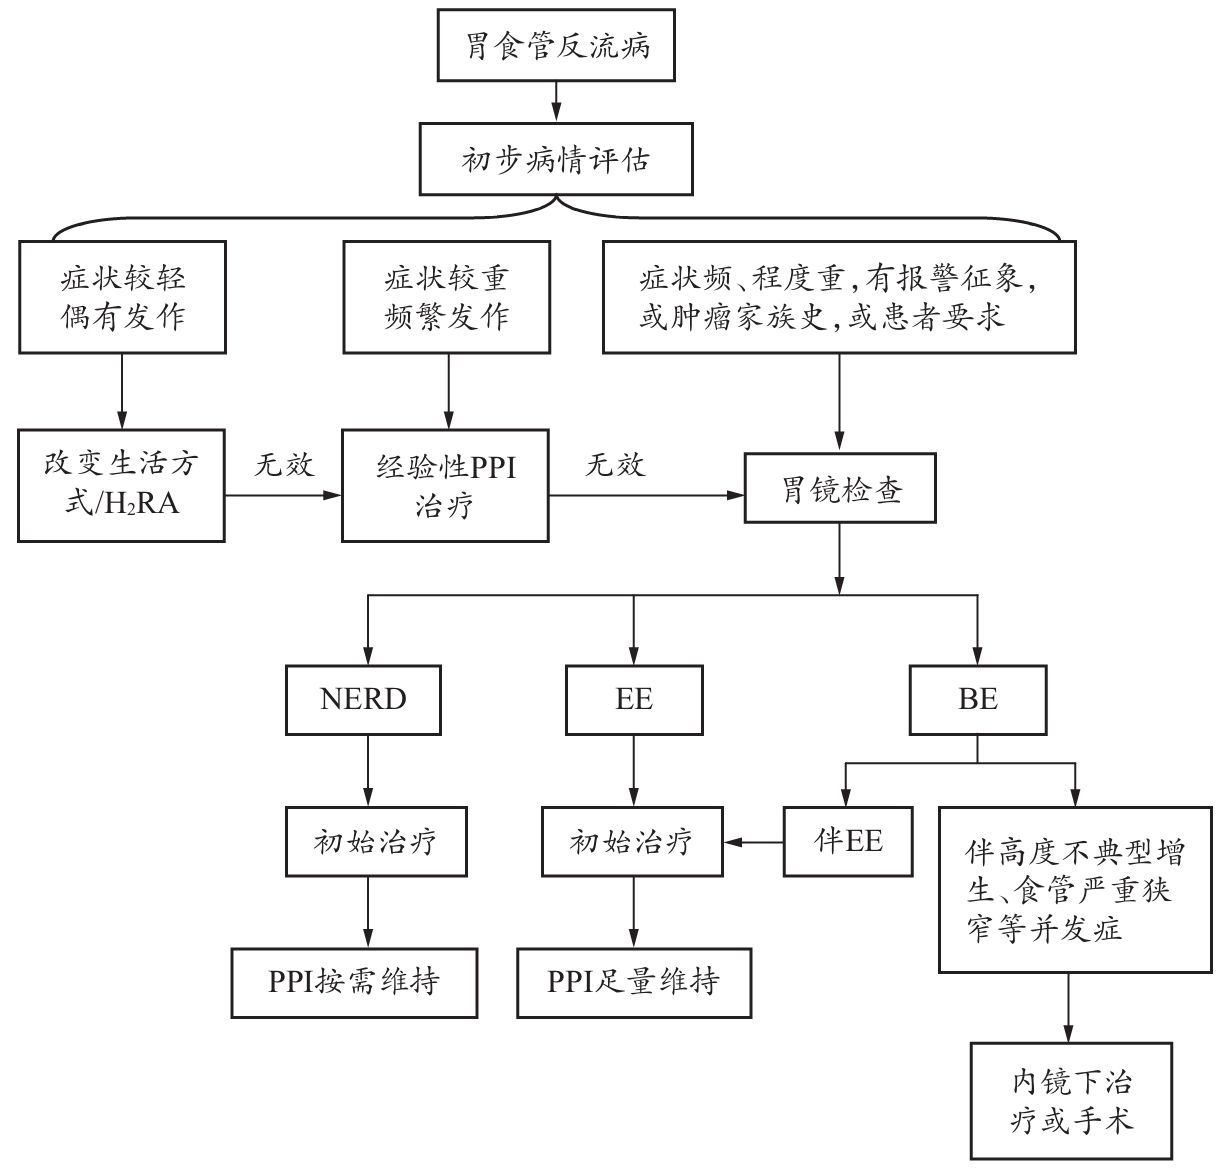
\includegraphics{./images/Image00085.jpg}
 \captionsetup{justification=centering}
 \caption{胃食管反流病的治疗程序}
 \label{fig3-1-1}
  \end{figure} 

【治疗方案】

1.
一般治疗 包括减肥、戒烟酒、低脂低糖饮食、避免饱食及减少摄入可以降低食管下段括约肌(LES)压力的食物(如巧克力、薄荷、咖啡、洋葱、大蒜等),睡前3小时不再进食、睡时抬高床头、白天进餐后亦不宜立即卧床等,但这些改变对多数患者并不足以缓解症状。目前尚无关于改变生活方式对GERD治疗的对照研究。

2.
药物治疗 包括抑制胃酸分泌药物和促动力药物。抑制胃酸分泌是目前治疗GERD的基本方法,包括H{2}
受体拮抗剂(H{2} RA)和质子泵抑制剂PPI等。H{2}
RA包括如西咪替丁、雷尼替丁、法莫替丁等,仅适用于轻至中度GERD的初始治疗和症状短期缓解,4\textasciitilde{}6周后大部分患者出现药物抵抗,长期疗效不佳。PPI包括如奥美拉唑、兰索拉唑、泮托拉唑、雷贝拉唑和埃索美拉唑等,抑酸能力强,是GERD治疗中最常用的药物。促动力药物可作为抑酸治疗的辅助用药,包括如多潘立酮、莫沙必利、依托必利等。在抑酸药物治疗效果不佳时,可考虑联合应用促动力药物,特别是对于伴有胃排空延迟的患者。

(1)拟诊GERD的治疗:根据MontrealGERD的新定义,对有典型反流症状的患者,如无出血、吞咽困难等报警症状,临床上便可拟诊为GERD,即可给予PPI经验性治疗:采用PPI标准剂量,每日2次,时间1\textasciitilde{}2周,如患者症状得到改善,则支持为与酸相关的GERD;否则可能有酸以外的因素或不支持诊断。对于疗效不佳患者建议行胃镜检查,明确诊断后再进行治疗。

(2)非糜烂性反流病(NERD)的治疗:NERD的发病机制复杂,使用PPI控制症状的疗效不如糜烂性食管炎,但PPI仍是治疗NERD的主要药物,初始治疗的疗程尚未明确,有研究资料显示不少于8周,之后实行按需维持治疗。对疗效不佳者应进一步寻找影响疗效的原因。

(3)糜烂性食管炎(EE)的治疗:采用PPI标准剂量,初始治疗疗程为8周,部分患者症状控制不满意时可加大剂量或换1种PPI。之后以PPI标准剂量维持治疗,半年后随访80\%以上患者仍可维持正常。

(4)Barrett食管(BE)的治疗:PPI能延缓BE的进程,但尚无足够的循证依据证实其能逆转BE。BE伴有糜烂性食管炎及反流症状者,使用大剂量PPI治疗,并提倡长期维持治疗。BE伴高度不典型增生、食管严重狭窄等并发症,可考虑内镜或手术治疗。

(5)控制夜间酸突破(NAB):NAB指在每天早、晚餐前服用PPI的情况下,夜间胃内pH\textless{}4持续时间大于1小时,控制NAB是治疗GERD的措施之一。治疗方法包括调整PPI用量、睡前加用H{2}
RA、应用血浆半衰期更长的PPI等。

【疗效观察与随访】

1.
观察指标 观察治疗前后患者的症状如反流、烧心、胸骨后疼痛以及食管外症状如咽炎等变化情况,以及胃镜下观察病变以及病理改善情况。

2.
治愈标准 症状消失,X线检查、内镜检查恢复正常。若症状减轻,上述检查基本恢复为临床好转。

3. 随访 注意病情观察,避免并发症,严防恶变。

【治疗经验与解析】

1.
对于拟诊为GERD的患者,如年龄大于40岁,发病后体重显著减轻,出现呕血、吞咽困难等症状时应首先行胃镜检查,明确诊断后再进行治疗。

2.
对PPI治疗失败的患者,应积极寻找原因,对症处理。其中可能的原因有:①患者依从性差,服药不正规;②与个体差异有关;③存在NAB;④内脏高敏感;⑤存在碱反流。

3.
对于产生食管狭窄并发症的患者,除极少数瘢痕狭窄严重需行手术切除外,绝大部分可行内镜下食管扩张术治疗。扩张术后予以长程PPI维持治疗可防止狭窄复发,对顽固性患者亦可考虑抗反流手术。

4.
Barrett食管恶变为食管腺癌的危险性高,加强随访尤其是内镜检查是目前预防Barrett食管癌变的唯一方法。重点在于早期识别异型增生,发现重度异型增生或早期食管癌,及时手术切除,根据情况可选择内镜下粘膜切除术(EMR)、粘膜剥离术(ESD)或者手术治疗。

5.
本病需进一步与药物性食管炎、霉菌性食管炎、腐蚀性食管炎、免疫相关的食管病变以及食管癌鉴别,了解患者既往病史及家族史,行胃镜及镜下病理检查有利于鉴别诊断。如以胸痛为主要临床表现者,应与心源性胸痛及其他原因引起的非心源性胸痛进行鉴别。

6.
改变生活方式与饮食习惯,包括减肥、戒烟酒、低脂低糖饮食、避免饱食;避免睡前2小时内进食,白天进餐后亦不宜立即卧床;卧位时可将床头抬高15\textasciitilde{}20cm;减少引起腹压增高的因素,如便秘、紧束腰带等;应避免进食使LES压降低的食物,如高脂肪、巧克力、咖啡、浓茶等;避免应用降低LES压的药物及引起胃排空延迟的药物。


\subsection{食管癌}

食管癌(carcinoma of the
esophagus)是原发于食管的恶性肿瘤。食管癌的病理类型分为鳞癌和腺癌,在全球食管癌高发区鳞癌最常见,如中国;但是在食管癌非高发区,腺癌却是最常见的病理类型,如北美洲和许多西欧国家。临床上食管癌以进行性吞咽困难为其典型症状。对于出现进食后胸骨后停滞感或咽下困难的患者,及时做有关检查,如内镜与组织活检病理检查、超声内镜、食管X线钡餐造影、CT扫描等,确诊一般无困难。

【治疗程序】 如图\ref{fig3-1-2}\footnote{ESD:内镜粘膜下剥离术;EMR:内镜粘膜切除术}所示。

\begin{figure}[!htbp]
 \centering
 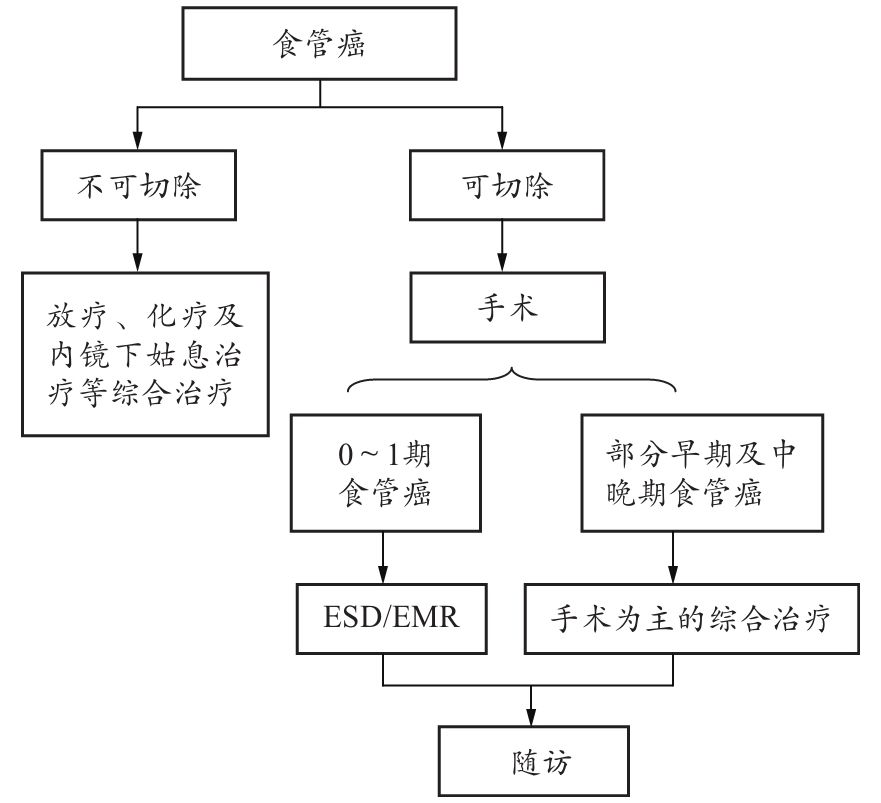
\includegraphics{./images/Image00086.jpg}
 \captionsetup{justification=centering}
 \caption{食管癌的治疗程序}
 \label{fig3-1-2}
  \end{figure} 

【治疗方案】 治疗关键在于早期发现、早期诊断,对病情进行充分评估,包括分期、分级等,选择合适的个体化治疗方案,以期最大限度的根治、控制肿瘤,改善患者生活质量和预后。治疗方法包括内镜下治疗、手术、放疗、化疗、分子靶向治疗、中医中药等综合治疗。

AJCC食管癌TNM分期见表\ref{tab3-1-1}:


\begin{table}[htbp]
    \centering
    \caption{AJCC食管癌TNM临床分期}
    \label{tab3-1-1}
    \begin{tabular}{llll}
\toprule
临床分期 & T & N & M\tabularnewline
\midrule
0 & Tis & N0 & M0\tabularnewline
Ⅰ & T1 & N0 & M0\tabularnewline
ⅡA & T2 & N0 & M0\tabularnewline
& T3 & N0 & M0\tabularnewline
ⅡB & T1 & N1 & M0\tabularnewline
& T2 & N1 & M0\tabularnewline
Ⅲ & T3 & N1 & M0\tabularnewline
& T4 & AnyN & M0\tabularnewline
Ⅳ & AnyT & AnyN & M1\tabularnewline
ⅣA & AnyT & AnyN & M1a\tabularnewline
ⅣB & AnyT & AnyN & M1b\tabularnewline
\bottomrule
    \end{tabular}
\end{table}

组织学分级(G):GX:分级不明 G1:高分化 G2:中分化 G3:低分化 G4:未分化

1.
内镜下切除术 包括内镜下粘膜切除术(EMR)和内镜粘膜下层剥离术(ESD)。对于消化道早期病变,EMR和ESD疗效确切,创伤小,避免患者手术的痛苦。早期食管癌为EMR或ESD的适应证,是指癌瘤局限于食管粘膜层及粘膜下组织,未侵及肌层,没有淋巴转移的表浅癌,相当于食管癌国际TNM分期系统的0期\textasciitilde{}1期。

2.
手术治疗 对可切除疾病来说,外科手术是标准处理方法。食管癌手术适应证为分期在T1\textasciitilde{}T4、N0\textasciitilde{}1、NX或者ⅣA一般情况良好的患者。根据患者的一般情况、病情、肿瘤大小和部位、合并症等选择适合的术式。手术治疗的目的是尽可能达到R0切除(显微镜下达到完全切除)。对于术前明确不能完全根治的患者或晚期患者,尽可能避免姑息切除,而采取非手术的综合治疗模式。术前辅助治疗结合手术与单纯手术相比,对生存期没有太大影响。

3.
放疗 单纯放疗只用于不能接受化疗的患者或作为姑息治疗。对于姑息治疗,主要针对手术难度大的上段食管癌和不能切除的中、下段食管癌。上段食管癌放疗效果不亚于手术,故放疗作为首选。在辅助治疗方面,临床研究没有明确证据能够说明术前或术后单纯放疗能够延长生存期。近年来有研究将放射粒子捆绑于食管支架制成内照射支架进行单纯近距离放疗,因操作技术复杂,难以保证手术成功率,且不能够避免对环境的污染,对操作者的辐射伤害,临床较少应用,疗效和安全性有待进一步观察。

4.
化疗 对于姑息治疗,放疗等其他手段包括联合方案相较于单纯化疗更有效。根据临床研究结果,不推荐术前化疗作为标准治疗手段。同样,术后化疗现在也没有比较标准的系统的方案。

与腺癌相比,鳞癌对化疗、放疗或放化疗更为敏感,然而两种病理类型在远期预后方面并没有太大区别。联合5-FU和DDP方案是研究与应用最多的方案,有效率在20\%\textasciitilde{}50\%之间。紫杉醇联合5-FU和DDP是对鳞癌和腺癌都有效的方案。另外,联合伊立替康和DDP有效,特别是对食管鳞癌。尽管联合化疗有很高的反应率,但并发症的发生率也较高。

5.
联合放、化疗 由于临床上食管癌术后复发转移率较高,有些术后分期早的患者同样存在复发转移的高风险,单纯手术切除的长期生存率较低,因此食管癌的辅助治疗仍是人们关注的焦点,目前往往采用联合放化疗的综合治疗。两者可同时进行也可序贯应用,化疗可加强放疗的作用,但严重不良反应发生率较高。

但是随机临床试验结果中,术前联合放化疗和单纯手术相比的优劣仍存在争议,一项荟萃分析表明,术前联合放化疗与单纯手术相比,明显提高3年生存率、降低局部复发率和使肿瘤降期,但术后死亡率明显升高;另一项研究结果表明两组的生存率相似。因此,术前联合放化疗虽然合理,但仍需继续研究。

6.
分子靶向治疗 2009年NCCN指南开始将曲妥珠单抗联合化疗作为人表皮生长因子受体(HER-2)阳性晚期食管癌的标准治疗之一。其余的分子靶向药物有西妥昔单抗、吉非替尼、厄洛替尼、贝伐单抗等,其疗效有待后续的临床研究进一步明确。但这些靶向药物尚缺少应用于食管鳞癌的研究数据,而我国食管癌以鳞癌为主,亟待开展相关研究,从而推进食管鳞癌的分子靶向药物治疗。

7.
食管癌性狭窄的内镜下姑息治疗 对于失去外科手术机会或是术后复发的中晚期食管癌患者,在不能耐受或不愿选择放、化疗或是放疗后出现严重并发症的情况下,为解决进食梗阻,需行内镜下姑息治疗,方法包括:

(1)单纯扩张:方法简单,但作用时间短且需反复扩张;对病变范围广泛者常无法应用。

(2)食管内支架置入术:是在内镜直视下放置合金或塑胶的支架,可达到较长时间缓解梗阻或封堵食管气管瘘,提高生活质量,但上端食管癌与食管胃连接部肿瘤支架放置较困难。

(3)内镜下实施癌肿消融术。

【疗效观察与随访】

1.
观察指标 治疗前后患者的症状如进食梗阻等变化情况;实验室检查项目如血常规、血生化、肿瘤指标等;内镜和其他影像学如胸片、胸部CT、PET等器械检查项目。

2. 治愈标准 术后肿块消失,肿瘤标志物转阴,全身状况良好。

3.
随访 所有患者都应系统地随访。随访应该包括:第1年每4个月进行一次完整的病史询问和体格检查,随后每6个月一次,持续两年,其后每年1次。根据临床指征决定进行血常规、血生化、肿瘤指标和胸片检查等。如有临床症状如持续性或反复吞咽困难等应相应进行内镜和其他影像学检查。另外,对于由于吻合口或放化疗引起的狭窄,有些患者需要进一步行扩张治疗。

【治疗经验与解析】

1.
无论采用EMR或ESD,治疗前均应进行食管超声内镜及高频超声微探头技术准确评估病灶的浸润深度并排除淋巴结转移,应用染色内镜技术确定病灶范围;切取标本应整块送检,进一步明确病灶切除是否彻底及病灶的浸润深度,评估术后是否需补救治疗;术后应有良好的随访条件及严格的随访制度。

2.
目前通常采用的治疗方法是:对于可切除的食管癌,术前化放疗加手术是最合适的方法。对晚期不可切除的食管癌,化放疗最合适,在某些病例,也许能变为可切除食管癌。对可切除但不采取手术的患者,根治性化放疗是合适的选择。对于不能手术且不能耐受放化疗的患者,可行内镜下姑息治疗,解决进食梗阻,提高生活质量。

3.
对于Barrett食管,需应用组胺受体拮抗剂或质子泵抑制剂控制胃食管反流症状,并行内镜检查随访,评估化生、轻度不典型增生(LGD)、重度不典型增生(HGD)或腺癌。如为食管粘膜化生,应每1\textasciitilde{}3年例行内镜检查外加4象限活检;如果是LGD,检查间期降为6\textasciitilde{}12个月;如果在随访中发现HGD,需经第二位病理学家进一步病理确诊。实际上相当比例的HGD患者在诊断时就已经为隐性腺癌,这部分患者应采取手术切除,以后进行终身随访---------每3个月一次内镜检查及深部活检。

4.
本病需与一些食管的良性病变如食管贲门失弛缓症、胃食管反流病、食管良性狭窄以及食管的良性肿瘤如食管平滑肌瘤等相鉴别。另外,对于有进食梗阻感的患者,还需与食管裂孔疝、食管静脉曲张、纵隔肿瘤、食管周围淋巴结肿大、左心房明显增大、主动脉瘤外压食管造成狭窄以及无器质性病变的癔球症等相鉴别。

5.
避免高危因素如吸烟、大量饮酒及进食过烫等,改变不良的生活习惯如避免进食霉变和含亚硝铵成分高的食物,改良饮水,防霉去毒,改善营养卫生等。在食管癌高发区建立了防治基地,对高危人群进行普查和筛查以期早期发现食管癌,必要时行化学药物干预治疗。


\section{胃炎}

胃炎(gastritis)是指任何病因引起的胃粘膜炎症,常伴有上皮损伤和细胞再生。胃炎是最常见的消化道疾病之一。按临床发病的缓急和病程的长短,一般将胃炎分为急性胃炎和慢性胃炎。

\subsection{急性胃炎}

急性胃炎指由不同原因所致胃粘膜的急性炎症和损伤。常见病因有酒精、药物、应激、感染、十二指肠反流液、胃粘膜缺血、缺氧、变质食物和不良饮食习惯、腐蚀性物质以及放射损伤或机械损伤等。急性胃炎以急性上腹痛、饱胀、恶心、呕吐、嗳气和食欲减退等为常见的主要临床症状,重症者还可出现呕血或黑便等上消化道出血症状,甚至以此为首发表现,出血量大时可导致失血性休克。内镜检查可见胃粘膜充血、水肿、出血、糜烂(可伴有浅表溃疡)等一过性病变。

【治疗程序】 如图\ref{fig3-2-1}所示。

\begin{figure}[!htbp]
 \centering
 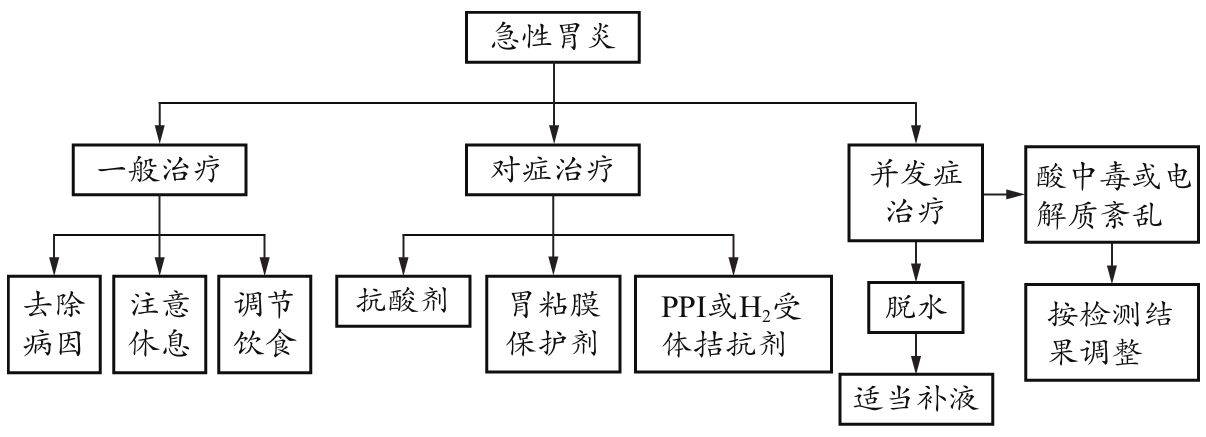
\includegraphics{./images/Image00087.jpg}
 \captionsetup{justification=centering}
 \caption{急性胃炎的治疗程序}
 \label{fig3-2-1}
  \end{figure} 

【治疗方案】

1.
一般治疗 去除病因,积极治疗原发病,并针对原发病和病因采取防治措施,保证休息,进清淡饮食,必要时可短期禁食。

2.
药物治疗 (1)抑制胃酸分泌:急性胃炎的主要治疗药物为抑制胃酸分泌制剂,包括质子泵抑制剂PPI和H{2}
受体拮抗剂(H{2} RA)等。

(2)胃粘膜保护剂和抗酸剂:硫糖铝、胶体铋、氢氧化铝凝胶剂或其与氢氧化镁的混合剂,每日3\textasciitilde{}4次口服。

(3)细菌感染性急性胃炎:可进一步加用适当的抗感染药物,如氟喹诺酮类制剂、氨基糖苷类制剂或头孢菌素。如左氧氟沙星0.2g口服,每日2次。

(4)急性糜烂出血性胃炎发生上消化道大出血者:按上消化道出血治疗原则采取综合措施进行治疗,PPI和H{2}
RA静脉给药可促进病变愈合和有助止血,为常规应用药物。临床常用奥美拉唑40\textasciitilde{}80mg静脉注射或静脉滴注,每日2\textasciitilde{}3次。

(5)对症支持治疗:恶心、呕吐明显者,可使用甲氧氯普胺(胃复安)、多潘立酮(吗丁啉)等胃动力药物。呕吐患者不能进食,应注意补液,维持水、电解质、酸碱平衡。腹痛者可选用阿托品、复方颠茄片或山莨菪碱等解痉药。

【疗效观察与随访】

1.
观察指标 观察治疗前后患者的症状变化情况,如急性上腹痛、饱胀、恶心、呕吐、嗳气、呕血、黑便等,以及胃镜下观察镜下病变改善情况。细菌感染者还需观察血常规变化情况。

2. 治愈标准 症状、体征消失,1个月内无复发。

3. 随访 注意病情观察,避免并发症。

【治疗经验与解析】

1.
按照病理生理的不同,通常将急性胃炎分为急性单纯性胃炎、急性糜烂出血性胃炎、特殊病理引起的急性胃炎如急性腐蚀性胃炎、急性化脓性胃炎等。临床上以急性单纯性胃炎最为常见,通常由不洁饮食引起,常合并急性肠炎。另外,非甾体类消炎药和应激引起的急性糜烂出血性胃炎临床上亦较为常见,又称为急性胃粘膜病变,其临床表现可无症状或被基础疾病所掩盖,常在发生消化道出血时才引起重视。急性胃粘膜病变也是急性上消化道出血的常见病因之一。

2.
有近期服用NSAID史、严重疾病状态、大量饮酒或精神应激的患者,如发生呕血和(或)黑便,应考虑急性糜烂出血性胃炎的可能,条件许可应行急诊胃镜检查。内镜下可见以弥漫分布的多发性糜烂、出血灶和浅表溃疡为特征的急性胃粘膜病损。

3.
本病需与急性阑尾炎早期、急性胆囊炎、急性胰腺炎、肾绞痛等相鉴别,密切观察病情变化。

4.
在日常生活中应注意饮食卫生,不食用不洁食物或酗酒,不暴饮暴食,不服刺激性食物和乱服药物,必须服用阿司匹林及其他NSAID制剂患者,应视情况使用PPI预防。避免过度疲劳;增强体质,坚持规律、适度的运动。另外,对于可产生内源性刺激因素的原发病给予足够的重视,去除病因。


\subsection{慢性胃炎}

慢性胃炎是指胃粘膜慢性炎症或萎缩。慢性胃炎分为非萎缩性(浅表性)胃炎和萎缩性胃炎两大基本类型,同时存在平坦糜烂、隆起糜烂、出血、粗大皱襞或胆汁反流征象,则诊断为非萎缩性(浅表性)或萎缩性胃炎伴糜烂、胆汁反流等。根据病变分布可分为胃窦炎、胃体炎、全胃炎胃窦为主或全胃炎胃体为主。多数慢性胃炎患者无临床症状,有症状者主要表现为上腹痛或不适、上腹胀、早饱、嗳气、恶心等非特异性消化不良;有无消化不良症状及慢性胃炎的严重程度与内镜所见和组织学分级无相关性。胃体萎缩性胃炎合并恶性贫血者可出现贫血貌、全身衰竭、乏力、精神淡漠,而消化道症状可以不明显。慢性胃炎的确诊主要依赖内镜检查和胃粘膜活检组织学检查。幽门螺杆菌(Hp)感染是慢性胃炎的主要病因,检测幽门螺杆菌有助于病因诊断及治疗、预防复发。

【治疗程序】 如图\ref{fig3-2-2}所示。

\begin{figure}[!htbp]
 \centering
 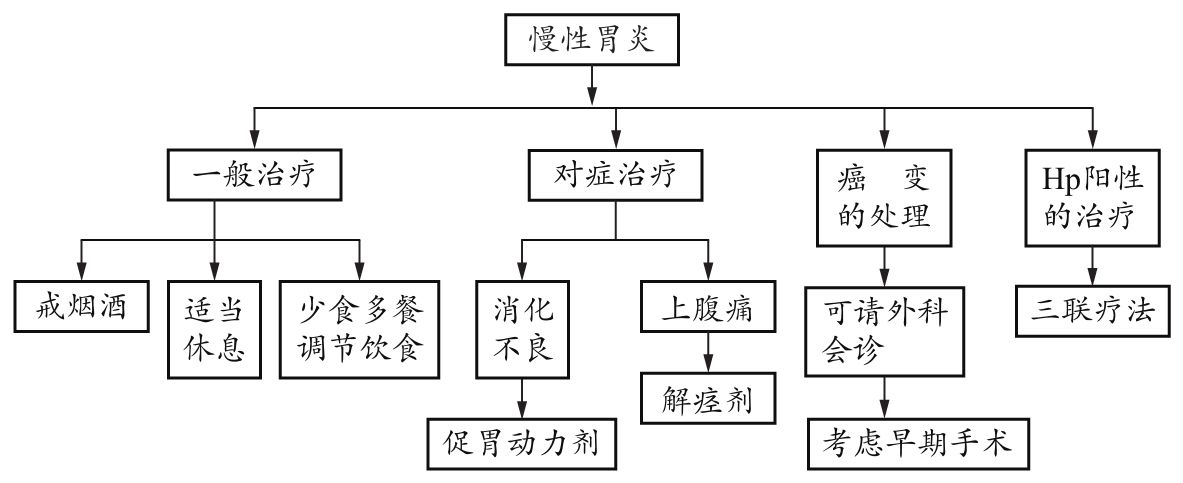
\includegraphics{./images/Image00088.jpg}
 \captionsetup{justification=centering}
 \caption{慢性胃炎的治疗程序}
 \label{fig3-2-2}
  \end{figure} 

【治疗方案】 治疗目的是缓解症状和改善胃粘膜组织学。治疗应尽可能针对病因,遵循个体化原则。

1.
一般治疗 积极治疗口鼻咽部感染,戒烟戒酒。饮食宜软、易消化且规律,避免暴饮暴食,忌含浓烈辛辣调料的食品或服用对胃有刺激的药物,生活规律,保持心情愉悦和心态平和。

2. 药物治疗

(1)对症治疗:慢性胃炎伴有消化不良症状的患者的主要治疗内容为改善症状。有胃粘膜糜烂和(或)以反酸、上腹痛等症状者可选用抑酸或抗酸药如PPI;症状明显者可加用胃粘膜保护剂;以上腹饱胀、恶心或呕吐等为主要症状者可应用促动力药;伴胆汁反流者则可应用促动力药和(或)有结合胆酸作用的胃粘膜保护剂;上腹饱胀、纳差等症状明显者可补充消化酶制剂如多酶片或胰酶片,并且对慢性萎缩性胃炎无粘膜糜烂尤其是胃体萎缩性胃炎者适用。具体药物见本书胃食管反流病和急性胃炎章节。

(2)根除幽门螺杆菌治疗:对于幽门螺杆菌引起的慢性胃炎是否应常规根除幽门螺杆菌尚缺乏统一意见。但根除Hp可消除或改善胃粘膜炎症,防止萎缩、肠化进一步发展,预防消化性溃疡及降低胃癌发生的危险性,部分患者消化不良症状也可取得改善,参见表\ref{tab3-2-1}。

\begin{table}[htbp]
    \centering
    \caption{根除幽门螺杆菌常用的治疗方案}
    \label{tab3-2-1}
    \begin{tabular}{lp{6cm}l}
\toprule
方案 & 药物(选用常规剂量) & 疗程(日)\tabularnewline
\midrule
一线方案:三联疗法 &
\vtop{\hbox{\strut PPI+克拉霉素+阿莫西林}\hbox{\strut 或PPI+克拉霉素+甲硝唑(或替硝唑)}}
& 7\textasciitilde{}14\tabularnewline
二线方案:四联疗法 &
PPI+铋剂+2种抗生素(克拉霉素、阿莫西林、甲硝唑、替硝唑、呋喃唑酮、左氧氟沙星)
& 10\textasciitilde{}14\tabularnewline
序贯疗法 &
前5日为PPI+阿莫西林,后5日为PPI+克拉霉素+替硝唑;或前5日为PPI+克拉霉素,后5日为PPI+阿莫西林+呋喃唑酮
& 10\textasciitilde{}14\tabularnewline
\bottomrule
    \end{tabular}
\end{table}

根据2006年中国慢性胃炎共识意见,根除幽门螺杆菌特别适用于:

1)伴有胃粘膜糜烂、萎缩及肠化生、异型增生者。

2)有消化不良症状者。

3)有胃癌家族史者。

目前推荐的各类根除Hp治疗方案中最常用的是以PPI为基础的三联治疗方案(PPI、阿莫西林、克拉霉素),三种药物均采用常规剂量,疗程7\textasciitilde{}14日。对于首次根除失败者,应采用二、三线方案进行治疗。二、三线方案常用四联疗法,可根据既往用药情况并联合药敏试验,采取补救治疗措施(PPI+铋剂+2种抗生素)或选用喹诺酮类、呋喃唑酮、四环素等药物,疗程多采用10日或14日。或采用序贯疗法,根除Hp具有疗效高、耐受性和依从性好等优点。序贯疗法为10日:前5日为PPI+阿莫西林,后5日为PPI+克拉霉素+替硝唑;或前5日为PPI+克拉霉素,后5日为PPI+阿莫西林+呋喃唑酮。据报道序贯疗法有效率达90\%以上。但对序贯疗法国内仍需积累更多的临床经验。

(3)自身免疫性胃炎的治疗:目前尚无特异治疗,合并恶性贫血者需终身补充维生素B{12}
。有缺铁性贫血者补充铁剂,同时加用维生素C,有利铁剂吸收。可适当补充一些微量元素如锌、硒、β胡萝卜素等。

(4)内镜或手术治疗:萎缩性胃炎和肠化不是内镜或手术的绝对指征,对伴有息肉、异型增生或有局灶性凹陷或隆起者,应加强随访。对肯定的重度异型增生则宜予预防性手术,目前多采用内镜下胃粘膜切除术(EMR)。当慢性萎缩性胃炎伴重症异型增生或重度肠化生,尤其是大肠型肠化者可考虑手术治疗。

【疗效观察与随访】

1. 观察指标

(1)症状、体征:观察上腹痛或不适、上腹胀、早饱、嗳气、恶心、呕吐、纳差等消化不良症状的改善情况。上腹部压痛、舌苔等改善情况。

(2)血常规:对伴有贫血的胃体胃炎应监测血常规情况。

(3)定期复查Hp。

2.
治愈标准 症状、体征消失,相关检查正常,半年内无复发。若症状、体征基本消失,相关检查基本正常,为好转。

3.
随访 注意病情变化,跟踪监测胃镜及组织病理学情况,避免并发症尤其是胃癌的发生。

【治疗经验与解析】

1. 无症状、Hp阴性的非萎缩性胃炎无须特殊治疗。

2.
有明显精神因素的慢性胃炎伴消化不良症状患者,需耐心解释或心理治疗,必要时可使用抗抑郁药或抗焦虑药物。

3. 中药治疗可拓宽慢性胃炎的治疗途径。

4.
需与本病相鉴别的疾病有胃食管反流病、消化性溃疡、胃癌等上消化道疾病,行胃镜及镜下病理检查有利于鉴别诊断。以腹痛为主要表现者,需与慢性胆囊炎、慢性胰腺炎、肝病等肝、胆、胰疾病相鉴别,腹部B超检查有助于鉴别。

5.
饮食、生活规律,避免暴饮暴食和辛辣刺激饮食,戒烟戒酒,保持心情愉悦和心态平和。避免受凉、劳累,参加适当的体育锻炼,增强体质。

\section{消化性溃疡}

消化性溃疡病是常见的消化系疾病,指在各种致病因子的作用下,消化道粘膜发生的炎症与坏死性病变,病变深达粘膜肌层,常发生于胃酸分泌有关的粘膜,以胃、十二指肠为最常见。消化性溃疡病的发病机制,主要与胃、十二指肠粘膜的损害因子和粘膜自身防御修复因子之间失衡有关,常见有胃酸分泌异常、Hp感染、NSAID和糖皮质激素药物等。近年来,由于抗酸剂、抑酸剂等广泛使用,非典型的患者日益增多,部分以上消化道出血为首发症状。随着胃镜检查的普及,胃镜联合病理检查诊断消化性溃疡并不困难。对于消化性溃疡病患者还需同时行Hp感染情况的检测。

【治疗方案】 主要分为四个方面,即一般治疗、药物治疗、并发症治疗和外科手术及内镜下治疗。治疗目的主要是缓解症状、促进溃疡愈合、防治并发症和预防复发。

1.
一般治疗 消除病因,禁用或慎用对胃粘膜有损伤的药物。注意饮食卫生,戒烟戒酒,生活规律,保持心情愉悦和心态平和。

2. 药物治疗

(1)抑制胃酸分泌:是缓解消化性溃疡病症状、愈合溃疡的最主要措施,包括PPI和H{2}
RA,其中PPI是首选药物,通常采用标准剂量的PPI,每日1次,早餐前半小时服药。治疗十二指肠溃疡疗程为4周,胃溃疡为6\textasciitilde{}8周。

(2)胃粘膜保护剂和中和胃酸药物:联合应用粘膜保护剂可提高消化性溃疡病的愈合质量,有助于减少溃疡的复发率。中和胃酸药有助于缓解消化性溃疡病腹痛、反酸等症状,促进溃疡愈合。胃粘膜保护剂和中和胃酸药物有替普瑞酮、胶体铋、麦滋林-S颗粒、吉法酯、硫糖铝、氢氧化铝凝胶剂或其与氢氧化镁的混合剂等,每日3\textasciitilde{}4次口服。

(3)对症支持治疗:腹胀、恶心、呕吐明显者,可使用甲氧氯普胺(胃复安)、多潘立酮(吗丁啉)、莫沙比利等胃动力药物。腹痛者可用阿托品、复方颠茄片或山莨菪碱等解痉药。

(4)抗幽门螺杆菌治疗:根除Hp以作为消化性溃疡病的基本治疗,它是溃疡愈合及预防复发的有效防治措施。对Hp检测阳性者均应行抗Hp治疗。具体治疗方案见本书慢性胃炎章节。

(5)消化性溃疡病合并活动性出血:首选治疗方法是内镜下止血,同时使用PPI可有效预防再出血,减少外科手术率与死亡率。

3.
内镜下治疗 如上所述,消化性溃疡病合并活动性出血首选内镜下止血。消化性溃疡致瘢痕性幽门梗阻者可通过内镜下扩张治疗缓解病情,减轻进食梗阻,改善生活质量。

4.
外科手术 外科手术的指证包括:①大量出血经内科治疗无效;②急性穿孔;③瘢痕性幽门梗阻;④胃溃疡癌变;⑤严格内科治疗最终无效的顽固性溃疡。目前由于内科治疗的进展,消化性溃疡病并发症的发生率已大大降低,仅少数并发症患者需要外科手术治疗。

【疗效观察与随访】

1. 观察指标

(1)症状、体征:观察上腹痛或不适、上腹胀、早饱、嗳气、恶心、呕吐、纳差等症状的改善情况。上腹部压痛等改善情况。

(2)胃镜及组织病理学改善情况。

(3)Hp感染转阴情况:治疗后应复查幽门螺杆菌是否已被根除,复查时间为根除幽门螺杆菌治疗结束至少4周,且在检查前停用PPI或铋剂2周,否则会出现假阴性。可采用非侵入性的{13}
C或{14}
C尿素呼气试验,也可通过胃镜在检查溃疡是否愈合的同时取活检做尿素酶及(或)组织学检查。

2.
治愈标准 症状、体征消失3个月以上,半年内无复发,各科相关检查均恢复正常。若症状、体征减轻,Hp转阴、GI龛影缩小,内镜下溃疡面缩小,粘膜充血水肿减轻为好转。

3. 随访 注意病情观察,避免并发症。必要时定期复查GI或胃镜、Hp等。

【治疗经验与解析】

1.
对老年人消化性溃疡病、巨大溃疡、复发性溃疡建议在抗酸、抗Hp治疗同时,应用胃粘膜保护剂。

2.
长期服用NSAID是导致消化性溃疡病复发的另一重要因素,如因原发的病情需要不能停药者,可更换环氧合酶抑制剂(COX-2),并同时服用PPI。但对有心脏病危险者不建议使用COX-2抑制剂。

3.
经正规系统治疗后仍未愈合的难治性消化性溃疡,Hp感染是一个重要因素。另外,可能的其他因素有:①穿透性溃疡;②特殊原因所致消化性溃疡,如胃泌素瘤;③某些伴随疾病或药物影响药物吸收或使效价减低;④误诊,如胃或十二指肠恶性肿瘤;⑤不良诱因存在,包括吸烟、酗酒、激素或NSAIDs的应用及精神应激等。

对于合并Hp感染的顽固性溃疡治疗,美国国立卫生研究院(NIH)推荐用奥美拉唑与抗生素联合治疗。其中,奥美拉唑20mg,口服,每日2次为宜。对于Hp阴性的顽固性溃疡,应去除诱因、系统治疗,使用强抗酸分泌药物如奥美拉唑或兰索拉唑等,并增加药量,延长用药时间。

4.
特殊类型的溃疡包括复合性溃疡、幽门管溃疡、球后溃疡、老年性溃疡及胃泌素瘤所致消化性溃疡。特殊类型的溃疡不具备典型溃疡的疼痛特点,往往缺乏疼痛的节律性。胃泌素瘤患者多有顽固性症状和多发性难治性溃疡。消化性溃疡病的主要并发症为上消化道出血、穿孔和幽门梗阻,胃溃疡还可能发生癌变。

5.
本病需与其他上消化道疾病如胃食管反流病、急慢性胃炎、胃癌、胃泌素瘤、功能性消化不良等相鉴别诊断,行胃镜及镜下病理检查有利于鉴别诊断,不能耐受胃镜检查者,X线钡餐检查发现龛影亦有确诊价值。以腹痛为主要表现者,需与胆囊炎、胰腺炎、肝病等疾病相鉴别,腹部B超、CT等检查有助于鉴别。另外,消化性溃疡病须与克罗恩病、结核、淋巴瘤、巨细胞病毒等继发性上消化道的溃疡相鉴别。

6.
注意生活与休息,调节精神情绪,戒烟戒酒,合理安排膳食,避免不规律饮食、暴饮暴食、冷硬粗糙食物、辛辣刺激食物,禁用或慎用对胃粘膜有损伤的药物。对于幽门螺杆菌复查阳性的患者,积极的再次根除幽门螺杆菌能大大减少溃疡复发。对于NSAID相关性溃疡,在基础疾病条件许可的情况下停服NSAID药物,可预防溃疡的复发。如基础疾病不允许停用NSAID药物的患者,以及曾有严重并发症的患者,可使用PPI长程维持治疗预防溃疡复发,剂量可为PPI常规剂量的半量。

\section{胃癌}

胃癌(gastric
carcinoma)约占胃恶性肿瘤的95\%以上。每年新诊断的癌症病例数中,胃癌位居第四位,在癌症病死率中列第二位。该病在我国仍是最常见的恶性肿瘤之一,死亡率下降并不明显。早期胃癌多无症状,进展期胃癌可出现的症状有上腹痛,常伴有纳差、厌食、体重减轻等;内镜检查结合粘膜活检,是目前诊断的金标准。外科手术切除加区域淋巴结清扫是目前根治胃癌的手段,早期胃癌可在内镜下行电凝切除或剥离切除术,胃癌对化疗不敏感。预后直接与诊断的分期有关,5年生存率较低(7\%\textasciitilde{}34\%)。

【治疗程序】 如图\ref{fig3-4-1}所示。

\begin{figure}[!htbp]
 \centering
 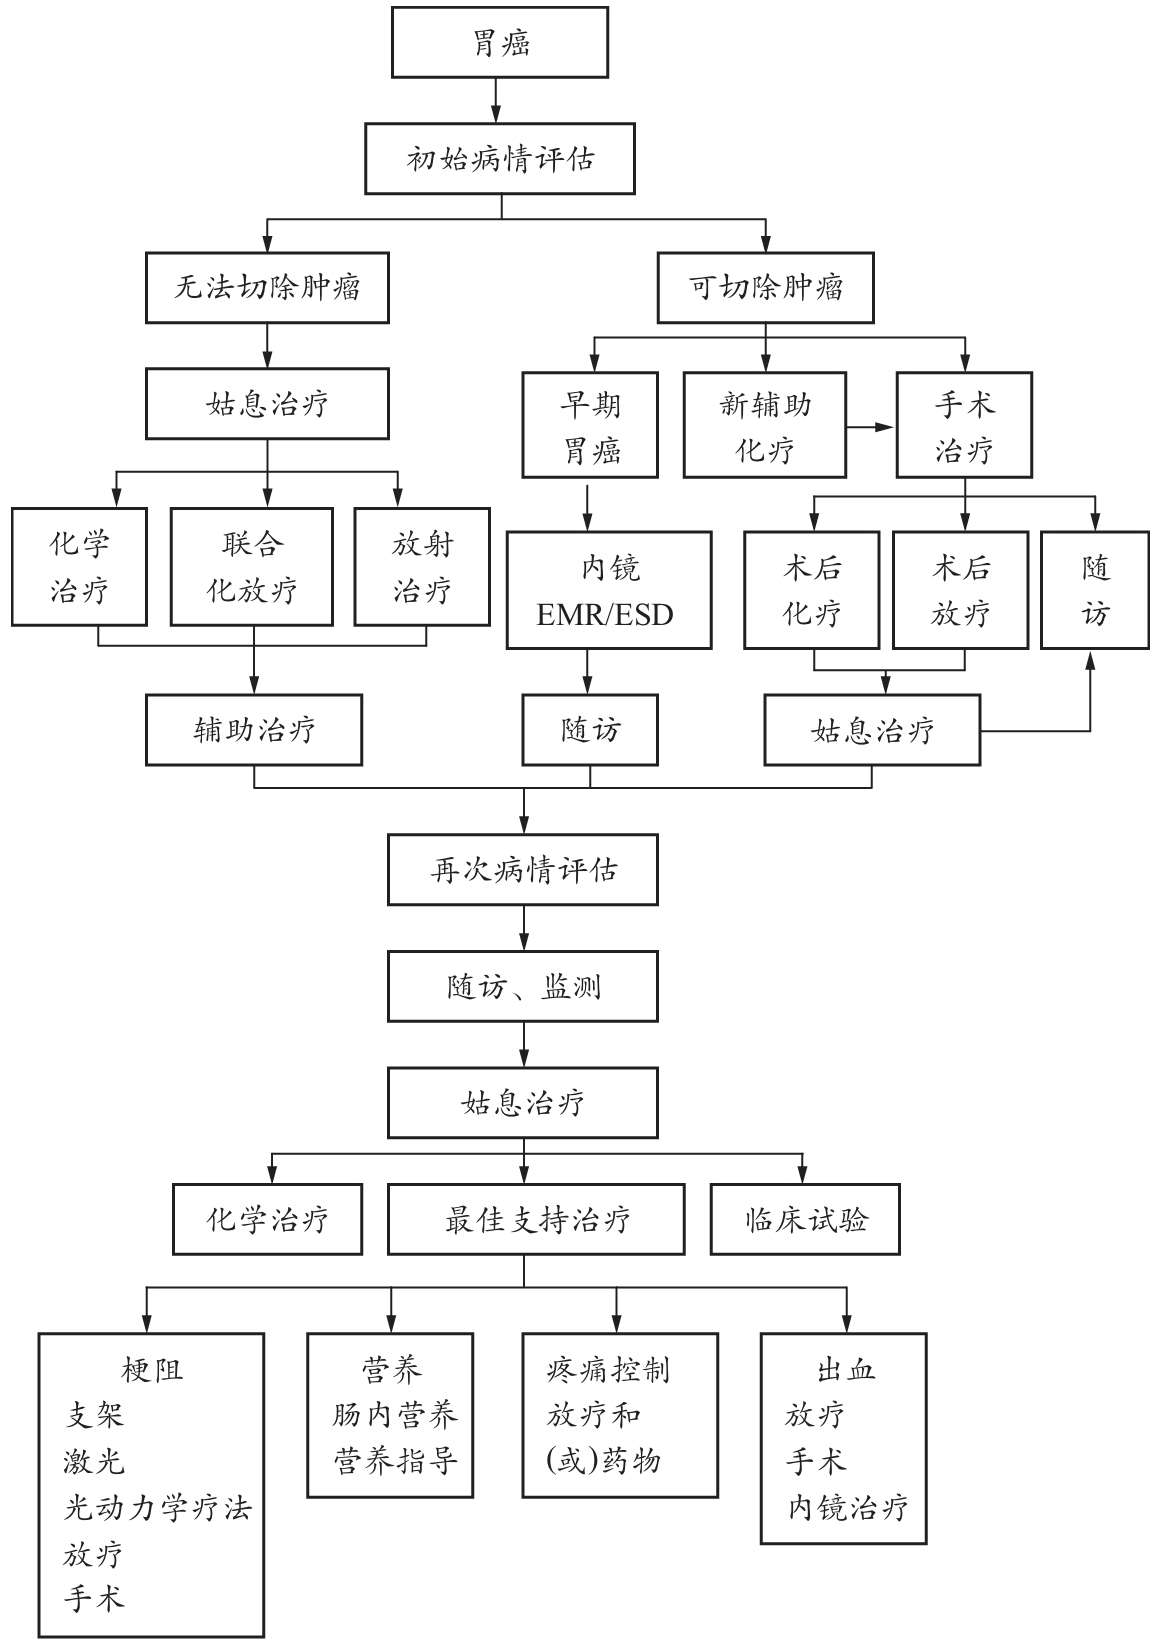
\includegraphics{./images/Image00089.jpg}
 \captionsetup{justification=centering}
 \caption{胃癌的治疗程序}
 \label{fig3-4-1}
  \end{figure} 

【治疗方案】

1.
手术治疗 外科手术切除加区域淋巴结清扫是目前治疗胃癌的手段。胃切除范围可分为近端胃切除、远端胃切除及全胃切除,近端切缘和远端切缘应距离肿瘤≥5cm,切除后分别用Billroth
Ⅰ、Billroth
Ⅱ及Roux-en-Y式重建消化道连续性,建议至少切除15个淋巴结并进行检查。手术效果取决于胃癌的分期、浸润的深度和扩散范围。对无法通过手术治愈的患者,部分切除仍然是缓解症状最有效的手段,特别是有梗阻的患者,术后有50\%的人症状能缓解,因此进展期胃癌,如果无手术禁忌证或远处转移,也应尽可能手术切除。

2.
内镜下治疗 早期胃癌可在内镜下行电凝切除或剥离切除术(EMR或ESD)。EMR适应证为肿瘤分化良好或中度分化、肿瘤直径小于30mm、无溃疡或肿瘤浸润的证据。由于早期胃癌可能有淋巴结转移,故需对切除的癌变病灶进行病理检查,如癌变累及到根部或表浅型癌肿侵袭到粘膜下层,需追加手术治疗。

3.
化学治疗 早期胃癌且不伴有任何转移灶者,手术后一般不需要化疗。胃癌对化疗并不敏感,目前应用的多种药物以及多种给药方案的总体疗效评价很不理想,尚无标准方案。化疗分为术前、术中、术后化疗:

(1)术前化疗即新辅助化疗:可使肿瘤缩小,增加手术根治及治愈机会。但有耐药克罗恩较早出现、可能会增加术后并发症的发生率且不易处理、使得术后病理分期不够精确、一部分患者可能会接受过度治疗、治疗前无法区分对治疗不敏感的患者而延误最佳手术时机等的问题。术前需要对肿瘤进行分期,制定合理的、个体化的治疗方案。

(2)术后辅助化疗:化疗对于进展期胃癌的中位生存时间仍然小于9个月。术后化疗方式主要包括静脉化疗、腹腔内化疗、持续性腹腔温热灌注和淋巴靶向化疗等。单一药物化疗只适合于早期需要化疗的患者或不能承受联合化疗者。常用药物有5-氟尿嘧啶(5-FU)、替加氟(FT-207)、卡培他滨、丝裂霉素(MMC)、阿霉素(ADM)或表阿霉素(EPB)、顺铂(DDP)或卡铂、亚硝脲类(CCNU,MeCCNU)、足叶乙甙(VP-16)等。联合化疗指采用两种以上化学药物的方案,一般只采用2\textasciitilde{}3种联合,以免增加药物毒副作用。

4.
放射治疗 胃癌对放射敏感性低,放疗在胃癌治疗中的作用主要是辅助性的或姑息性的。放疗的主要形式有术前放疗、术中放疗、术后放疗和姑息性放疗等四种。据文献报道术前放疗可使根治手术切除率提高2\%左右,使中晚期胃癌5年生存率提高1\%\textasciitilde{}2.5\%。

5.
中医中药治疗 中医认为胃癌多属于“反胃”、“胃脘痛”的范畴,病机是由于饮食不节,忧思过度,脾胃损伤,运化失司,痰湿内生,气结痰凝久则成积。

6.
其他 有实验表明生长抑素类似物及COX-2抑制剂能抑制胃癌生长,但其对人类胃癌的治疗尚需进一步的临床研究。

【疗效观察与随访】

1. 观察指标 观察治疗后患者症状、体征的变化:

(1)症状:胃癌最早出现的症状是上腹痛,常同时伴有纳差、厌食、体重减轻。腹痛开始仅为上腹饱胀不适,餐后更甚,偶呈节律性溃疡样疼痛,但这种疼痛不能被进食或服用制酸剂缓解。患者常有早饱感及软弱无力。

(2)体征:早期胃癌无明显体征,进展期在上腹部可扪及肿块,有压痛。如肿瘤转移至肝脏可致肝脏肿大及出现黄疸。腹膜有转移时可出现腹水至移动性浊音阳性。有远处淋巴结转移时可扪及质硬而不活动的Virchow淋巴结。

(3)副癌综合征:在一些胃癌患者可以出现,表现为反复发作的表浅性血栓静脉炎(Trousseau征)及过度色素沉着;黑棘皮症,皮肤褶皱处有过度色素沉着,尤其是双腋下;皮肌炎、膜性肾病、累及感觉和运动通路的神经肌肉病变等。

(4)观察有无并发症:如上消化道出血、幽门梗阻、穿孔、黄疸等。

(5)内镜检查:可直接观察胃内各部位,对胃癌,尤其对早期胃癌的诊断价值很大。

(6)X线钡餐检查:应用气钡双重对比法、压迫法和低张造影技术,采用高密度钡粉,能清楚地显示粘膜结构。癌的X线表现是胃壁僵硬失去蠕动。胃窦癌表现为胃窦狭窄,呈管状或漏斗状。弥漫性胃癌时受累范围广,胃容积变小,蠕动消失,呈革袋状。

(7)观察实验室检查指标:如大便隐血试验、肿瘤标志物及血细胞分析等。

2. 治愈标准 根治性手术切除后切口愈合,无并发症,5年无复发。

3.
随访 所有的胃癌患者都应该接受系统性的随访。随访的内容包括全面的病史询问和体格检查,全血细胞、血CEA、肝肾功能、胸部X线、腹部B超或CT、PET、内窥镜检查等。前3年每4\textasciitilde{}6个月一次,之后每年一次。对胃次全切除或全胃切除者每次随访应监测维生素B{12}
。

【治疗经验与解析】

1.
全世界胃癌治疗的最佳临床证据表明,胃癌的预后直接与诊断时的分期有关。早期诊断是根治胃癌的前提。

2.
对下列情况应及早和定期胃镜检查:①40岁以上,特别是男性,近期出现消化不良、呕血或黑粪者;②慢性萎缩性胃炎伴胃酸缺乏,有肠化或不典型增生者;③良性溃疡但胃酸缺乏者;④胃溃疡经正规治疗2个月无效,X线钡餐提示溃疡增大者;⑤X线发现大于2cm的胃息肉者,应进一步做胃镜检查;⑥胃切除术后10年以上者。

3.
内镜筛查是胃癌早期发现的有效手段。实行有效的筛查和早诊断早治疗是降低胃癌死亡率、提高生存率和生存质量的重要环节。定期进行有效的健康检查,不但可以发现早期肿瘤,而且可以发现癌前病变。

4.
必须高度重视胃的癌前病变,对胃的癌前期状态和癌前期病变进行定期内镜随访。

(1)胃的癌前期状态:①慢性萎缩性胃炎:慢性萎缩性胃炎与胃癌的发生率呈显著正相关。②恶性贫血:恶性贫血患者中10\%发生胃癌,胃癌的发生率为正常人群的5\textasciitilde{}10倍。③胃息肉:腺瘤型或绒毛型息肉虽然占胃息肉中的比例不高,癌变率却为15\%\textasciitilde{}40\%。直径大于2cm者癌变率更高。增生性息肉多见,而癌变率仅1\%。④残胃:胃良性病变手术后残胃发生的癌瘤称残胃癌。胃手术后尤其在术后10年开始,发生率显著上升。⑤良性胃溃疡:胃溃疡本身并不是一个癌前期状态。而溃疡边缘的粘膜则容易发生肠上皮化生与恶变。⑥巨大胃粘膜皱襞症(Menetrier病):血清蛋白经巨大胃粘膜皱襞漏失,临床上有低蛋白血症与浮肿,约10\%可癌变。

(2)胃的癌前期病变:①异型增生与间变:异型增生亦称不典型增生,是由慢性炎症引起的可逆的病理细胞增生,少数情况则可发生癌变。胃间变则癌变机会多。②肠化生:有小肠型与大肠型两种,小肠型(完全型)具有小肠粘膜的特征,分化较好。大肠型(不完全型)与大肠粘膜相似,又可分为2个亚型:Ⅱa型,能分泌非硫酸化粘蛋白;Ⅱb型能分泌硫酸化粘蛋白,此型与胃癌发生关系密切。

5.
应注意胃癌的早期报警信号 ①上腹部饱胀不适、隐痛或疼痛规律发生改变。②泛酸、嗳气、食欲减退、恶心、胃脘部灼热和腹泻、黑便。③不明原因的体重减轻、出现明显消瘦。④40岁以上,过去无胃痛、胃病史,短期出现胃部症状者。多年前因胃患良性疾病,做过胃大部分切除术后恢复良好,近期又发生消化不良、上腹疼痛、恶心、呕吐、黑便、健康状况明显减退者。

6.
由于胃癌病因未明,故缺乏有效的一级预防(病因预防)。避免高盐、腌制食品、粗糙食物和食品添加剂的摄入,戒烟酒,多吃新鲜蔬菜和水果,多饮牛奶,改进饮食习惯和方式,要按时进食,进食定量,避免暴饮暴食,食物不宜过烫,进食不宜过快,可以降低胃癌发病。对有胃癌发生的高危因素如中重度萎缩性胃炎、中重度肠型化生、异型增生癌前病变者、有胃癌家族史者应予根除Hp治疗。二级预防的重点是早期诊断与治疗,在胃癌高发地区对高危人群定期进行内镜普查。

7.
迄今为止,手术仍然是胃癌的最主要治疗手段,但由于胃癌早期诊断率低(约10\%),大部分胃癌在确诊时已处于中晚期,5年生存率较低。

\section{肠结核和结核性腹膜炎}

\subsection{肠结核}

肠结核(intestinal
tuberculosis)是结核分枝杆菌引起的肠道慢性特异性感染。是临床上较为常见的肺外结核病,绝大多数继发于肠外结核,特别是开放性肺结核。肠结核主要位于回盲部即回盲瓣及其相邻的回肠和结肠,其他部位依次为升结肠、空肠、横结肠、降结肠、阑尾、十二指肠和乙状结肠等处。临床表现主要为腹痛、腹泻、便秘及腹部包块。发病年龄多为青壮年,女略多于男。近几十年来,随着生活及卫生条件改善,结核患病率下降,本病已逐渐减少。但由于肺结核目前在我国仍然常见,故在临床上对本病须继续提高警惕。

【治疗程序】 如图\ref{fig3-5-1}所示。

\begin{figure}[!htbp]
 \centering
 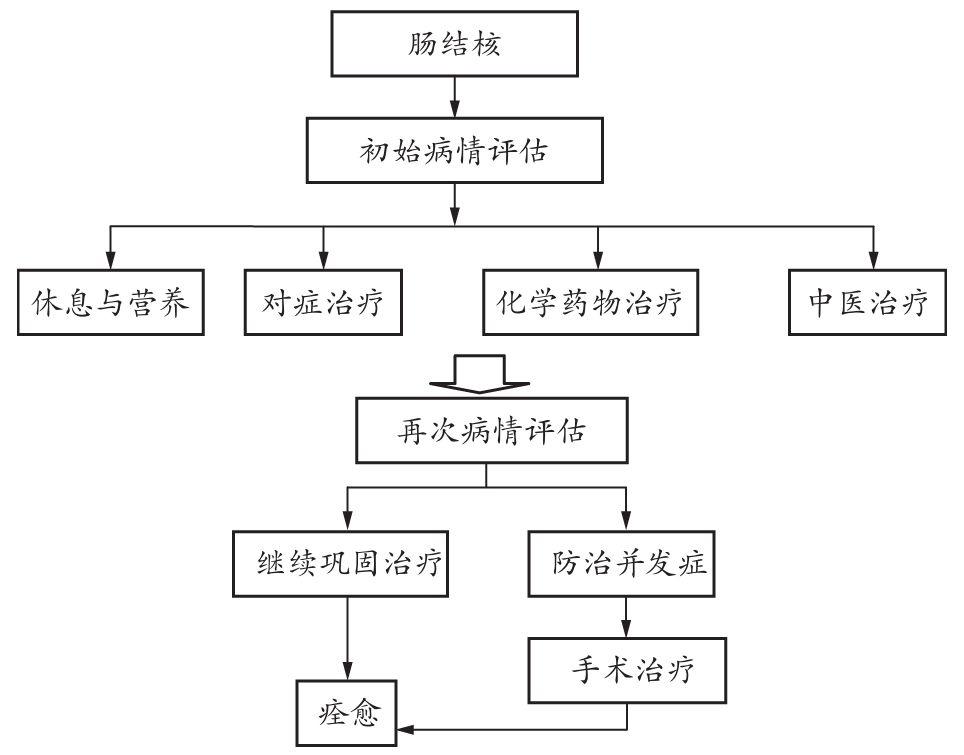
\includegraphics{./images/Image00090.jpg}
 \captionsetup{justification=centering}
 \caption{肠结核的治疗程序}
 \label{fig3-5-1}
  \end{figure} 

【治疗方案】 治疗原则 ①充分休息、合理营养、补充维生素,供给丰富的磷、钙、铁食物。②早期用药,坚持联合、足量、规律、全程抗结核药物治疗。③并发症治疗,不完全性肠梗阻、肠穿孔、肠出血等。④必要时手术治疗。

1.
一般治疗 合理的休息与营养应作为治疗结核的基础。活动性肠结核伴有急性渗出、溃疡形成时,应强调卧床休息,减少热量消耗,改善营养,增加机体抗病能力。活动性肠结核待病情稳定后,强调早期进行腹部的按摩、理疗促进肠管蠕动,避免肠管粘连,预防肠梗阻的发生。

2.
抗结核化学药物治疗 是本病治疗的关键。抗结核化学药物的选择、用法、疗程详见肺结核病。一般可分长疗程法与短疗程法:

(1)长疗程法:此系标准疗法,用异烟肼、链霉素两药或加对氨基水杨酸三药联合应用。全程需12\textasciitilde{}18个月。

(2)短疗程法:疗程缩短至6\textasciitilde{}9个月,其疗效与复发率和长疗程法取得同样满意效果。一般用异烟肼和利福平二种杀菌剂联合,对严重肠结核或伴有严重肠外结核者,宜加链霉素或吡嗪酰胺或乙胺丁醇三药联合。此种短疗程法需注意药物对肝脏的损害。可用利福啶代替利福平,每日150mg,毒性似较利福平为低。

WHO推荐的未获得(或缺乏)药敏试验结果但临床考虑MDR-TB时,可使用的化疗方案为强化期使用AMK(或CPM)+TH+PZA+OFLX联合,巩固期使用TH+OFLX联合。强化期至少3个月,巩固期至少18个月,总疗程21个月以上。

若化疗前或化疗中已获得了药敏试验结果,可在上述药物的基础上调整,保证敏感药物在3种以上。

3.
对症治疗 腹痛可用抗胆碱能药物。摄入不足或腹泻严重者应注意纠正水、电解质与酸碱平衡紊乱。对不完全性肠梗阻患者,需进行胃肠减压。

4.
中医中药治疗 根据患者的具体情况采用中医辨证施治。不完全性肠梗阻需行胃肠减压,同时可以利用承气汤加减进行直肠点滴给药。

5.
手术治疗 适应证包括:①完全性肠梗阻;②急性肠穿孔,或慢性肠穿孔瘘管形成经内科治疗而未能闭合者;③肠道大量出血经积极抢救不能有效止血者;④诊断困难需剖腹探查者。

【疗效观察与随访】

1. 观察指标

(1)临床症状、体征:观察发热、消瘦、腹痛、腹泻、便秘及腹部包块等的变化。

(2)实验室指标:溃疡型肠结核可有轻至中度贫血,无并发症时白细胞计数一般正常。血沉多明显增快,可作为观察结核病活动程度的指标之一。溃疡型肠结核的粪便多为糊样,显微镜下可见少量脓细胞与红细胞,隐血试验阳性。结核菌素试验呈强阳性有助本病诊断。

(3)X线检查:X线小肠钡剂造影在溃疡型肠结核,钡剂于病变肠段呈现激惹征象,排空很快,充盈不佳,而在病变的上、下肠段则钡剂充盈良好,称为X线钡影跳跃征象。病变肠段如能充盈,则显示粘膜皱襞粗乱、肠壁边缘不规则,有时呈锯齿状,可见溃疡。也可见肠腔变窄、肠段缩短变形、回肠盲肠正常角度消失。

(4)结肠镜检查:直接观察全结肠、盲肠及回盲部的病变,并可行活检或取样作细菌培养。内镜下见病变肠粘膜充血、水肿,溃疡形成(常呈横形、边缘呈鼠咬状),大小及形态各异的炎症息肉,肠腔变窄等。镜下取活体组织送病理检查具有确诊价值。

(5)并发症:①肠梗阻:是本病最常见的并发症,主要发生在增生型肠结核。溃疡型肠结核由于邻近腹膜粘连使肠曲遭受牵拉、束缚和压迫,或因肠溃疡愈合而有瘢痕收缩,可使肠腔狭窄引起梗阻。梗阻多系慢性进行性,程度轻重不等,迁延时间较长。少数可发展为完全性肠梗阻。②肠穿孔:发生率次于肠梗阻,居第二位,主要为亚急性或慢性穿孔,急性穿孔较少见,常发生在梗阻近端极度扩张的肠曲,或见于有多段肠狭窄造成的闭锁性肠梗阻。溃疡型肠结核虽有肠曲周围组织粘连,溃疡一般不穿破进入游离腹腔,但在病情发展快,机体反应差时,溃疡可向深部穿透,引起急性穿孔。③其他:有腹膜炎、肠粘连、肠套叠和憩室等。

2. 疗效评价

(1)治愈:全身及消化道症状及右下腹部压痛、腹块消失,大便正常。

(2)好转:血沉正常,纤维肠镜及钡灌肠显示肠道正常,临床症状改善。

(3)未愈:全身中毒症状无改善,血沉加快,甚至出现并发症如肠梗阻,水电解质、酸碱平衡失调。

3. 随访 半年内定期复查血沉、腹部B超,必要时做放射线复查或结肠镜检查。

【治疗经验与解析】

1.
抗结核化学药物治疗要遵循早期、联合、适量、规律、全程的原则,避免复发,防止并发症的发生。由于临床上患者对抗结核药物耐受性不同,肝肾功能情况不同(尤其是老年患者)和存在耐多药结核(MDR-TB)患者,治疗时要注意化疗方案制定的个体化,以确保化疗顺利完成。

2.
在选择药物联合治疗方案时应考虑药物的毒性反应。在服药期间应定期进行常规血清学、肝功能、肾功能试验,以及视觉、听力等相关检查。此外尚应密切观察临床表现,有时上述检查结果正常并不说明没有毒性反应。若服药期间发现有不良反应时应立即停药观察,并采取相应对症治疗措施。

3. 应做好本病与下列疾病的鉴别诊断

(1)克罗恩病:本病的临床表现和X线征象与肠结核极为酷似,有时甚难鉴别,下列几点协助诊断:①本病无肺结核或肠外结核病史。②病程一般更长,不经抗结核治疗可出现间断缓解。③粪便及其他体液及分泌物检查无结核菌。④X线检查可见病变以回肠末端为主,有多段肠曲受累,并呈节段性分布。⑤肠梗阻、粪瘘等并发症较肠结核更为多见。⑥切除病变肠段作病理检查无干酪样坏死,镜检与动物接种均无结核杆菌。

(2)右侧结肠癌:下列几点有助于鉴别诊断:①本病发病年龄多为40岁以上中老年人。②无长期低热、盗汗等结核症及结核病史。③病情进行性加重,消瘦、苍白、无力等全身症状明显。④腹部肿块开始出现时移动性稍大且无压痛,但较肠结核肿块表面坚硬,结节感明显。⑤X线检查主要有钡剂充盈缺损,病变局限,不累及回肠。⑥肠梗阻较早、较多出现。⑦纤维结肠镜检可窥见肿瘤,活检常可确诊。在临床上结肠癌的发病率较肠结核为高。

(3)阿米巴或血吸虫病性肉芽肿:该类疾病无结核病史,脓血便较常见,粪便中发现有关的病原体,直肠及结肠镜常可证实诊断,相应的特异性治疗有效。

(4)其他:以腹痛、腹泻为主要表现者应与腹型淋巴瘤、肠放线菌病相鉴别;以急性右下腹剧痛为主要表现者应注意避免误诊为急性阑尾炎;以慢性腹痛牵扯上腹部者易与消化性溃疡、慢性胆囊炎混淆;有稽留高热者需排除伤寒。

4.
复治患者应做药敏试验,对于所用方案化疗无效的复治排菌病例可参考耐多药肺结核化疗方案并根据药敏试验加以调整。对久治不愈的患者要警惕非结核分枝杆菌感染的可能性。

5.
饮食以高蛋白、糖类、维生素类为主,宜食新鲜蔬菜、水果及豆类。应戒烟禁酒。近年来研究证明,吸烟会使抗结核药物的血浓度降低,对治疗肺结核不利,饮酒能增加抗结核药物对肝脏的毒性作用,导致药物性肝炎。

6.
本病的预防应着重肠外结核特别是肺结核的早期诊断与积极治疗,使痰菌尽快转阴。肺结核患者不可吞咽痰液,应保持排便通畅,并提倡用公筷进餐,牛奶应经过灭菌。儿童应按时接种卡介苗。接种后可增加免疫力,卡介苗不能降低肺结核的发病率,但可以减轻发病后结核杆菌所造成的损害,提高自愈的可能,同时卡介苗最明显的作用就是显著减少了肺外结核的发病。患者应养成分食制习惯,与患者共餐或食入被结核杆菌污染的食物可引起消化道感染。

\subsection{结核性腹膜炎}

结核性腹膜炎(tuberculous
peritonitis)是由结核分枝杆菌引起的慢性弥漫性腹膜感染,其途径以腹腔内的结核病灶直接蔓延为主,肠系膜淋巴结结核、输卵管结核、肠结核等为常见的原发病灶,少数由血行播散引起。临床表现因病理类型及机体反应性的不同而异,主要有发热、腹痛、腹胀、腹水等。一般起病缓慢,早期症状较轻;少数起病急骤,以急性腹痛或骤起高热为主要表现。病理分为渗出、粘连、干酪三型,前两型较多见。本病可见于任何年龄,以中青年多见,男女之比约为1∶2。

【治疗程序】 如图\ref{fig3-5-2}所示。

\begin{figure}[!htbp]
 \centering
 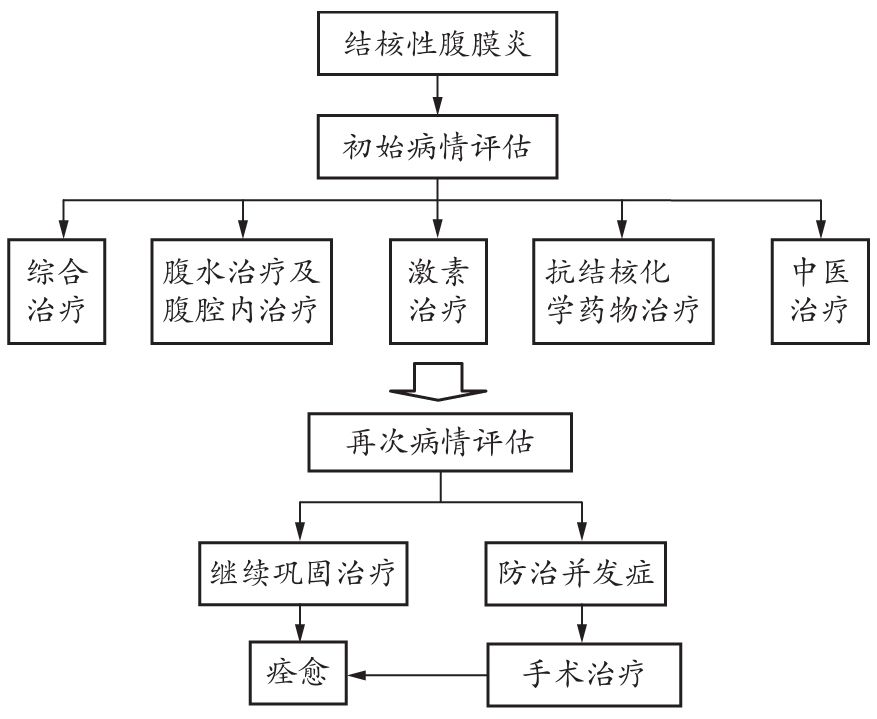
\includegraphics{./images/Image00091.jpg}
 \captionsetup{justification=centering}
 \caption{结核性腹膜炎的治疗程序}
 \label{fig3-5-2}
  \end{figure} 

【治疗方案】

1.
综合治疗 合理的休息与营养应作为治疗结核的基础。给予高热量、高蛋白、高维生素饮食。营养不良、消瘦患者适当用脂肪乳剂和氨基酸静脉内高营养治疗以增加机体能量。注意纠正水和电解质失衡。若伴有腹腔内混合其他细菌感染时应酌情给予抗生素治疗等。

2.
抗结核化学药物治疗 肺结核治疗的原则适用于结核性腹膜炎的治疗。抗结核化学药物的选择、用法、疗程详见肺结核。结核性腹膜炎的治疗通常需采用至少两种以上药物联合方案进行。在治疗前最好能对所分离的结核杆菌进行药物敏感试验,可进一步提高疗效。

对一些具有对结核杆菌耐药危险因素的患者,需要采用3种或4种抗结核药物联合治疗。这些危险因素有:①既往曾接受过抗结核药物的治疗。②未完成原定抗结核治疗方案、不规则用药、或疗程不足。③来自一些原发耐药结核杆菌株发生率超过50\%的地区患者,或与其密切接触者。④伴有HIV感染的患者。⑤患粘连型伴渗出或干酪型结核性腹膜炎的患者。⑥伴有其他部位活动性结核病灶,病变不易控制的患者等。

复发患者的处理:短期规律用药后自行停药而复发者,应在严格督导下原方案治疗9个月;用较简易方案或无规律用药而复发者,则需另定方案。

3.
腹水的处理 对腹水型患者如有大量腹水,可适当放腹水以减轻症状,在放腹水后,于腹腔内注入链霉素、醋酸可的松等药物,每周1次,可以加速腹水吸收并减少粘连。

4.
糖皮质激素治疗 在结核性腹膜炎抗结核治疗中加用适量糖皮质激素可减少中毒症状,减少炎性渗出和反应,并可减轻腹腔内纤维化或肠粘连的形成。因此结核中毒症状严重或腹腔内有大量渗出液的患者,在采用抗结核强化治疗同时可加用适量糖皮质激素治疗。

5. 中医中药治疗 根据患者的具体情况采用中医辨证施治。

6.
手术治疗 适应证包括:①并发完全性肠梗阻或有不全性肠梗阻经内科治疗而未见好转者。②急性肠穿孔,或腹腔脓肿经抗生素治疗未见好转者。③肠瘘经抗结核化疗与加强营养而未能闭合者。④本病诊断有困难,与急腹症不能鉴别时,可考虑剖腹探查。

【疗效观察与随访】

1. 观察指标

(1)观察患者发热、腹痛、腹胀及腹部体征的变化。

(2)观察实验室指标:如血象、腹水检查、病原学检查等。

(3)观察器械检查的变化:如腹部B超、胃肠X线检查、腹腔镜检查等。

(4)并发症:以肠梗阻为常见,多发生在粘连型。肠瘘一般多见于干酪型,往往同时有腹腔脓肿形成。

2. 治愈标准 症状、体征消失,各项相关检查正常,半年内无复发。

3. 随访 半年内定期复查腹部B超、腹水常规,密切观察病情变化。

【治疗经验与解析】

1.
在结核性腹膜炎治疗中,对一般渗出型病例,由于腹水及症状消失常不需太长时间,患者可能会自行停药,而导致复发,故必须强调全程规则治疗。对粘连型或干酪型病例,由于大量纤维增生,药物不易进入病灶达到应有浓度,病变不易控制,必要时宜考虑加强抗结核化疗的联合应用及适当延长抗结核的疗程。由于结核杆菌增殖缓慢和代谢失活的周期较长,所以延长药物治疗时间常是十分必要的。

2.
选择药物联合治疗方案时应考虑药物的毒性反应。在服药期间应定期进行常规血清学、肝功能、肾功能试验,以及视觉、听力等相关检查。此外尚应密切观察临床表现,有时上述检查结果正常并不说明没有毒性反应。若服药期间发现有不良反应时应立即停药观察,并采取相应对症治疗措施。

3.
选用糖皮质激素配合治疗,必须慎重,严格掌握应用指征和注意用药方法及剂量。

\section{炎症性肠病}

\subsection{溃疡性结肠炎}

溃疡性结肠炎(ulcerative
colitis,UC)是一种病因尚不十分清楚的直肠和结肠慢性非特异性炎症性疾病。病变主要限于大肠粘膜与粘膜下层。临床表现为腹泻、粘液脓血便、腹痛。病情轻重不等,多呈反复发作的慢性病程。本病可发生在任何年龄,多见于20\textasciitilde{}40岁,亦可见于儿童或老年。男女发病率无明显差别。本病在我国较欧美少见,且病情一般较轻,但近年患病率有明显增加,重症也常有报道。

【治疗程序】 如图\ref{fig3-6-1}\footnote{SASP:柳氮磺胺吡啶;5-ASA:5-氨基水杨酸;ACTH:促肾上腺皮质激素}所示。

\begin{figure}[!htbp]
 \centering
 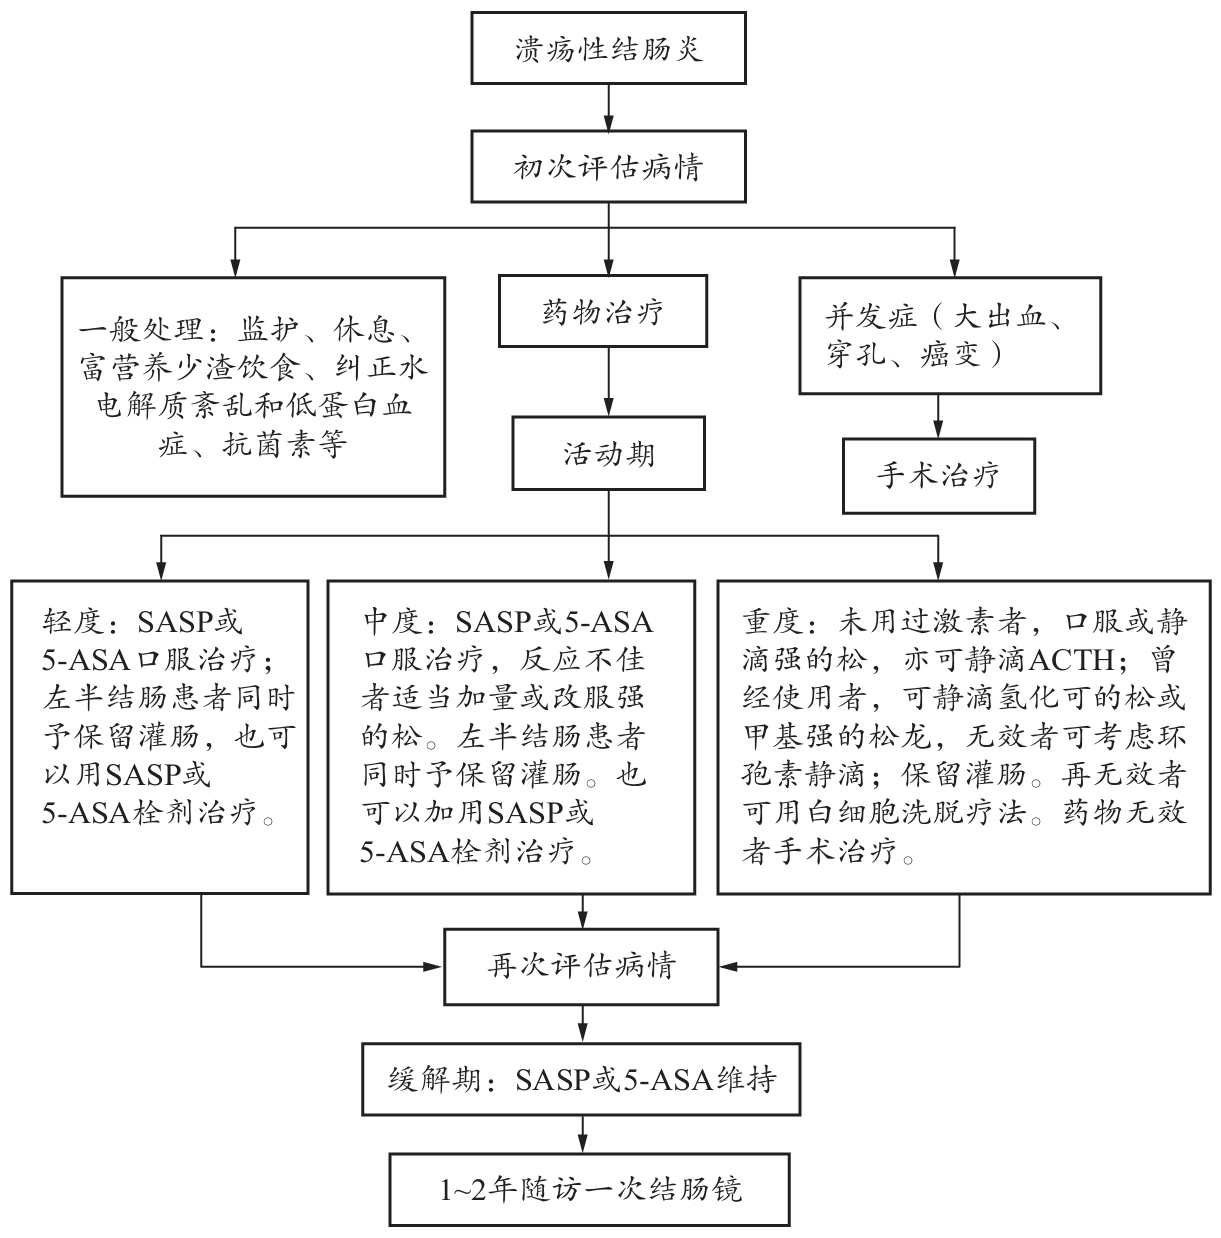
\includegraphics{./images/Image00092.jpg}
 \captionsetup{justification=centering}
 \caption{溃疡性结肠炎的治疗程序}
 \label{fig3-6-1}
  \end{figure} 


【治疗方案】

1. 治疗原则

(1)确定UC的诊断:首先排除各种有因可查的结肠炎;对疑诊病例可按UC治疗,进一步随诊,但先不用糖皮质激素。

(2)掌握好分级、分期、分段治疗的原则:分级是指按疾病的严重度,采用不同药物和不同治疗方法;分期指疾病分为活动期和缓解期,活动期以控制炎症及缓解症状为主要目标,缓解期应继续维持缓解,预防复发;分段治疗指确定病变范围以选择不同给药方法,远段结肠炎可采用局部治疗,广泛性结肠炎或有肠外症状者则以系统性治疗为主。溃疡性直肠炎治疗原则和方法与远段结肠炎相同。

(3)根据病程和过去治疗情况:确定治疗药物、方法及疗程,尽早控制发作,防止复发。

(4)注意:注意并发症,确定治疗终点及选择治疗方法。注意药物治疗过程中的不良反应。注意全身情况,评估预后及生活质量。

(5)综合性治疗:监护、休息、富营养少渣饮食、纠正水电解质紊乱和低蛋白血症、广谱抗菌素治疗、心理及对症处理等,内、外科医生会诊以确定内科治疗的限度和进一步处理方法。

2. 一般治疗 主要指内科治疗。

(1)活动期的治疗:

轻度UC:可选用柳氮磺胺吡啶(SASP),每日3\textasciitilde{}4g,分次口服;或用相当剂量的5-氨基水杨酸(5-ASA)。病变位于远段结肠者可用SASP或5-ASA栓剂0.5\textasciitilde{}1g,每日2次;5-ASA灌肠液1\textasciitilde{}2g或氢化可的松琥珀酸钠盐灌肠液100\textasciitilde{}200mg,每晚1次保留灌肠;有条件者可用布地奈德2mg保留灌肠,每晚1次;亦可用中药保留灌肠。

中度UC:可用上述剂量水杨酸类制剂治疗,反应不佳者适当加量或改服糖皮质激素,常用泼尼松30\textasciitilde{}40mg/d口服。

重度UC:重度UC须及时处理,足量给药,治疗方法如下:①未曾使用过口服糖皮质激素患者,可口服泼尼松或泼尼松龙40\textasciitilde{}60mg/d,观察7\textasciitilde{}10日,亦可直接静脉给药;已使用糖皮质激素者,应静脉滴注氢化可的松300mg/d或甲基泼尼松龙48mg/d。②肠外应用广谱抗生素如硝基咪唑、喹诺酮类制剂、氨苄青霉素或头孢类等抗生素控制肠道继发感染。③患者应卧床休息,适当输液、补充电解质。④便血量大、Hb\textless{}90g/L和持续出血不止者应考虑输血。⑤营养不良、病情较重者可用要素饮食,病情严重者应予肠外营养。⑥静脉糖皮质激素使用7\textasciitilde{}10日后无效者,可考虑环孢素2\textasciitilde{}4mg/(kg·d)静脉滴注7\textasciitilde{}10日,监测血药浓度,注意不良反应。顽固性UC亦可考虑用其他免疫抑制剂,如硫唑嘌呤(Aza)1.5\textasciitilde{}2.5mg/(kg·d)、6-巯基嘌呤(6-MP)0.75\textasciitilde{}1.5mg/(kg·d)等,不能耐受者可改为甲氨蝶呤(MTX)每周15\textasciitilde{}25mg,肌内注射,或参考药典和教科书。⑦上述治疗无效者在条件允许的医疗单位可采用白细胞洗脱疗法。⑧如上述药物疗效不佳,应及时内、外科会诊,确定结肠切除手术的时机和方式。⑨慎用解痉剂及止泻剂,以避免诱发中毒性巨结肠。⑩密切监测患者生命体征和腹部体征变化,尽早发现和处理并发症。

(2)缓解期的治疗:除初发病例、轻症远段结肠炎患者症状完全缓解后可停药观察外,所有患者完全缓解后均应继续维持治疗。SASP的维持治疗剂量一般为控制发作之半,多用2\textasciitilde{}3g/d,并同时口服叶酸;亦可用相同剂量的5-ASA类药物。糖皮质激素无维持治疗效果,在症状缓解后应逐渐减量,过渡至用5-ASA维持治疗。6-MP或Aza等用于上述药物不能维持或对糖皮质激素依赖的患者。

(3)其他治疗:①5-ASA与免疫抑制剂均无效者,可用新型生物治疗剂,如抗肿瘤坏死因子-a(TNF-a)单克隆抗体。②益生菌维持治疗。③根据辨证施治原则,适当选用中药方剂中具抗炎、止泻、粘膜保护、抑制免疫反应的药物等替代治疗,多种中药灌肠制剂也有一定的疗效。④治疗中对患者加强教育,提高治疗依从性、早期识别疾病发作与定期随访。

3. 外科手术治疗

(1)绝对指征:大出血、穿孔、明确或高度怀疑癌肿及组织学检查发现重度异型增生或肿块性损害轻、中度异型增生。

(2)相对指征:重度UC伴中毒性巨结肠、静脉用药无效者;内科治疗症状顽固、体能下降、对糖皮质激素抵抗或依赖的顽固性病例,替换治疗无效者;UC合并坏疽性脓皮病、溶血性贫血等肠外并发症者。

【疗效观察与随访】

1. 观察指标

(1)症状、体征:观察治疗前后腹泻、粘液脓血便腹痛等消化系统症状和腹部体征的变化。

(2)肠外表现:观察治疗前后发热、消瘦、贫血、低蛋白血症、水与电解质平衡紊乱等全身表现及外周关节炎、巩膜外层炎、前葡萄膜炎等肠外表现的变化。

(3)并发症:观察有无中毒性巨结肠、肠出血、肠穿孔及肠梗阻等并发症。

(4)血液检查:血红蛋白在轻型病例多正常或轻度下降,中、重型病例有轻或中度下降,甚至重度下降。白细胞计数在活动期可有增高。血沉加快和C-反应蛋白增高是活动期的标志。严重病例血清白蛋白下降。

(5)粪便检查:主要为常规检查及病原学检查。

(6)结肠镜检查:是本病诊断、鉴别诊断及疗效观察的最重要手段之一。作全结肠及回肠末段检查,直接观察肠粘膜变化,取活组织检查,并确定病变范围。本病病变呈连续性、弥漫性分布,从肛端直肠开始逆行向上扩展。

(7)X线钡剂灌肠检查:有重要价值,可观察病情变化。

2. 治愈标准 症状、体征消失,相关检查正常,半年内无复发。

3.
随访 癌变的监测:对病程8\textasciitilde{}10年以上的广泛性结肠炎、全结肠炎和病程30\textasciitilde{}40年以上的左半结肠炎、直乙状结肠炎患者,UC合并原发性硬化性胆管炎者,至少两年1次结肠镜检查,并作多部位活检。对组织学检查发现有异型增生者,应密切随访,如为重度异型增生,一经确认即应手术治疗。

【治疗经验与解析】

1.
本病是一种慢性病,需要长期治疗,营养与饮食的调配很重要。腹泻常伴有脂肪吸收不良,应限制脂肪和膳食纤维摄入。

2.
本病呈慢性反复发作过程,应密切注意中毒性巨结肠、肠出血、肠穿孔等并发症的发生,并及时作出相应处理;尤其病程漫长者癌变危险性增加,应密切随访。

\subsection{克罗恩病}

克罗恩病(Crohn's
disease,Crohn病,CD)是一种病因尚不十分清楚的胃肠道慢性炎性肉芽肿性疾病。病变多见于末段回肠和邻近结肠,但从口腔至肛门各段消化道均可受累,呈节段性或跳跃式分布。克罗恩病的根本原因未明,目前认为本病可能系感染、免疫反应、遗传多种因素的综合作用的结果。临床上以腹痛、腹泻、体重下降、腹部肿块、瘘管形成和肠梗阻为特点,可伴有发热等全身表现以及关节、皮肤、眼、口腔粘膜等肠外损害。本病有终身复发倾向,重症患者迁延不愈,预后不良。本病的典型病理组织学改变是非干酪性肉芽肿。发病年龄多在15\textasciitilde{}30岁,但首次发作可出现在任何年龄组,男女患病率近似。本病在欧美多见,且有增多趋势。我国本病发病率不高,但并非罕见。

【治疗程序】 如图\ref{fig3-6-2}\footnote{SASP:柳氮磺胺吡啶;5-ASA:5-氨基水杨酸}所示。

\begin{figure}[!htbp]
 \centering
 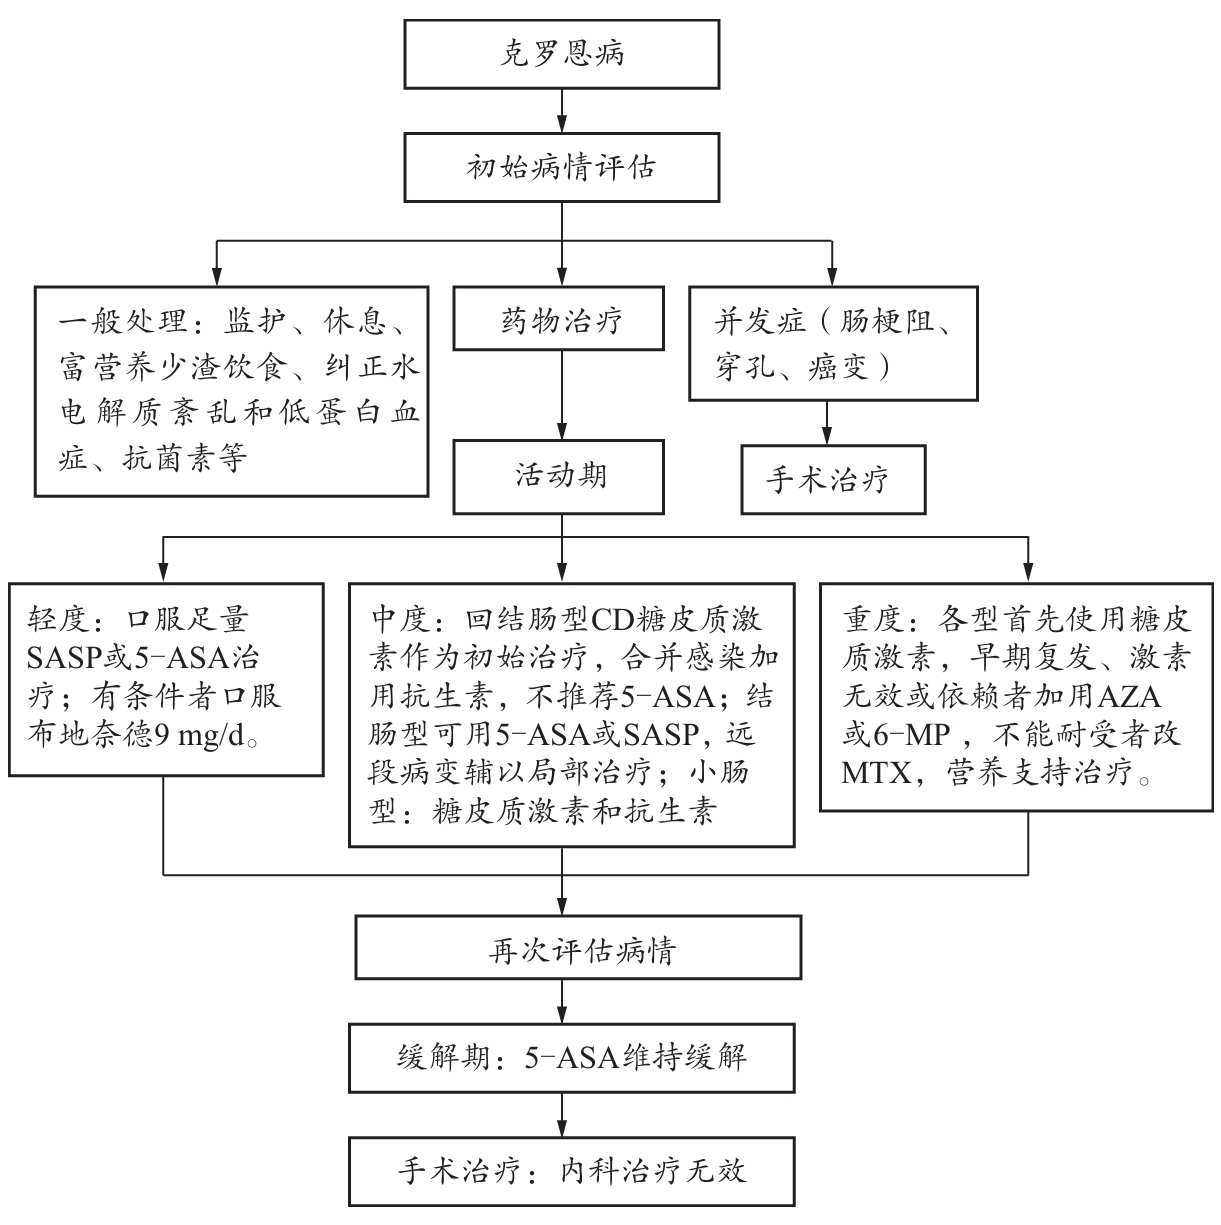
\includegraphics{./images/Image00093.jpg}
 \captionsetup{justification=centering}
 \caption{克罗恩病的治疗程序}
 \label{fig3-6-2}
  \end{figure} 

【治疗方案】

1.
一般治疗 所有CD患者必须戒烟;注意营养支持、对症及心理治疗的综合应用。对重症患者均应采用营养支持治疗,可酌用要素饮食或全胃肠外营养,以助诱导缓解。

2. 活动期的治疗

(1)回结肠型CD:①轻度:口服足量SASP或5-ASA作为初始治疗,有条件者口服布地奈德9mg/d。②中度:糖皮质激素作为初始治疗,也可用布地奈德,合并感染加用抗生素,如环丙沙星500\textasciitilde{}1000mg/d,或10\textasciitilde{}20mg/(kg·d)或甲硝唑800\textasciitilde{}1200mg/d。不推荐5-ASA。③重度:首先使用糖皮质激素,用法同重度UC治疗。

早期复发、激素治疗无效或激素依赖者需加用Aza1.5\textasciitilde{}2.5mg/(kg·d)或6-MP0.75\textasciitilde{}1.5mg/(kg·d)。不能耐受者可改为甲氨蝶呤(MTX)每周15\textasciitilde{}25mg,肌内注射,或参考药典和教科书。上述药物治疗无效或不能耐受者有条件可用英夫利昔单抗(infliximab)5\textasciitilde{}10mg/kg,控制发作一般需静脉滴注3次。

(2)结肠型CD:①轻、中度:可选用5-ASA或SASP,亦可开始即使用糖皮质激素。远段病变可辅以局部治疗。②重度:药物选择同重度回结肠型CD。

(3)小肠型CD:①轻度:回肠病变可用足量控释5-ASA;广泛性小肠CD营养治疗作为主要治疗方案。②中、重度:使用糖皮质激素(布地奈德最佳)和抗生素,推荐加用Aza或6-MP,不能耐受者可改为MTX。营养支持治疗则作为重要辅助治疗措施。上述治疗无效,则考虑英夫利昔或手术治疗。

(4)其他:累及胃、十二指肠者治疗与小肠型CD相同,加用质子泵抑制剂;肛门病变,如肛瘘时抗生素为第一线治疗,Aza、6-MP、英夫利昔对活动性病变有良效,或加用脓肿引流、皮下置管等;其他部位瘘管形成者治疗与上述中、重度的诱导缓解方案相同,亦可考虑英夫利昔与手术治疗,具体方案需因人而异。

3.
缓解期的治疗 首次药物治疗取得缓解者,可用5-ASA维持缓解,药物剂量与诱导缓解的剂量相同;频繁复发及病情严重者在使用糖皮质激素诱导缓解时,应加用Aza或6-MP,并在取得缓解后继续以Aza或6-MP维持缓解,不能耐受者可改用小剂量MTX;使用英夫利昔诱导缓解者推荐继续定期使用以维持缓解。维持缓解治疗用药时间一般为3\textasciitilde{}5年甚至更长。

4.
其他治疗 新型生物治疗剂的应用;益生菌维持治疗;中药辨证施治,方剂中不乏抗炎、止泻、粘膜保护、抑制免疫反应药物,作为替换治疗的重要组成部分。

5.
外科治疗 是CD治疗的最后选择,适用于积极内科治疗无效而病情危及生命或严重影响生存质量者、有并发症(穿孔、梗阻、腹腔脓肿等)需外科治疗者。

6.
术后复发的预防 CD病变肠道切除术后复发率相当高。患者术后原则上均应用药预防复发。一般选用5-ASA。硝基咪唑类抗生素有效,但长期使用不良反应多。易于复发的高危患者可考虑使用Aza或6-MP。预防用药推荐在术后2周开始,持续时间不少于2年。寻找有效措施预防复发仍是当今研究的热点。小肠CD炎症部位可能并发癌肿,但不发生于结肠;结肠CD癌变危险性与UC相近,监测方法相同。

【疗效观察与随访】

1. 观察指标

(1)症状、体征:治疗前后右下腹或脐周腹痛、腹泻、腹部肿块、梗阻、肠瘘、肛门病变的变化,及发热、贫血、体重下降、发育迟缓等全身症状的变化。

(2)影像学检查:胃肠钡剂造影,必要时结合钡剂灌肠。可见多发性、跳跃性病变,呈节段性炎症伴僵硬、狭窄、裂隙状溃疡、瘘管、假息肉及鹅卵石样改变等。腹部超声、CT、MRI可显示肠壁增厚、腹腔或盆腔脓肿、包块等。

(3)肠镜检查及活检:结肠镜应达末段回肠。可见节段性、非对称性的粘膜炎症、纵行或阿弗他溃疡、鹅卵石样改变,可有肠腔狭窄和肠壁僵硬等。病变肠段病理活检有助确诊,应多点活检,必要时应多次活检。

(4)胶囊内镜及双气囊小肠镜:对小肠病变的观察具有重大意义。

(5)常规实验室检查:粪便常规和必要的病原学检查、血常规、血浆蛋白、电解质、红细胞沉降率、C反应蛋白、腹部平片等。有条件的单位亦可作粪便钙卫蛋白、乳铁蛋白、α{1}
抗胰蛋白酶等检查。

(6)并发症:可有肠梗阻、瘘管、炎性包块或脓肿、出血、肠穿孔等。

(7)复发:CD病变肠道切除术后复发率相当高,术后应密切观察有无症状及体征的复发。

2. 治愈标准 症状、体征消失,相关检测指标正常,半年内无复发。

3.
随访 ①初发病例、临床与影像或内镜及活检改变难以确诊时,应随访观察3\textasciitilde{}6个月。②小肠CD炎症部位可能并发癌肿,结肠CD癌变危险性与UC相近,监测方法相同。

【治疗经验与解析】

1.
由于该病严重程度与活动性判断不如UC明确,临床缓解与肠道病变恢复常不一致;治疗效果不如UC,疾病过程中病情复杂多变。因而,治疗过程中应重视病情的观察和分析,更强调个体化的治疗原则。

2.
由于CD与肠结核症状、体征相似,常常难以鉴别,如与肠结核混淆不清者应按肠结核作诊断性治疗4\textasciitilde{}8周,以观后效。

3.
本病的治疗中应注重对患者的教育,提高治疗依从性、早期识别疾病发作与定期随访。

4.
该病病因迄今未明,可能与遗传、环境,饮食,感染等因素有关,吸烟似乎与克罗恩病的发展或恶化有关,治疗中应避免环境,饮食,感染等因素的影响,戒烟酒。

5.
由于缺乏典型临床表现及认识不充分,临床中极易误诊,延误治疗,导致严重的并发症,应引起临床医生重视。

6.
CD诊断应包括临床类型、严重程度(活动性、严重度)、病变范围、肠外表现和并发症,以利全面估计病情和预后,制订治疗方案。

7.
CD病变肠道切除术后复发率相当高,患者术后原则上均应用药预防复发。一般选用5-ASA。易于复发的高危患者可考虑使用Aza或6-MP。预防用药推荐在术后2周开始,持续时间不少于2年。

\section{大肠癌}

大肠癌包括结肠癌与直肠癌(colorectal
carcinoma),是胃肠道常见的恶性肿瘤。腹痛、排便习惯与粪便性状改变为本病最早出现的症状,并发症见于晚期,主要有肠梗阻、肠出血及肠穿孔。确诊依据结肠镜及组织病理检查。我国发病年龄多在40\textasciitilde{}60岁,发病高峰在50岁左右,比欧美提前约十年。男女发病率约为1.6∶1。我国大肠癌发病率上升趋势十分明显。

【治疗程序】 如图\ref{fig3-7-1}所示。

\begin{figure}[!htbp]
 \centering
 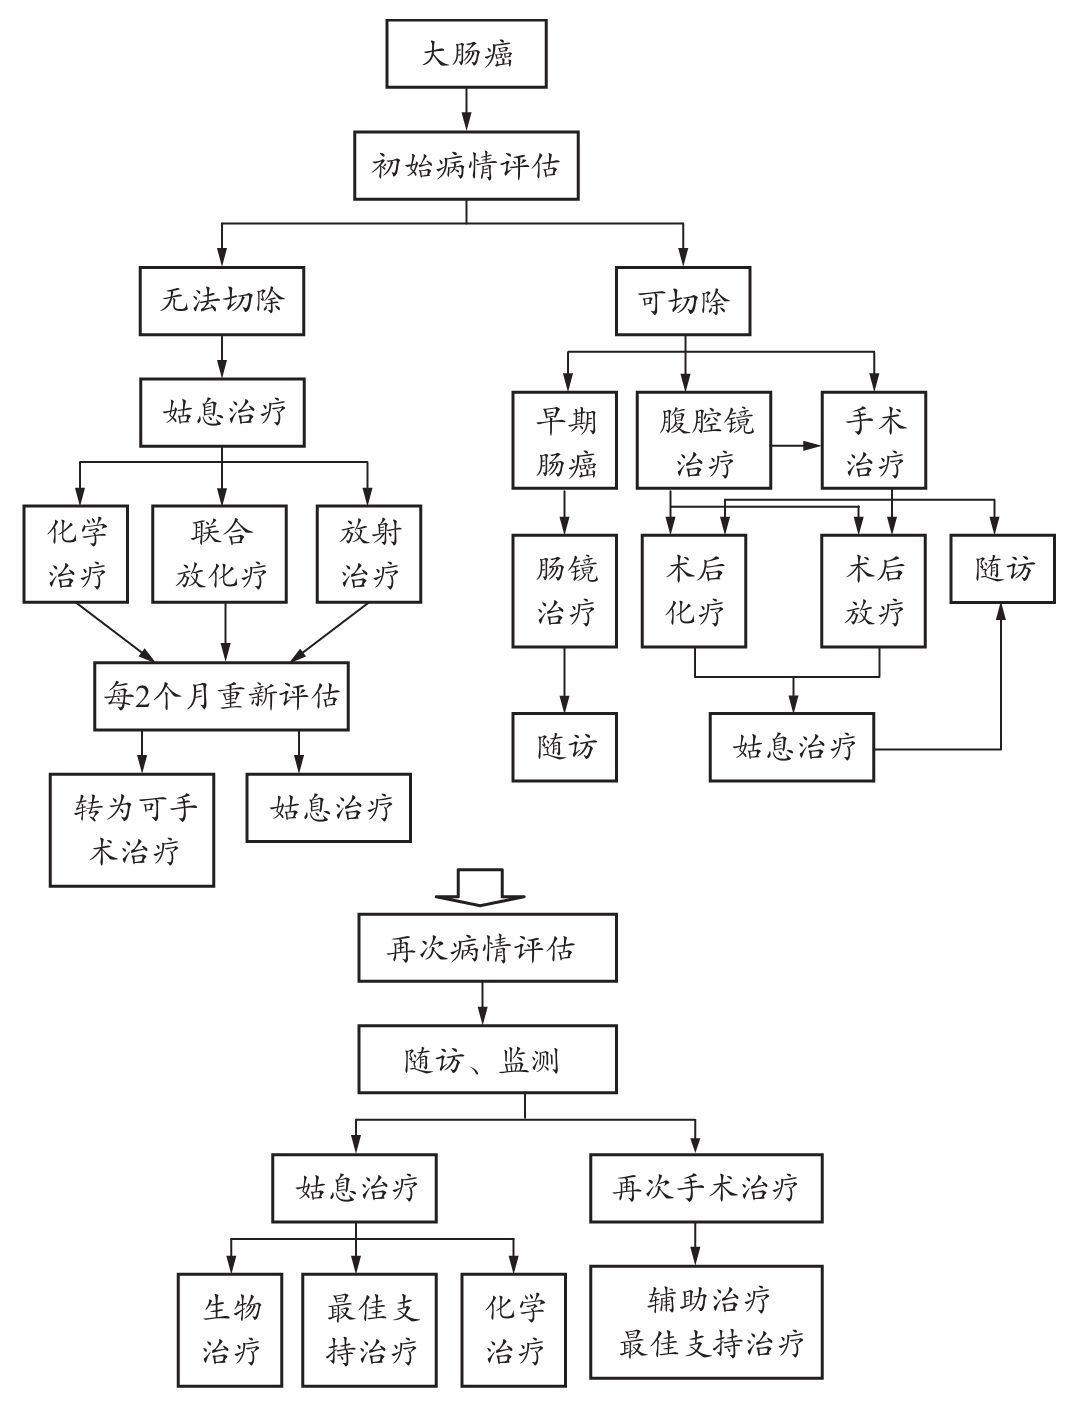
\includegraphics{./images/Image00094.jpg}
 \captionsetup{justification=centering}
 \caption{大肠癌的治疗程序}
 \label{fig3-7-1}
  \end{figure} 

【治疗方案】

1. 外科治疗

(1)结肠癌的唯一根治方法是癌肿的早期切除。对有广泛癌转移者,如病变肠段已不能切除,则应进行造瘘等姑息手术。结肠切除术的范围是要去除其主要的供应动脉血管及其相关的淋巴。对结肠同时性癌可以分别切除或结肠次全切除。结肠癌侵犯邻近器官时,如果一侧或双侧卵巢有明显异常增大或由于局部被结肠癌广泛侵袭时,建议行双侧卵巢切除。

(2)腹腔镜结肠手术:属微创手术,目前腹腔镜手术已可用于结肠的任何部位,包括结直肠良性和恶性病变,但对应用腹腔镜进行恶性肿瘤根治性切除,还有争议。其适应证和病例选择,主要取决于外科医生腹腔镜手术的经验。并非所有的病变均能用腹腔镜进行切除,如累及邻近器官的较大和晚期肿瘤,因肿瘤浸润或以往手术操作引起的严重粘连,肥胖患者也较难进行腹腔镜手术。

2.
经结肠镜治疗 结肠腺瘤癌变和粘膜内的早期癌可经结肠镜用高频电凝切除。切除后的息肉回收做病理检查,如癌未累及基底部则可认为治疗完成;如累及根部,需追加手术,彻底切除有癌组织的部分。对晚期结、直肠癌形成肠梗阻,患者一般情况差不能手术者,可经结肠镜用激光打通肿瘤组织,作为一种姑息疗法,可在内镜下放置支架,解除狭窄或梗阻。

3.
化学药物治疗 大肠癌对化学药物一般不很敏感,是一种辅助疗法。早期癌根治后一般不需化疗。氟尿嘧啶(5-FU)至今仍是大肠癌化疗的首选药物,常与其他化疗药如奥沙利铂等联合应用。临床上结肠癌的化疗方案用量及用法繁多,应遵循个体化的治疗原则。

腹腔内灌注化疗,目的是在肿瘤部位直接提高抗癌药浓度,增加局部细胞毒作用而不增加甚至减少或避免对全身的毒副作用。联合应用腹腔内灌注化疗和系统性静脉化疗的方法可提高疗效。

4.
放射治疗 用于直肠癌,术前放疗可提高手术切除率和降低术后复发率;术后放疗仅用于手术未达根治或术后局部复发者。单纯放疗,仅用于晚期直肠癌病例,有止血,镇痛、延长存活期的作用。结肠癌放射治疗的作用是有限的,放疗对于腹部脏器的潜在损伤限制了它在结肠癌治疗中的应用。

【疗效观察与随访】

1. 观察指标

(1)观察治疗后患者症状、体征的变化:①排便习惯与粪便性状改变常为本病最早出现的症状。多为血便,或有痢疾样脓血便伴里急后重,大便形状变细。有时表现为顽固性便秘,或腹泻与便秘交替。②腹痛是本病的早期症状,多见于右侧大肠癌。表现为右腹钝痛,或同时涉及右上腹、中上腹。大肠癌并发肠梗阻时腹痛加重或为阵发性绞痛。③腹部肿块位置取决于癌的部位。④多数直肠癌患者经指检可以发现直肠肿块,质地坚硬,表面呈结节状,有肠腔狭窄,指检后的指套上有血性粘液。

(2)观察有无并发症出现:①肠梗阻主要表现为腹痛,腹胀,肛门停止排气排便,呕吐等。大肠癌性梗阻70\%位于左半结肠,右半结肠梗阻仅占大肠癌性梗阻的20\%\textasciitilde{}30\%,其中30\%的左半结肠梗阻位于结肠肝区。②肠穿孔临床有典型的急腹症表现,腹肌紧张、压痛、反跳痛,X线平片见膈下新月状游离气体等,可作出初步的诊断。③急性大出血是大肠癌较少见的并发症。临床短时间内一次或反复多次大量鲜或暗红色血便,出血量往往超过1000ml以上,导致心率增快、血压下降、肝冷、尿量减少甚至休克等一系列症状,常危及生命。

(3)结肠镜检查:通过结肠镜能直接观察全大肠的肠壁、肠腔的改变,并确定肿瘤有无复发及肿瘤的部位、大小,初步判断浸润范围,取活检可获确诊。

(4)X线钡剂灌肠:最好采用气钡双重造影,可发现充盈缺损、肠腔狭窄、粘膜皱襞破坏等征象,显示癌肿部位和范围。对结肠镜检查因肠腔狭窄等原因未能继续进镜者,钡剂灌肠对肠镜未及肠段的检查尤为重要。

(5)其他影像学检查:电子计算机X线体层显像(CT)主要用于了解大肠癌肠外浸润及转移情况。超声结肠镜的应用可观察大肠癌在肠壁浸润深度及周围淋巴结转移情况。

(6)观察实验室检查:①粪便隐血检查方法简便易行,可提供早期诊断的线索。②血清癌胚抗原(CEA)测定:结肠癌患者70\%\textasciitilde{}90\%显示CEA高度阳性,血清CEA水平变化与结肠癌Duke分期密切相关。升高时主要见于中晚期肿瘤,进展期结肠癌(Duke分期C、D期)时阳性率可达70\%以上,而DukeA、B期时敏感性只有30\%左右。对于CEA升高的结肠癌患者,血清CEA水平与癌肿大小、有无转移存在一定关系,当发生肝转移时,CEA升高更为明显。放射免疫法检测CEA,作定量动态观察,对判断大肠癌的手术效果与监测术后复发有一定意义,如大肠癌经手术将肿瘤完全切除后,血清CEA则逐渐下降;若复发,又可再度升高。

2. 治愈标准 症状、体征消失,术后5年内未复发。

3.
随访 所有的大肠癌患者都应该接受系统性的随访。随访的内容包括全面的病史询问和体格检查,全血细胞、血CEA、肝肾功能、胸部X线、腹部B超或CT、PET、内窥镜检查等,前2年内每3\textasciitilde{}6个月进行1次上述全面检查,然后每6个月1次,共5年。肠镜的随访主张在术后3\textasciitilde{}6个月即行首次结肠镜检查,以防漏诊异时癌。

【治疗经验与解析】

1.
结肠癌早期症状多较轻或不明显,易被患者忽视和漏诊。对中年以上患者有下列表现时应警惕有无结肠癌的可能:①近期内出现排便习惯改变(如便秘、腹泻或排便不畅)、持续腹部不适、隐痛或腹胀;②粪便隐血试验持续阳性;③粪便变稀,或带有血液和粘液;④腹部可扪及肿块;⑤原因不明的贫血、乏力或体重减轻等。对有上述症状的患者及早进行X线钡剂灌肠或结肠镜检查,是早期诊断本病的关键。

2.
对40岁以上具有下列高危因素者:大肠腺瘤、有家族史如大肠息肉综合征或家族遗传性非息肉大肠癌或一级血缘亲属中有大肠癌者、溃疡性结肠炎等,应进行长期随访,定期肠镜检查。

3.
下列措施可减少大肠癌的发病率:①避免长期进食高脂食物,多进富含纤维的食物,保持大便通畅;②多食用新鲜蔬菜、水果、大蒜、茶叶等天然抑癌食品,适当补充维生素A、维生素B{12}
、维生素C、维生素D、维生素E和叶酸;③积极防治癌前病变,对有肠息肉,尤其是肠息肉家族遗传性患者,须及早予以切除;大力防治出血吸虫病及血吸虫肉芽肿;④对有癌瘤遗传易感性和癌瘤家族史的人群应定期行癌前普查;近期有进行性消瘦及大便习惯改变者,也应及早行有关检查,以期尽早发现;⑤对早期肠癌手术后或放疗后患者,应定期复查,有条件者应长期坚持给予扶正抗癌中药巩固治疗,预防复发。

4. 生物治疗尚在探索阶段,常用干扰素、白介素治疗。

\section{功能性胃肠病}

功能性胃肠病(functional gastrointestinal
disorder)是一组表现为慢性或反复发作性的胃肠道综合征,临床表现主要是胃肠道(包括咽、食管、胃、胆道、小肠、大肠、肛门)的相关症状。

\subsection{功能性消化不良}

功能性消化不良(functional
dyspepsia,FD)是指具有由胃和十二指肠功能紊乱引起的症状,经检查排除引起这些症状的器质性疾病的一组临床综合征。

根据临床特点,本病分为两个临床亚型:①上腹痛综合征(EPS):上腹痛和(或)上腹灼热感。②餐后不适综合征(PDS):餐后饱胀和(或)早饱。两型可有重叠。

【治疗程序】 如图\ref{fig3-8-1}所示。

\begin{figure}[!htbp]
 \centering
 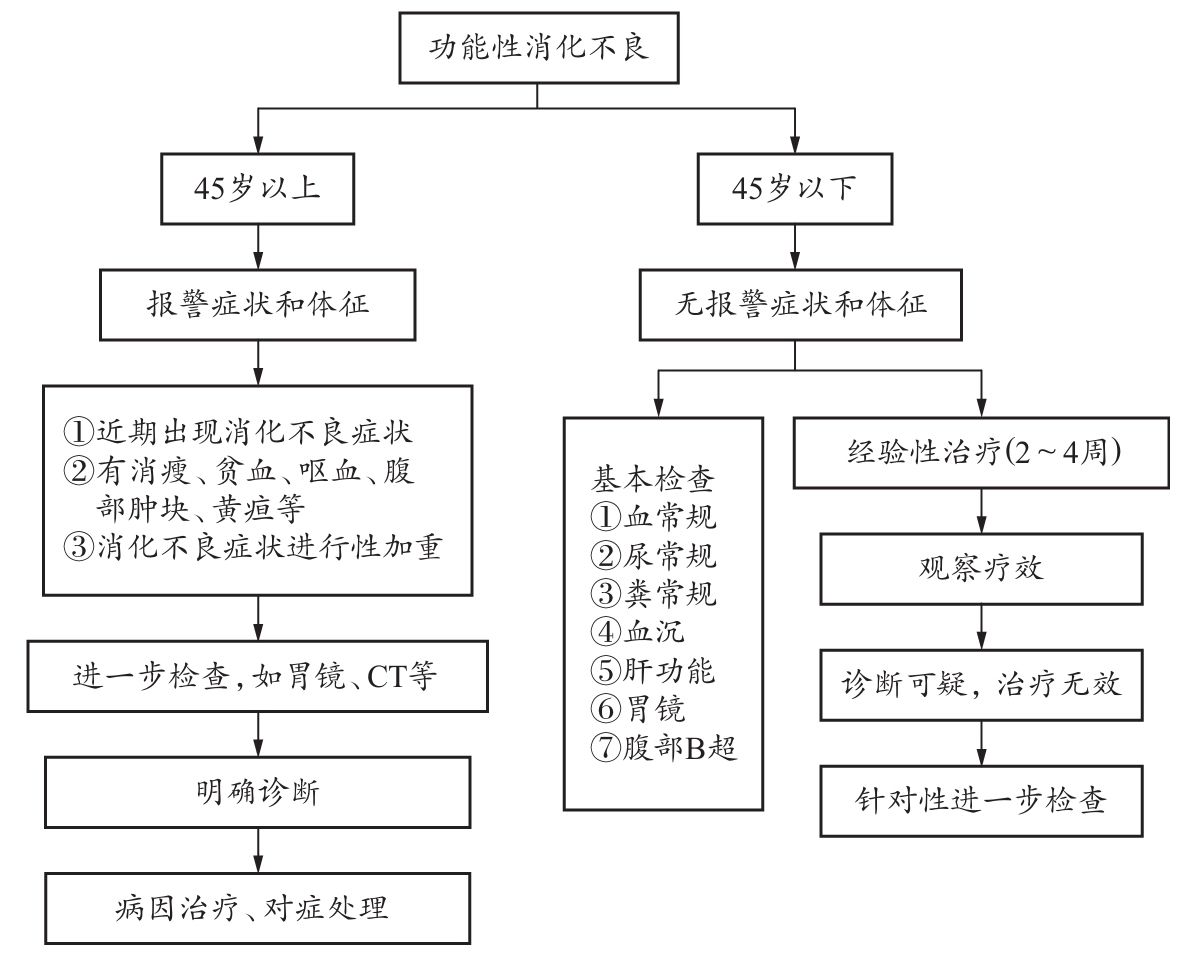
\includegraphics{./images/Image00095.jpg}
 \captionsetup{justification=centering}
 \caption{功能性消化不良的治疗程序}
 \label{fig3-8-1}
  \end{figure} 

【治疗方案】 主要是对症治疗,遵循综合治疗和个体化治疗的原则。

1.
一般治疗 建立良好的生活习惯,避免烟、酒及服用非甾体抗炎药。无特殊食谱,避免个人生活经历中会诱发症状的食物。注意根据患者不同特点进行心理治疗。失眠、焦虑者可适当予以镇静药。

2. 药物治疗 无特效药,主要是经验性治疗。

(1)抑制胃酸分泌药:一般适用于以上腹痛、上腹灼热感为主要症状的患者,可选择H{2}
受体拮抗剂或质子泵抑制剂。

(2)促胃肠动力药:一般适用于以餐后饱胀、早饱为主要症状患者。多潘立酮(每次10mg、每日3次)、莫沙必利(每次5mg、每日3次)或依托必利(每次50mg、每日3次)均可选用,甲氧氯普胺因长期服用不良反应大,现已少用于FD治疗。

对疗效不佳者,抑制胃酸分泌药和促胃肠动力药可换用或合用。

(3)根除幽门螺杆菌治疗:对小部分有幽门螺杆菌感染的FD患者可能有效,可试用。

(4)抗抑郁药:上述治疗疗效欠佳而伴随精神症状明显者可试用。常用的有三环类抗抑郁药如阿米替林、选择性抑制5-羟色胺再摄取的抗抑郁药如帕罗西汀等,宜从小剂量开始,注意药物的不良反应。

【疗效观察与随访】

1. 观察指标 报警症状与体征、腹部B超、胃肠内镜、CT、肝肾功能等。

2. 疗效判定

治愈标准 症状、体征消失,相关检查指标均为阴性。

好转标准 症状仍时有出现,但相关检查指标均为阴性。

3.
随访 对好转病例应密切观察病情,特别一旦出现报警症状与体征应及时诊治,必要时行全面检查。

【治疗经验与解析】

1.
需要与本病相鉴别的疾病包括:食管、胃和十二指肠的各种器质性疾病如消化性溃疡、胃癌等;各种肝胆胰疾病;由全身性或其他系统疾病引起的上消化道症状如糖尿病、肾脏病、结缔组织病及精神病等;药物引起的上消化道症状如服用非甾体类抗炎药;其他功能性胃肠病和动力障碍性疾病如胃食管反流病、肠易激综合征等。应注意,不少FD患者常同时有胃食管反流病、肠易激综合征及其他功能性胃肠病并存,临床上称之为症状重叠。

2.
消化不良是集中于上腹的慢性和复发性疼痛。主要或常出现(1周超过1次)烧心或酸反流的患者应考虑GERD,直至能证明其不是为止。年龄大于55岁,或有报警症状的消化不良患者应立即行内镜检查。其他患者有两种大致相等的治疗选择:①应用已确定有效的非侵入性检测方法进行幽门螺杆菌检测和治疗,如果根除成功而症状未解除则给予酸抑制治疗。②或经验性使用PPI作酸抑制治疗4\textasciitilde{}8周。检测和治疗更适于幽门螺杆菌感染中、高度流行的人群(≥10\%),而经验性PPI治疗是幽门螺杆菌低流行人群的首要选择。

如果2\textasciitilde{}4周后初始酸抑制失败,则考虑改变药物种类或剂量是合理的。如果患者对治疗无效应,或停止抗分泌治疗后迅速复发,则建议行内镜检查。目前并不推荐促动力药作为未调查消化不良的一线治疗药物。对于始终有症状的患者,内镜检查并不是必需的,因为其作用不大;是否行内镜检查必须根据临床判断。对初始治疗有效应的患者,4\textasciitilde{}8周后停止治疗;如果症状复发,则重复另一疗程相同的治疗。当初始抗分泌治疗和幽门螺杆菌根除失败时,功能性消化不良的治疗极具挑战性。极其有限的资料支持在功能性消化不良中应用低剂量三环类抗抑郁药或心理治疗。

\subsection{肠易激综合征}

肠易激综合征(irritable bowel
syndrome,IBS)是一种以腹痛或腹部不适伴排便习惯改变为特征的功能性肠病,经检查排除可引起这些症状的器质性疾病。最主要的临床表现是腹痛与排便习惯和粪便性状的改变。

【治疗方案】

1.
一般治疗 详细询问病史以求发现促发因素,并设法予以去除。告知患者IBS的诊断并详细解释疾病的性质,以解除患者顾虑和提高对治疗的信心,是治疗最重要的一步。教育患者建立良好的生活习惯。饮食上避免诱发症状的食物,因人而异,一般而言宜避免产气的食物如乳制品、大豆等。高纤维食物有助改善便秘。对失眠、焦虑者可适当给予镇静药。

2. 针对主要症状的药物治疗

(1)胃肠解痉药、抗胆碱药物:可作为缓解腹痛的短期对症治疗。匹维溴胺为选择性作用于胃肠道平滑肌的钙拮抗药,对腹痛亦有一定疗效且不良反应少,每次50mg,每日3次。

(2)止泻药:洛哌丁胺或地芬诺酯止泻效果好,适用于腹泻症状较重者,但不宜长期使用。轻症者宜使用吸附止泻药如蒙脱石、药用炭等。

(3)泻药:对便秘型患者酌情使用泻药,宜使用作用温和的轻泻剂以减少不良反应和药物依赖性。常用的有渗透性轻泻剂如聚乙二醇、乳果糖或山梨醇,容积性药如欧车前制剂和甲基纤维素等也可选用。

(4)抗抑郁药:对腹痛症状重,上述治疗无效且精神症状明显者可试用。临床研究表明这类药物甚至对不伴有明显精神症状者亦有一定疗效。

(5)其他:肠道菌群调节药如双歧杆菌、乳酸杆菌、酪酸菌等制剂,可纠正肠道菌群失调,据报道对腹泻、腹胀有一定疗效,但确切临床疗效尚待证实。

3.
心理和行为疗法 症状严重而顽固,经一般治疗和药物治疗无效者应考虑予以心理行为治疗,包括心理治疗、认知疗法、催眠疗法和生物反馈疗法等。

【疗效观察与随访】

1.
观察指标 腹痛、腹胀、腹泻、便秘、排便习惯、饮食习惯、精神状态、粪便检查情况等。

2. 疗效判定

治愈标准:症状、体征消失,精神状态恢复,情绪稳定、排便习惯恢复,半年内无复发。

好转标准:症状、体征减轻,排便习惯基本恢复,同时有便秘或腹泻,精神压力大。

3.
随访 对好转者密切观察病情变化,特别注意情绪变化,一旦症状加重,应立即到医院复查。

【治疗经验与解析】 近年来注意到肠道急性感染后在易感者中可引起IBS,脑肠轴神经内分泌调节功能失调以及影响该调节功能的肠道免疫系统的异常,日益受到重视。

\subsection{功能性便秘}

便秘(constipation)是指排便次数减少、粪便量减少、粪便干结、排便费力。慢性便秘(chronic
constipation)病程至少6个月。便秘的诊断可借鉴罗马Ⅲ标准:①排便费力,想排而排不出大便,干球状便或硬便,排便不尽感。②排便次数\textless{}3次/周。排便量\textless{}35g/d或25\%以上时间有排便费力。③全胃肠道或结肠传输时间延长。功能性便秘分为三型:慢传输型便秘(STC)、出口梗阻型便秘(OBC)和混合型便秘。根据便秘及相关症状轻重度及其对生活影响的程度分为轻、中、重三度。轻度是指症状较轻,不影响生活,通过整体调整或短时间用药即可;重度是指症状重且持续,严重影响工作、生活,需药物治疗,不能停药或药物治疗无效;中度者介于轻、重度之间。

【治疗程序】 如图\ref{fig3-8-2}\footnote{GITT:胃肠传输试验 ARM:肛门直肠测压 STC:慢传输型便秘 OOC:出口梗阻型便秘 MIX:混合型便秘}所示。

\begin{figure}[!htbp]
 \centering
 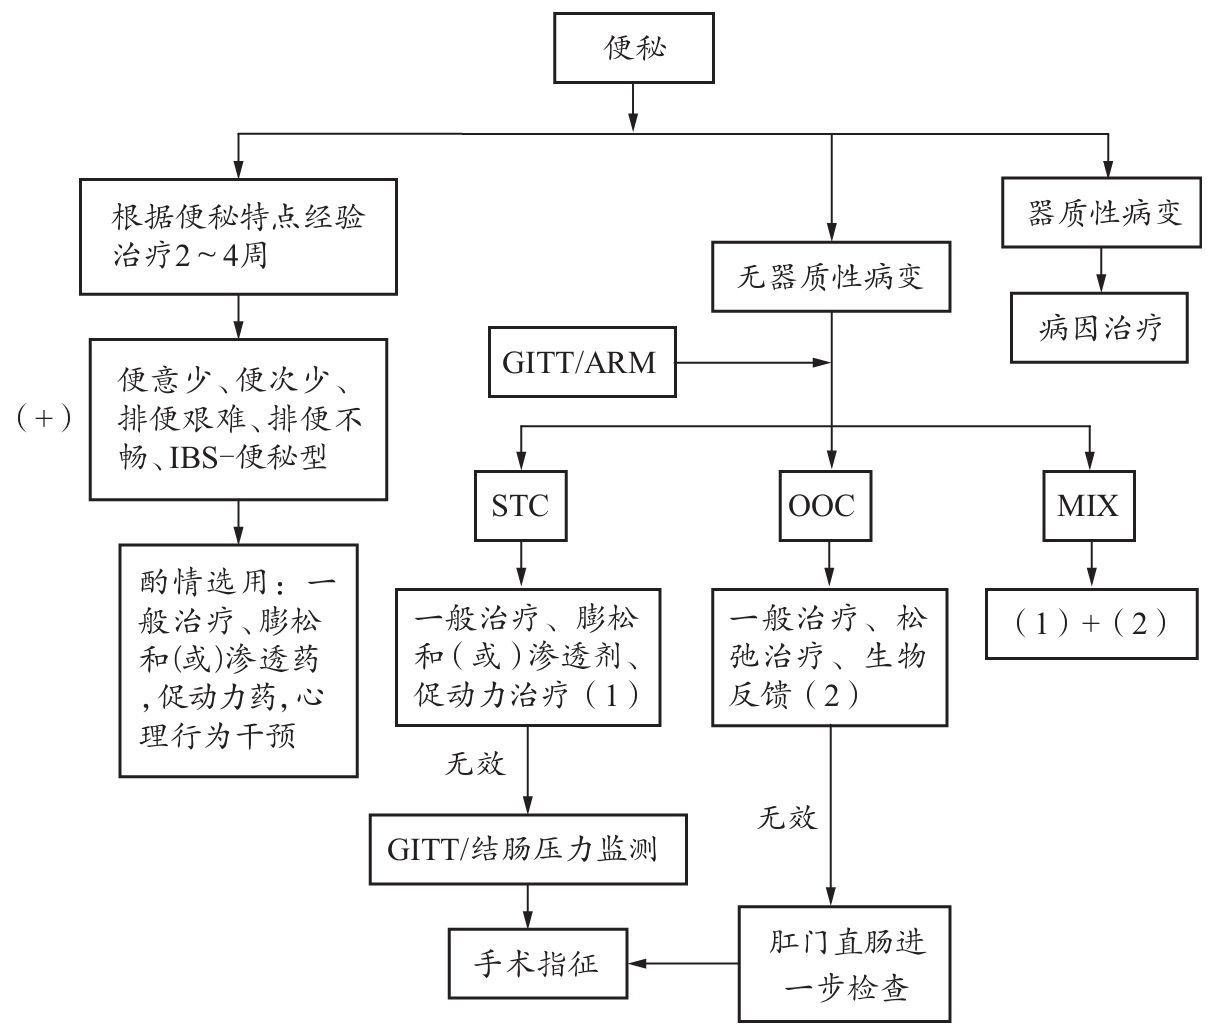
\includegraphics{./images/Image00096.jpg}
 \captionsetup{justification=centering}
 \caption{便秘的治疗程序}
 \label{fig3-8-2}
  \end{figure} 

【治疗方案】 治疗目的是缓解症状,恢复正常肠动力和排便生理功能。因此,总的原则是个体化的综合治疗,包括调整患者的精神心理状态,推荐合理的膳食结构,建立正确的排便习惯;对有明确病因者进行病因治疗;需长期应用通便药维持治疗者,应避免滥用泻剂。外科手术应严格掌握适应证,并对手术疗效作出客观预测。

1.
一般处理 帮助患者充分认识导致便秘的因素,解除患者对排便过度紧张的心理负担。建议增加饮水量和体力活动量,指导患者养成良好的排便习惯。

2. 药物治疗

(1)膳食纤维和膳食纤维制剂:便秘者需要更多的纤维素维持大便的体积和肠道传输功能。增加膳食中的纤维素,必要时通过膳食纤维制剂补充,膳食纤维制剂包括麦麸、甲基纤维素等。应注意大剂量膳食纤维制剂可导致腹胀。可疑肠梗阻者禁用。

(2)通便药:选用通便药时应考虑药效、安全性、药物依赖性以及价效比。避免长期使用刺激性泻剂。对粪便嵌塞者,可用清洁灌肠或用液体石蜡等直肠给药,软化粪便。便秘合并痔者可用复方角菜酸酯制剂。

容积类轻泻剂(膨松剂):通过增加粪便中的水含量和固形物而起到通便作用,如欧车前。

渗透性泻剂:包括不被吸收的糖类、盐类泻剂和聚乙二醇。不被吸收的糖类可增加肠腔内粪便的容积,刺激肠道蠕动,可用于轻、中度便秘的治疗(如乳果糖)。盐类制剂(如硫酸镁)在肠道不完全吸收,使水分渗入肠腔,应注意过量应用可引起电解质紊乱,对老年人和肾功能减退者应慎用。聚乙二醇口服后不被肠道吸收、代谢,能有效治疗便秘,且其含钠量低,不引起肠道净离子的吸收或丢失,不良反应少。

刺激性泻剂:包括酚酞、蒽醌类药物、蓖麻油等,能刺激肠蠕动,增加肠动力,减少吸收。此类泻剂易出现药物依赖、电解质紊乱等不良反应,长期应用可引起结肠黑变病并增加大肠癌的危险性。

(3)促动力剂:增加肠道动力,因而对STC有较好的效果,但某些作用于5-羟色胺(HT)受体的药物有潜在增加心血管疾病的危险。

(4)中药:国内文献报道中药(包括中成药制剂和汤剂)能有效缓解慢性便秘的症状。中药对慢性便秘疗效的评估尚需更多循证医学研究的支持。

3.
生物反馈治疗 适用于功能性排便障碍。通过治疗使患者排便时盆底肌矛盾性收缩得到纠正。部分患者能同时改善直肠感觉功能、直肠推进蠕动与肛门松弛的协调性。

4.
手术治疗 真正需要外科手术治疗的慢性便秘患者尚属少数,当患者症状严重影响工作和生活,且经过一段时间严格的非手术治疗无效时,可考虑手术治疗。要掌握好手术适应证。术前需行结肠气钡对比造影、结肠传输试验、排粪造影、肛门直肠压力测定、球囊逼出试验,必要时行盆底肌电图或盆腔多重造影等特殊检查。手术治疗有一定的复发率。手术后应给予必要的药物治疗。

【疗效观察与随访】

1. 观察指标 排便情况(次数、大便性状)、粪常规检查、腹部B超等。

2. 治愈标准 症状、体征消失,半年内未再发生便秘。

3. 随访 治疗后有无再出现便秘,治疗效果观察。

【治疗经验与解析】

1.
在选用通便药方面,应注意药效、安全性及药物的依赖作用。目前主张选用膨松剂和渗透性通便剂。对慢输型便秘,必要时可加用肠道促动力剂。多种中成药具有通便作用,需注意成药成分,尤其是长期用药可能带来的不良反应。对粪便嵌塞的患者,清洁灌肠或结合短期使用刺激性泻剂解除嵌塞,再选用膨松剂或刺激性药物,保持大便通畅。开塞露和甘油栓有软化粪便和刺激排便的作用。如内痔合并便秘,可用复方角菜酸酯栓剂。

2.
慢性便秘的4种常见表现包括:①便意少,便次也少;②排便艰难、费力;③排便不畅;④便秘伴有腹痛或腹部不适。应仔细辨别,个体化指导治疗。

\section{慢性腹泻}

健康人每日解成形便一次,粪便量不超过200\textasciitilde{}300g。每日排便次数增多\textgreater{}3次,每日粪便量增加\textgreater{}200g,粪质稀薄(含水量\textgreater{}85\%),即为腹泻。病程超过4周,即为慢性腹泻。

腹泻是常见病,但是很多腹泻,尤其是慢性腹泻,并非一定由肠道疾病引起,切不可掉以轻心。经常引起腹泻的其他疾病包括:糖尿病、甲亢、胰腺炎、胰腺癌、胆石症、胆囊切除术后等。

【治疗方案】 腹泻是症状,治疗应针对病因。但相当部分的腹泻需根据其病理生理特点给予对症和支持治疗。

1.
病因治疗 感染性腹泻需根据病原体进行治疗。乳糖不耐受症和麦胶性乳糜泻需分别剔除食物中的乳糖或麦胶类成分。高渗性腹泻应停食高渗的食物或药物。胆盐重吸收障碍引起的结肠腹泻可用考来烯胺吸附胆汁酸而止泻。治疗胆汁酸缺乏所致的脂肪泻,可用中链脂肪代替日常食用的长链脂肪,前者不需经结合胆盐水解和微胶粒形成等过程而直接经门静脉系统吸收。

2.
对症治疗 ①纠正腹泻所引起的失水、电解质紊乱和酸碱平衡失调。②对严重营养不良者,应给予营养支持。谷氨酰胺是体内氨基酸池中含量最多的氨基酸,虽为非必需氨基酸,但它是生长迅速的肠粘膜细胞所特需的氨基酸,与肠粘膜免疫功能、蛋白质合成有关。因此,对弥漫性肠粘膜受损者,谷氨酰胺是粘膜修复的重要营养物质,在补充氨基酸时应注意补充谷氨酰胺。③严重的非感染性腹泻可用止泻药。

【疗效观察与随访】

1.
观察指标 监测患者的一般情况、腹泻次数变化、粪便性状、症状、体征、血常规、粪便常规和隐血试验,粪便培养,肝肾功能等,腹泻与腹痛的变化、缓解与加重的因素以及营养状态。

2. 疗效判定

治愈标准:腹泻停止,大便性状正常,3个月内未复发。

好转标准:腹泻减轻,同时有腹痛。

3.
随访 注意病情观察,避免并发症。定期复查粪常规、隐血试验、粪便培养等。

【治疗经验与解析】

1.
应重视慢性腹泻的并发症 ①腹泻病程较长,常可引起营养不良和各种维生素缺乏症。腹泻与营养不良,往往造成恶性循环,导致不良后果。维生素A缺乏可引起干眼症及角膜软化症,维生素D缺乏可引起低钙血症。②感染:常见有中耳炎、口角炎、上呼吸道感染、支气管炎、肺炎、疖肿、败血症、泌尿道感染及静脉炎等。各种感染可以是腹泻的病因,但也可能起于腹泻之后,因全身抵抗力降低而继发。迁延性腹泻或原有营养不良,常易并发真菌感染,如鹅口疮、真菌性肠炎,甚至引起全身性真菌病。③重型腹泻可能出现黄疸,常见于营养不良及重症败血症患者,预后不良。④其他如急性肾衰竭、弥漫性血管内凝血、感染性休克、中毒性脑病等,如处理不当还可发生急性心力衰竭、高血钾、中毒性肠麻痹、肠出血、肠套叠等,偶可见肠穿孔和腹膜炎。

2.
关于本病抗生素的使用 ①慎用抗菌药物。分离出特异性病原菌的感染,可根据药敏试验选用。②沙门菌肠炎、副溶血弧菌肠炎均有自限性,抗菌药的使用不缩短病程,可延长排菌时间、引起菌群失调并增加耐药菌株,但老人、婴儿、原有严重慢性消耗性疾病(AIDS、DM、脏器功能衰竭)者抗菌药物指征可放宽。

\section{慢性病毒性肝炎}

\subsection{慢性乙型肝炎}

慢性乙型肝炎(CHB)是一种严重危害人类健康的常见病,其防治是一个全球性公共卫生问题。我国乙型肝炎病毒(HBV)HBsAg阳性率9.75\%,约有1.2亿人,占全球的1/3,其中约1/4将发展为慢性肝病,部分患者可发展为肝硬化,甚至演变为肝癌。加强病毒性肝炎的防治,探求CHB的有效防治方法,是当前亟待解决的重大课题。

【治疗程序】 如图\ref{fig3-10-1}所示。

\begin{figure}[!htbp]
 \centering
 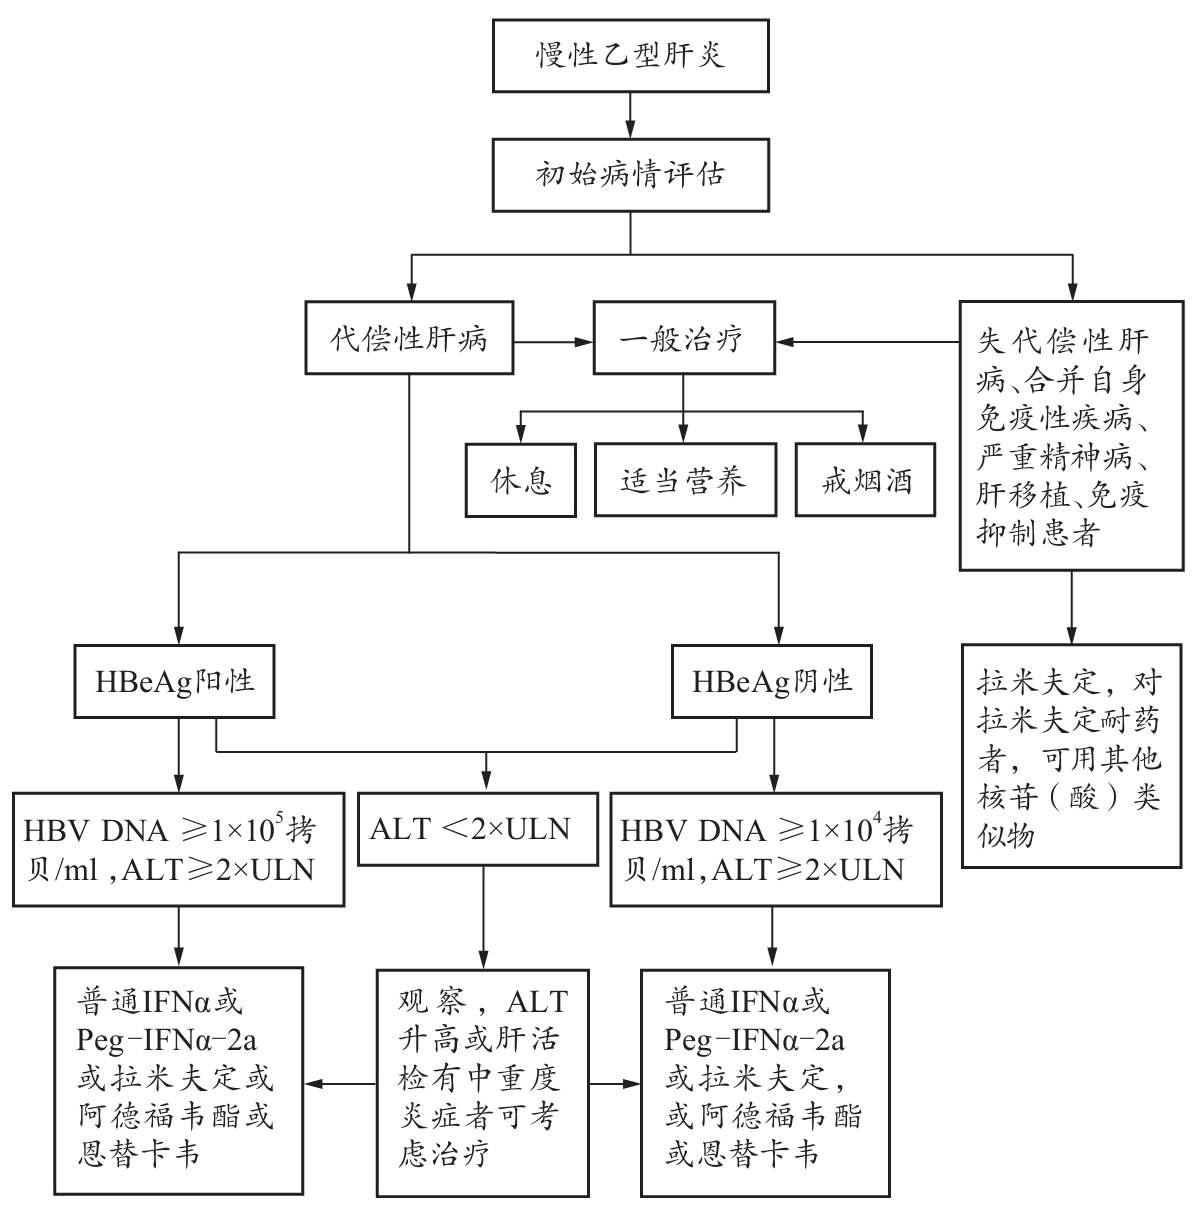
\includegraphics{./images/Image00097.jpg}
 \captionsetup{justification=centering}
 \caption{慢性乙型肝炎的治疗程序}
 \label{fig3-10-1}
  \end{figure} 

【治疗方案】 治疗目标为:①抑制病毒复制,促进病毒清除。②减轻肝脏炎症及坏死,促进肝细胞修复。③缓解、减轻临床症状,阻止或延缓发展为肝硬化。④减少HBV相关性肝癌的发生概率。⑤改善患者的生活质量,延长患者的生存期。

1.
一般治疗 去除和避免肝损因素,适当的营养和充分的休息,给予免疫调节治疗、基因治疗、“保肝”药物治疗、心理治疗及基础治疗以及中医中药等治疗。

2. 抗病毒治疗

(1)抗病毒治疗的药物:目前,已有核苷类似物(NUCs)及干扰素(IFN)α两大类药物用于CHB治疗。

NUCs可分为三类:L核苷类(拉米夫定、替比夫定和恩曲他滨)、脱氧鸟苷类似物(恩替卡韦)以及无环核苷磷酸盐化合物(阿德福韦酯和替诺福韦酯)。我国已批准拉米夫定、阿德福韦酯、恩替卡韦及替比夫定用于CHB治疗。

干扰素可分为普通IFN及Peg-IFN,我国均已批准用于CHB的治疗。Peg-IFN与NUCs治疗CHB的优缺点见表\ref{tab3-10-1}。

\begin{table}[htbp]
    \centering
    \caption{Peg-IFN与NUCs治疗慢性乙型肝炎的优缺点}
    \label{tab3-10-1}
    \begin{tabular}{lll}
\toprule
& 优点 & 缺点\tabularnewline
\midrule
Peg-IFN &
\vtop{\hbox{\strut 有限疗程}\hbox{\strut 无耐药发生}\hbox{\strut HBeAg或HBsAg血清学转换率高}}
&
\vtop{\hbox{\strut 抗病毒疗效一般}\hbox{\strut 患者耐受性好}\hbox{\strut 皮下注射}}\tabularnewline
NUCs &
\vtop{\hbox{\strut 抗病毒作用强}\hbox{\strut 耐受性好}\hbox{\strut 口服给药}}
&
\vtop{\hbox{\strut 未达满意的治疗终点者疗程不固定}\hbox{\strut 耐药变异率高}\hbox{\strut HBeAg或HBsAg血清学转换率低}}\tabularnewline
\bottomrule
    \end{tabular}
\end{table}

目前,有循证医学证据支持的CHB治疗策略仍为应用IFN-α或NUCs的单药治疗。

(2)干扰素治疗慢性乙型肝炎:

干扰素-α(普通或Peg-IFN)的主要优点:即不存在耐药,有免疫介导的抗HBV作用,从而使治疗结束时HBVDNA低于检测下限的患者有机会得到持久病毒学应答以及HBsAg消失。因此,考虑到CHB抗病毒治疗的长期性和为避免长期治疗中耐药的发生风险,推荐Peg-IFNα作为优先选择的药物之一。

干扰素治疗的适应证与禁忌证:对于HBeAg阳性或HBeAg阴性的CHB患者,干扰素治疗的适应证主要考虑三个方面:血清HBVDNA水平、血清转氨酶水平、组织学分级与分期。患者的HBVDNA水平超过1×10$^{4}$
拷贝/ml(1
IU/ml≈5.26拷贝/ml)和(或)血清ALT水平超过正常上限(ULN),肝活检显示中重度活动性炎症、坏死和(或)纤维化时,应考虑治疗。

治疗适应证还应考虑患者年龄、健康状况以及抗病毒药物的可获得性,并应考虑下列特殊人群:①免疫耐受期患者:对于大多数30岁以下、ALT持续正常、HBVDNA水平较高(\textgreater{}10$^{8}$
拷贝/ml)、无任何肝脏疾病征象、无肝癌或肝硬化家族史的患者,不要求即刻行肝活检或治疗,但必须进行随访。②轻度CHB患者:对于ALT轻度升高(\textless{}2×ULN)、组织学检查示轻度病变的患者,可以不治疗,但必须随访。③代偿期肝硬化患者:如果检测到HBVDNA,即使ALT水平正常和(或)HBVDNA\textless{}10$^{4}$
拷贝/ml,也应考虑治疗。④乙型肝炎相关的失代偿期肝硬化患者、自身免疫性疾病以及未控制的严重抑郁或精神病患者是应用IFN-α的禁忌证。

药物及剂量和疗程选择:普通干扰素-α:HBeAg阳性的CHB患者,普通IFN-α的成人推荐剂量为5MIU(可根据患者耐受情况适当调整剂量),儿童6MIU/m{2}
体表面积(每周3次,最大5MIU),隔日1次,皮下注射,一般疗程为48周。如有应答,为提高疗效亦可延长疗程至更长。而HBeAg阴性的CHB患者,普通IFN-α的疗程至少为48周,一项研究建议24个月疗程可能会提高持久应答率。

聚乙二醇化干扰素-α:目前的Peg-IFNα-2a成人推荐治疗剂量180μg,每周1次,皮下注射,疗程48周;Peg-IFNα-2b成人推荐治疗剂量为115μg/kg,每周1次,皮下注射,疗程48周。剂量应根据患者耐受性等因素决定。

干扰素治疗应答的定义:①原发无应答:治疗24周HBVDNA从基线水平下降小于1log10IU/ml。②病毒学应答:治疗24周HBVDNA水平降低至小于4log10IU/ml。③血清学应答:HBeAg阳性的CHB患者出现HBeAg血清学转换。

应答预测:由于患者感染途径、性别、年龄、遗传背景、病程长短、肝脏病变程度、治疗药物敏感度、药物不良反应及耐受力、病毒基因型等诸多因素不同,患者的免疫清除功能也不相同,按同样方案治疗后是否出现应答和出现应答的时间也不尽一致。预测发生HBeAg血清学转换的治疗前因素是低病毒载量(HBVDNA\textless{}10拷贝/ml)、高血清ALT水平(\textgreater{}3×ULN)、肝活检示炎症活动较明显。治疗12周时HBVDNA降至\textless{}10$^{5}$
拷贝/ml。HBeAg阳性患者发生HBeAg血清学转换的概率为50\%;HBeAg阴性患者获得持续病毒学应答的概率为50\%。治疗24周时HBeAg水平下降可以预测HBeAg血清学转换。

HBsAg定量在预测获得持续病毒学应答和HBsAg消失的作用有待进一步研究证实。HBV基因A型、B型患者较C型和D型患者对IFN-α的应答更好。但基因型对个体的预测价值较差,不能单独作为治疗选择的依据。

(3)核苷(酸)类似物治疗慢性乙型肝炎:

核苷(酸)类似物治疗慢性乙型肝炎的适应证:HBeAg阳性/HBeAg阴性的CHB患者及肝硬化(包括代偿期及失代偿期)患者均可应用NUCs进行初始治疗。与IFN-α类似,对于HBeAg阳性的CHB患者,HBeAg血清学转换是最常用的疗效评价指标。较高的基线ALT水平(\textgreater{}3×ULN)和较低的基线HBVDNA(\textless{}10$^{7}$
拷贝/ml)是应用NUCs治疗时HBeAg血清学转换的预测因素。

药物选择及疗程:虽然各种NUCs均可作为一线治疗药物,但应尽量选择那些抗病毒作用强且耐药变异发生率较低的药物,如替诺福韦酯或恩替卡韦(A1),以减少治疗失败。患者的经济状况和治疗费用也是我国现阶段不容忽视的一个现实问题,选择符合患者经济能力的药物是长期治疗得以持续的前提。①有限疗程治疗:HBeAg阳性CHB患者获得HBeAg血清学转换后可进行NUCs的有限疗程治疗,但不能预测治疗前的具体疗程,因为这取决于HBeAg血清学转换。基线高水平ALT(\textgreater{}3×ULN)、基线HBVDNA\textless{}10$^{7}$
拷贝/ml患者中,HBeAg血清学转换较为常见。一旦获得HBeAg血清学转换,NUCs治疗应继续进行(6\textasciitilde{}12)个月,可使80\%患者获得持久应答(治疗结束后抗HBe持续阳性)。②长疗程治疗:适用于那些停止治疗后不能获得持久病毒学应答并需进一步治疗的患者,即不能获得HBeAg血清学转换的HBeAg阳性和HBeAg阴性患者。肝硬化患者也适用,不论其HBeAg状态或治疗中HBeAg发生血清学转换。单药治疗应该选用那些抗病毒作用强、耐药率相对较低的药物,如替诺福韦酯或恩替卡韦。无论用药与否,保持HBVDNA低于检测线是基本的疗效指标。恩替卡韦和替诺福韦酯的远期(如5\textasciitilde{}10年后)疗效、安全性和耐受性尚不清楚。对于NUCs来说,长期治疗的主要关注点是选择性耐药位点的出现。这与治疗前血清HBVDNA水平、病毒抑制速度、疗程及是否曾使用NUCs治疗有关。基因型耐药的发生与耐药突变检测方法的敏感性及所检测的人群有关。

应答的定义:①原发无应答:治疗12周(有些NUCs为24周)时,HBVDNA从基线水平下降\textless{}1log10IU/ml。②病毒学应答:治疗48周时,HBVDNA下降到实时PCR法检测线以下。③部分病毒学应答:HBVDNA下降\textgreater{}1log10IU/ml,但仍高于实时PCR法检测下限。拉米夫定和替比夫定的部分病毒学应答评估时间是24周,恩替卡韦、替诺福韦酯和阿德福韦酯应该在48周进行评估。④病毒学突破及耐药:治疗过程中HBVDNA从最低水平升高\textgreater{}1log10IU/ml。常伴有以ALT水平升高为特征的生物化学突破。NUCs治疗过程中病毒学突破的主要原因是患者依从性差或针对NUCs的HBV耐药变异。

【疗效观察与随访】

1.
观察指标 患者详细的病史及家族史、症状、体征及定期体格检查。血清ALT、AST、胆红素、凝血酶原时间、胆碱酯酶、血清白蛋白和甲胎蛋白。HBsAg、抗-HBs、HBeAg、抗-HBe、HBVDNA,为除外重叠感染,还应检测抗-HCV、抗-HDV和抗-HIV。必要时可对肝脏、胆囊和脾脏进行超声、CT或MRI检查。对达到CHB诊断标准的患者进行肝脏组织病理检查,确定炎症、坏死和纤维化程度。

2.
好转标准 症状、体征显著改善,相关检测项目接近正常,病情稳定在半年以上。

3. 随访

(1)注意病情观察:观察症状、体征等变化,避免肝损因素,避免合并症、并发症。

(2)接受IFN-α治疗的患者:应每月监测全血细胞计数和血清ALT水平。12周和24周时评估血清HBVDNA水平以验证初始应答。

HBeAg阳性患者:需监测治疗12周、24周、48周和治疗后24周时HBeAg和HBeAb。HBeAg发生血清学转换且血清ALT正常、实时PCR法检测不到血清HBVDNA是较为理想的转归。如发生HBeAg血清学转换,须接受长期随访,因为有发生HBeAg血清学转换逆转或转为HBeAg阴性CHB的可能。如果HBVDNA检测不到,在发生HBeAg血清学转换后6个月需监测HBsAg,此时该人群HBsAg消失的概率增加。一旦出现原发无应答,应考虑调整治疗方案:停止干扰素治疗,换用核苷(酸)类似物。

HBeAg阴性患者:48周治疗期间同样需监测药物的安全性和有效性。出现病毒学应答(HBVDNA\textless{}10拷贝/ml)与肝病缓解相关。实时PCR法检测不到HBVDNA是较为理想的,因为持续应答与HBsAg消失有关。如果检测不到HBVDNA,6个月后应检测HBsAg。对于所有IFN-α治疗的患者,都应监测干扰素相关不良反应。

(3)接受NUCs治疗的患者:治疗期间应至少每3个月检测1次ALT、HBeAg和(或)HBVDNA;如用阿德福韦酯,还应监测患者肾功能(血肌酐、尿素氮);如应用替比夫定,尚须监测肌酸激酶(CK)。HBeAg和HBsAg定量检测的临床意义及价值有待进一步探讨。

【治疗经验与解析】

1.
IFN-α的普遍应用和某些不合适的应用,导致部分不良反应,其中大部分为轻度或自限性,极少数为严重不良反应,应引起重视。

(1)流感样症状:为IFN-α应用早期最常见的不良反应,表现为发热、寒战、头痛、乏力、全身不适、心动过速及肌肉关节酸痛。大部分患者可以耐受,在注射数针后会逐渐减轻、消失。可在干扰素注射初期同时口服阿司匹林、对乙酰氨基酚或其他非甾体类解热镇痛药以减轻症状。极个别患者由于高热、全身关节疼痛等持续而严重的流感样症状而中止治疗。

(2)血液系统表现:IFN-α有不同程度的骨髓抑制,部分患者可发生白细胞总数、中性粒细胞和血小板计数的轻中度下降。若在治疗前计数正常,可继续IFN治疗,同时应用刺激白细胞生长的药物。中性粒细胞明显降低者,可试用粒细胞集落刺激因子(G-CSF)或粒细胞巨噬细胞集落刺激因子(GM-CSF)治疗。外周血白细胞总数≤1.5×10$^{9}$
/L或中性粒细胞计数≤0.75×10$^{9}$ /L或血小板计数≤50×10$^{9}$
/L的患者,应下调IFN剂量继续治疗并加强监测。外周血白细胞总数≤1.0×10$^{9}$
/L或中性粒细胞计数≤0.5×10$^{9}$ /L或血小板计数≤30×10$^{9}$
/L的患者,应暂停使用,定期随诊观察,好转后再从小剂量开始治疗。

(3)精神和神经系统表现:包括乏力、衰弱、嗜睡、缺少主动性、易怒、思维混乱、冷漠、情绪及认知改变等,发生机理尚不明确。

(4)免疫和内分泌系统表现:IFN具有免疫调节作用。在治疗中可出现抗甲状腺球蛋白及抗微粒体抗体等甲状腺抗体。其他的自身免疫性和内分泌系统疾病也会发生,但以甲状腺疾病最重要,甲状腺功能减退最常见,应定期监测甲状腺功能。

(5)其他不良反应:少数患者可出现心律不齐、心脏缺血性疾病和心肌病,对40岁以上和既往有心脏病的患者,IFN治疗期间需加强心脏监护。少数IFN治疗的患者可出现不同程度的肾毒性的表现,包括轻度蛋白尿、尿白细胞增多、镜下血尿和轻度肾功能减退,血肌酐及尿素氮升高等,大多停用IFN后可自行恢复。在IFN治疗的早、中期,血清转氨酶可有轻中度升高,随着疗程继续而恢复正常。部分患者可出现胃肠方面的不良反应,如恶心、呕吐、消化不良、腹泻、腹痛等症状。轻微脱发也相对常见,但可以恢复。罕见的其他不良反应还包括视网膜病变甚至视力障碍、间质性肺炎、听力障碍甚至突发性耳聋等。

2.
NUCs经肾代谢,推荐对肌酐清除率降低的患者应调整剂量。肝脏不同程度损伤的患者药物浓度相当,但未进行充分研究。肝硬化患者出现耐药后若不及时挽救治疗,病情可能恶化,需要加强监测(前3个月每月1次)。患者发生并发症时须紧急处理。服用肾毒性药物的患者和服用替诺福韦酯或阿德福韦酯10mg/d的患者,应适当监测肾毒性并调整药物剂量。曾有阿德福韦酯在较大剂量(50mg/d)时肾脏损害的报道,故合并肾脏疾病者应慎用;替比夫定可导致肌肉损害(表现为肌酸激酶升高,严重者伴肌肉酸痛甚至横纹肌溶解),故合并肌炎者应避免使用该药。

曾有HIV阳性患者服用替诺福韦酯发生骨矿物质密度下降的报道,但须进行长期研究。恩替卡韦致癌作用的长期研究正在进行。已有替比夫定治疗CHB发生肌病的报告。在接受Peg-IFN联合替比夫定治疗的患者中,可发生周围神经病变,应避免这两种药物联合应用。

3.
大多数接受NUCs治疗的CHB患者难以通过短期治疗实现持久应答,需接受长期治疗,这必将增加病毒耐药的风险,随着NUCs种类的增加,HBV耐药变异的复杂性也大大增加。目前耐药变异的概念包括3方面内容:耐药预防、耐药预测和挽救治疗(rescue
therapy)。

(1)耐药预防:选择强效、低耐药的药物,即所谓高耐药基因屏障和(或)低耐药发生率药物(如恩替卡韦或替诺福韦酯)单药治疗是已得到公认的耐药预防方案。另一预防或延迟耐药发生的方法为联合治疗策略,抗病毒治疗起始即联合两种以上药物同时使用;该方案尚无符合循证医学原则的临床数据支持,并且何种药物联用方能实现最优效价比尚待进一步明确。

(2)耐药预测:多种因素可能与HBV对NUCs耐药发生率相关,包括应用NUCs的种类、初始治疗时HBVDNA载量及ALT水平、有肝纤维化/肝硬化基础、曾接受过NUCs抗病毒治疗等。此外,越来越多的研究提示早期病毒学应答情况是预测耐药发生率的重要指标,从而提出治疗路线图的概念。

(3)挽救治疗:绝大多数NUCs耐药者,尤其是失代偿期肝硬化患者,需及早进行挽救治疗。通常病毒学突破先于生物化学突破,在生物化学突破前进行挽救治疗可使患者免于发生肝炎突发、肝病恶化。

4. 关于联合治疗

(1)干扰素与NUCs联合治疗:联合治疗的潜在优势是附加的或者共同的抗病毒效应以及减少或延迟耐药的发生。缺点是花费增加、毒性提高及药物间相互作用。目前仍无资料支持联合治疗可降低那些单独应用时有低耐药风险的抗病毒化合物的耐药发生几率。

(2)不同种类NUCs联合治疗:尚未见反映初始接受恩替卡韦和替诺福韦酯治疗的患者接受NUCs联合治疗优势的资料,相关的治疗试验正在进行中。对那些出现耐药可能性高的患者(基线HBVDNA水平高)或因存在基础疾病(肝硬化)而一旦耐药将可能危及生命的患者,有专家推荐联合治疗以防止潜在耐药的发生。然而NUCs联合,尤其是与恩替卡韦或替诺福韦酯联合治疗的长期安全性尚不明确,而且这种联合法花费也较高。可考虑替诺福韦酯加拉米夫定或替诺福韦酯加恩曲他滨复合片剂用于该类患者的治疗。

5.
关于治疗终点 CHB患者的抗病毒治疗必须将HBVDNA降至尽可能低的水平。抑制病毒复制一方面可使生物化学指标恢复、组织学改善、预防并发症的发生;另一方面还能降低核苷(酸)类似物(NUCs)的耐药风险,增加HBeAg阳性CHB患者的HBeAg血清学转换率以及HBeAg阳性/HBeAg阴性的CHB患者HBsAg低于检测下限的可能性。

(1)理想的治疗终点:无论HBeAg阳性还是HBeAg阴性的CHB患者,理想的治疗终点是HBsAg低于检测下限,伴或不伴抗HBs高于检测下限。达到理想终点往往预示炎症缓解、远期预后改善。

(2)满意的治疗终点:对于HBeAg阳性的CHB患者,满意的治疗终点是持续的HBeAg血清学转换,这种转换多伴随预后的改善。

(3)可获益的治疗终点:对于未能达到HBeAg血清学转换的HBeAg阳性/HBeAg阴性患者,在NUCs持续治疗或干扰素(IFN)α治疗后维持HBVDNA低于检测下限,患者仍然可以获益,使疾病进展缓慢。

\subsection{慢性丙型肝炎}

丙型肝炎是一种主要经血液传播的疾病,丙型肝炎病毒(HCV)感染超过6个月,或发病日期不明、无肝炎史,但肝脏组织病理学检查符合慢性丙型肝炎,或根据症状、体征、实验室及影像学检查结果综合分析,即可诊断慢性丙型肝炎(chronic
hepatitis
C,CHC)。HCV慢性感染可导致肝脏慢性炎症坏死和纤维化,部分可发展为肝硬化甚至肝细胞癌(HCC)。

【治疗程序】

1. CHC基因1型及4\textasciitilde{}6型感染患者处理与治疗程序(图\ref{fig3-10-2})。

\begin{figure}[!htbp]
 \centering
 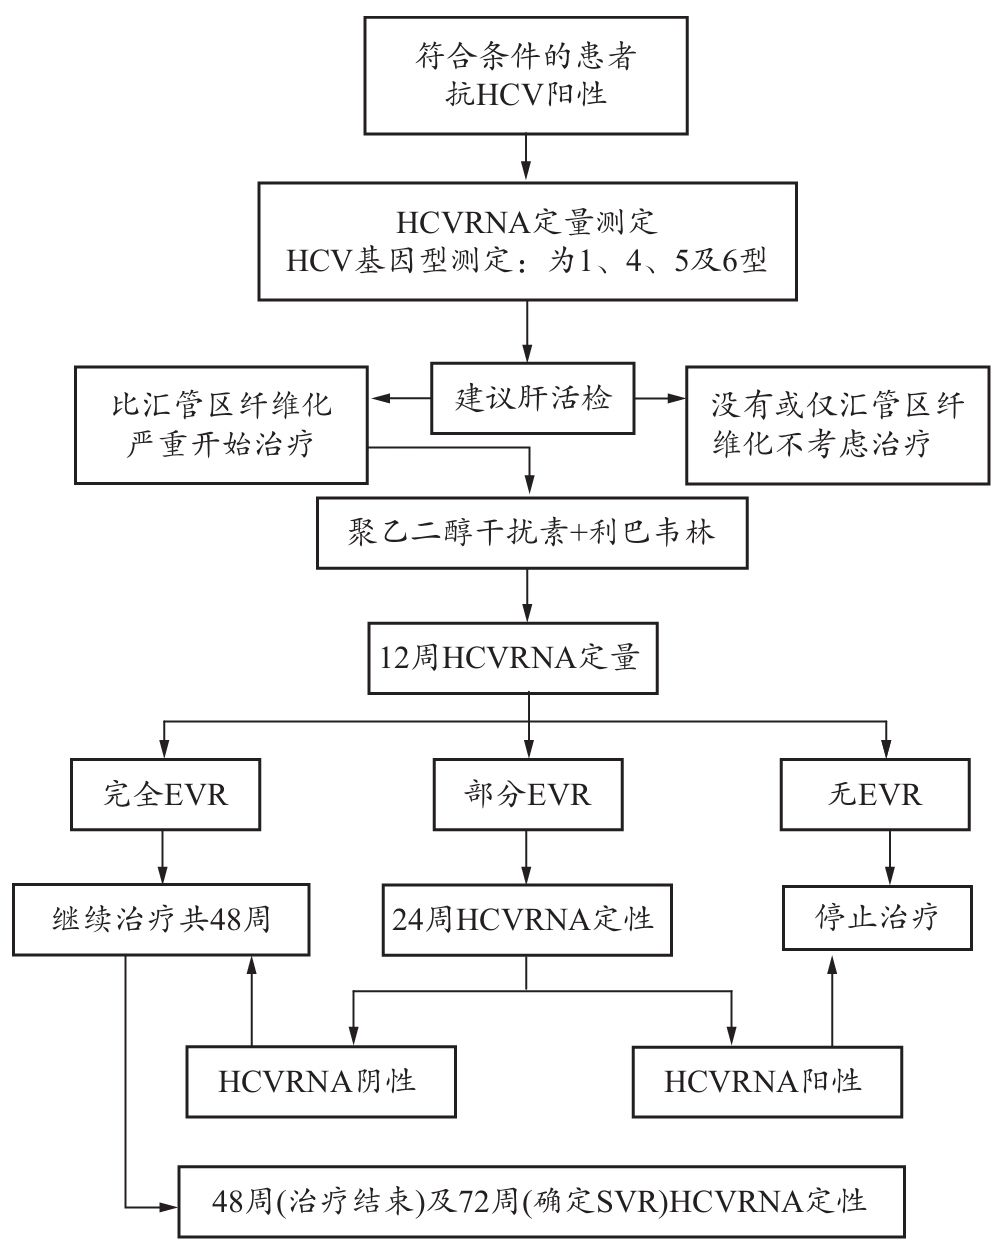
\includegraphics{./images/Image00098.jpg}
 \captionsetup{justification=centering}
 \caption{CHC基因1型及4\textasciitilde{}6型感染患者处理与治疗程序}
 \label{fig3-10-2}
  \end{figure} 

2. CHC基因2或3型感染患者处理与治疗程序(图\ref{fig3-10-3})。

\begin{figure}[!htbp]
 \centering
 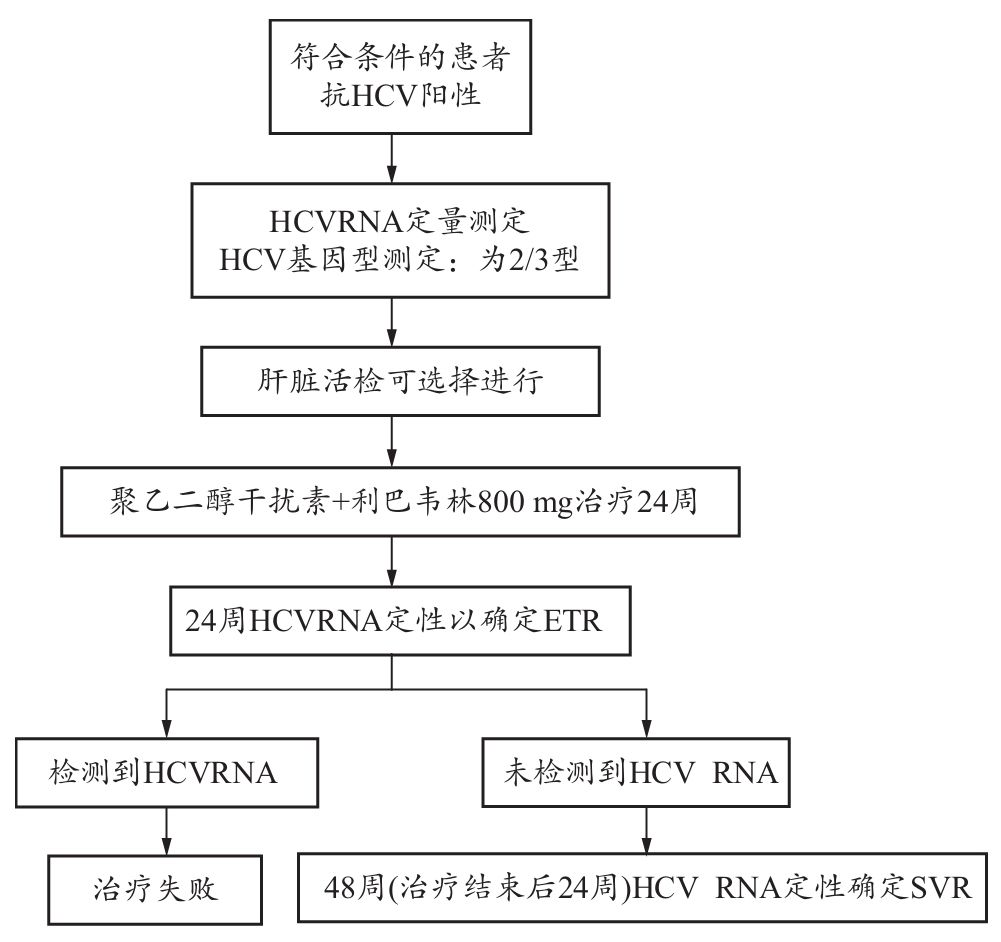
\includegraphics{./images/Image00099.jpg}
 \captionsetup{justification=centering}
 \caption{慢性HCV基因2或3型感染患者处理与治疗程序}
 \label{fig3-10-3}
  \end{figure} 

【治疗方案】

1.
一般治疗 适当休息,合理饮食,避免饮酒,心理辅导支持,增加患者治疗的依从性。

2. 药物及相关治疗

(1)改善和恢复肝功能:①非特异护肝药:维生素类、还原性谷胱甘肽、肝泰乐等。②降酶药:苦参碱、联苯双酯、甘草提取物、垂盆草类等,此类药物显效后须逐渐减量,避免ALT反跳。③退黄药物:丹参、茵栀黄、门冬氨酸钾镁、腺苷蛋氨酸、苯巴比妥类、皮质激素类、低分子右旋糖酐,应用糖皮质激素须慎重,无禁忌证时选用。

(2)免疫调节:胸腺肽或胸腺素、转移因子、特异性免疫核糖核酸等,某些中草药如香菇多糖、猪苓多糖等亦有免疫调节作用,可以使用。

(3)抗肝纤维化:主要有丹参、冬虫夏草、核仁提取物、干扰素等。

3. 抗病毒治疗

(1)抗病毒治疗目标与抗病毒治疗应答的类型:抗病毒治疗的长期目标为降低HCV相关肝硬化、肝衰竭与肝细胞癌的发生率,降低HCV相关病死率,改善患者生活质量。HCV感染一般病情缓慢进展,抗病毒疗效评价多采用短期的临床指标,包括病毒学应答、生化学应答与肝组织学应答等指标。其中病毒学应答指标中的持续病毒学应答(SVR)是当前评判疗效的最主要指标。抗病毒治疗应答的类型,参见下表(表\ref{tab3-10-2})\footnote{快速病毒学应答(RVR);检测下限(LLD);完全早期病毒学应答(cEVR);部分早期病毒学应答(pEVR);治疗结束时病毒学应答(ETVR)。}。

\begin{table}[htbp]
    \centering
    \caption{CHC抗病毒治疗病毒学应答类型}
    \label{tab3-10-2}
    \begin{tabular}{ll}
\toprule
病毒学应答指标 & 定义\tabularnewline
\midrule
快速病毒学应答 & 治疗4周,HCVRNA载量低于检测下限(LLD)\tabularnewline
完全早期病毒学应答 & 治疗12周,HCVRNA载量低于LLD\tabularnewline
部分早期病毒学应答 &
治疗12周,HCVRNA下降\textgreater{}2log10IU/ml,但未低于LLD\tabularnewline
治疗结束时病毒学应答 & 治疗结束时HCVRNA载量低于LLD\tabularnewline
持续病毒学应答 & 达到ETVR,停药随访24周仍维持HCV
RNA载量低于LLD\tabularnewline
复发 & 达到ETVR,但停药后HCVRNA又可被检出\tabularnewline
突破 & 治疗期间曾出现HCVRNA低于LLD,但继续治疗HCV
RNA又可检出\tabularnewline
无应答 & 治疗24周,HCVRNA仍可被检出。\tabularnewline
\bottomrule
    \end{tabular}
\end{table}


(2)抗病毒治疗药物与方案:聚乙二醇化干扰素(Peg-IFN)联合利巴韦林(RBV)是目前慢性丙型肝炎抗病毒治疗的标准方案,约65\%患者可取得持续病毒学应答(SVR)。近年来,应答指导治疗(RGT)、特殊患者的治疗以及抗病毒治疗不良反应的处理均取得迅速进展。在条件允许的情况下,应推荐患者采用Peg-IFN联合RBV的方案治疗,尤其是对于基因1型和(或)高基线HCV
RNA载量(HCV RNA\textgreater{}6×10$^{5}$
IU/ml)的患者。药物与方案参见下表(表\ref{tab3-10-3}及表\ref{tab3-10-4})。

\begin{table}[htbp]
    \centering
    \caption{基因2型与3型治疗方案}
    \label{tab3-10-3}
    \begin{tabular}{lll}
\toprule
IFN种类与用法 & RBV用法 & 疗程\tabularnewline
\midrule
\vtop{\hbox{\strut Peg-IFNα-2a
180μg,每周1次,皮下注射}\hbox{\strut 或Peg-IFNα-2b
1.5μg/kg,每周1次,皮下注射}\hbox{\strut 或普通IFN
3\textasciitilde{}5MU隔日1次,皮下注射}} & 联合RBV 800mg/d &
24周\tabularnewline
\bottomrule
    \end{tabular}
\end{table}

\begin{table}[htbp]
    \centering
    \caption{基因1型及4\textasciitilde{}6型治疗方案}
    \label{tab3-10-4}
    \begin{tabular}{lll}
\toprule
IFN种类与用法 & RBV用法 & 疗程\tabularnewline
\midrule
Peg-IFNα-2a 180μg,每周1次,皮下注射&\multirow{3}{5cm}{联合RBV 1000mg/d(体重\textless{}75kg)或1200mg/d(体重\textgreater{}75kg)或10.6\textasciitilde{}13mg/(kg·d)}& 48周\tabularnewline\\
Peg-IFNα-2b 1.5μg/kg,每周1次,皮下注射&~&\\
普通IFN3\textasciitilde{}5MU隔日1次,皮下注射&~&\\
\bottomrule
    \end{tabular}
\end{table}

(3)CHC抗病毒治疗的适应证和禁忌证:HCVRNA阳性,无治疗禁忌证的CHC患者均应考虑抗病毒治疗。CHC患者抗病毒治疗的相对与绝对禁忌证见表\ref{tab3-10-5}。

\begin{table}[htbp]
    \centering
    \caption{CHC抗病毒治疗的禁忌证}
    \label{tab3-10-5}
    \begin{tabular}{ll}
\toprule
绝对禁忌证 & 相对禁忌证\tabularnewline
\midrule
肝功能Child-Pugh分级C级 & 肝功能Child-Pugh分级B级\tabularnewline
妊娠 & 甲状腺疾病\tabularnewline
未控制的抑郁性精神疾病 & 接受器官移植\tabularnewline
并存严重的躯体疾病 & 现已控制的精神疾病\tabularnewline
未控制的自身免疫性疾病 &\tabularnewline
对抗病毒治疗药物过敏 &\tabularnewline
患者粒细胞计数、血小板计数与血色素水平不能耐受 &\tabularnewline
\bottomrule
    \end{tabular}
\end{table}

(4)CHC抗病毒治疗的疗效预测因素与方案调整:影响抗病毒疗效的基线指标很多,其中患者基因型与基线HCVRNA载量,是目前最重要的两个预测指标。其他指标还包括性别、年龄、体重、有无胰岛素抵抗以及肝脂肪病变与纤维化程度、是否酗酒以及是否使用静脉毒品等。

这些预测指标有助于临床医生与患者对于可能的治疗结局有充分的认知;也可作为个体化治疗方案的依据。如对于基因1型、高HCVRNA载量和(或)高体重的患者,应更加倾向于推荐Peg-IFN联合RBV治疗;在专业医生指导下,与患者充分沟通,根据患者治疗病毒应答与耐受情况在标准疗程的基础上适当延长患者疗程、调整RBV和(或)IFN的剂量。根据患者治疗过程中病毒学应答情况来预测患者的疗效并相应调整治疗方案,即所谓的应答指导治疗,成为抗病毒治疗的研究热点。目前对SVR预测价值最高的病毒学应答预测指标为RVR和EVR(包括cEVR与pEVR)。IFN抗HCV治疗的前4周可分为两个时相,治疗的24\textasciitilde{}48小时为快速时相,此阶段IFN阻断病毒产生和释放,并清除血液中病毒,并且疗效呈剂量依赖性;第3\textasciitilde{}28日为第二时相,此阶段由IFN促进机体免疫发挥作用,清除病毒感染细胞。因此,治疗4周,HCV
RNA低于检测下限在一定程度上可反映机体具有较强的清除HCV感染能力,这也奠定了以RVR预测患者最终SVR的理论基础。同时这也提示在患者初始治疗时应尽可能采用足量的IFN联合RBV进行治疗。

临床研究证实,RVR对于患者SVR具有强预测作用,且其预测意义不受患者HCV基因型影响。在获得RVR的患者中,有89\%基因1型患者、70\%\textasciitilde{}95\%基因2/3型患者与86\%基因4型患者达到SVR。除非患者不能耐受标准疗程的治疗,应慎重对待缩短RVR患者疗程的做法。EVR对于SVR具有较高阴性预测值。对于未达到cEVR但在治疗24周前实现HCV
RNA低于检测下限的患者,此类患者延长24周疗程可显著提高SVR率。因此,治疗12周与24周期间实现HCV
RNA低于检测下限的基因1与4型患者,可考虑延长疗程至72周;而基因2与3型患者可延长疗程至48周。

4.
CHC 肝内并发症:肝硬化、肝细胞癌、脂肪肝等;肝外并发症:胆管炎、胰腺炎、糖尿病、肾小球肾炎、心肌炎等,其中严重并发症有肝性脑病、上消化道出血、肝肾综合征、自发性腹膜炎等。

【疗效观察与随访】

1.
观察指标 基线检测指标:患者在开始抗病毒治疗前,应对患者进行系统评估,评估指标包括HCV
RNA载量、肝功能、血常规、尿常规、肾功能、自身免疫性指标、甲状腺功能、血糖与血压等;另外应对患者精神状态进行评估。

2.
好转标准 症状改善、各项检测指标接近正常,半年内病情稳定,未见恶化的改变。

3. 随访

(1)HCV
RNA:患者在抗病毒治疗开始后,应在第4周结束时评估RVR,第12周结束时评估EVR,此后每隔12周监测1次HCV
RNA,直至治疗结束。治疗结束后应每12\textasciitilde{}24周检测HCVRNA。

(2)肝功能:治疗过程中应每隔8\textasciitilde{}12周监测1次肝功能指标,停药后应每隔12\textasciitilde{}24周检测肝功能。

(3)血常规:在抗病毒治疗第1个月应每周监测1次血常规,此后应每个月检查1次至6个月,然后每3个月检查1次至治疗结束。

(4)其他指标的监测:应在治疗中每12\textasciitilde{}24周监测甲状腺功能与自身抗体。

(5)精神状态的评估:患者每次随访均应评估精神状态。不同患者对抗病毒治疗反应不同,上述指标的监测间期,尤其是血常规与肝功能等,应根据患者个体情况适当调整。

【治疗经验与解析】

1.
HCV病毒载量的高低与疾病的严重程度和疾病的进展并无绝对相关性,但可作为抗病毒疗效评估的观察指标。在HCVRNA检测中,应注意可能存在假阳性和假阴性结果。

2. HCV
RNA基因分型结果有助于判定治疗的难易程度及制定抗病毒治疗的个体化方案。

3.
病理组织学检查对丙型肝炎的诊断、衡量炎症和纤维化程度、评估药物疗效以及预后判断等方面至关重要。肝组织炎症程度的分级、纤维化程度的分期诊断可参照《病毒性肝炎防治方案》中病理学诊断标准。对于科研或评估治疗药物的疗效,可根据不同需求,选用国内外各种半定量计分方法。

4.
HCV抗病毒治疗无应答或复发患者,确定再治疗方案前应首先充分了解既往抗病毒治疗情况,分析导致无应答或复发的可能原因,包括所应用药物的类型、药物剂量以及减量情况、给药途径、疗程及治疗期间的病毒应答情况;同时要了解患者的治疗依从情况;患者是否酗酒和静脉吸毒等。初次单用IFNα治疗后复发或无应答的患者,可采用Peg-IFN或普通IFNα联合RBV的参考方案再次治疗;初次应用普通IFN联合RBV无应答或复发的患者,可使用Peg-IFN联合RBV的参考方案进行治疗。采用Peg-IFN联合RBV的标准方案治疗无应答的患者再次应用相同方案治疗,仅有\textless{}5\%的患者可获得SVR,且对于此类患者尚无统一意见表明更换IFN种类有效;Peg-IFN联合RBV的标准方案治疗后复发的患者,再治疗的疗效优于无应答患者,但尚无充分证据表明重复以前治疗方案可显著改善患者SVR率。因此,此类患者应当在更换治疗方案后按照病毒学应答情况进行个体化治疗。

5. 特殊患者的治疗

(1)丙型肝炎肝硬化患者的抗病毒治疗:有效的抗病毒治疗可改善肝硬化患者生存率,虽然丙型肝炎肝硬化患者抗病毒治疗SVR率低于无肝硬化患者,对符合治疗指征的患者仍应考虑抗病毒治疗。丙型肝炎肝硬化患者抗病毒治疗指征主要根据肝功能代偿情况进行区分:Child-Pugh评分A级者强烈推荐治疗,Child-Pugh评分B级选择患者治疗,而Child-Pugh评分C级患者不推荐治疗。患者肝功能代偿情况处于动态变化过程,评分差的患者经过治疗后可得到一定程度的改善,对未达到评分要求的患者可先积极改善肝功能治疗,再进行抗病毒治疗。肝硬化患者常伴有外周血白细胞计数或血小板计数下降,在治疗初始往往不能接受足量的抗病毒治疗剂量,对于此类患者,可考虑在密切观察的情况下自小剂量开始,逐渐加量,直至达到临床能耐受的抗病毒治疗剂量,也可考虑由普通IFN逐渐过渡到Peg-IFN,以尽可能完成治疗疗程。

(2)肝移植后丙型肝炎复发者的抗病毒治疗:肝移植前未进行有效抗病毒治疗的CHC患者,移植后丙型肝炎5年复发率为90\%,因复发导致移植失败的比率为25\%\textasciitilde{}30\%。对此最有效的预防手段是在移植前进行抗病毒治疗将血液中的HCVRNA降至最低。肝移植前未能有效抗HCV治疗的患者,在肝移植后应密切观察,如出现HCVRNA阳性,伴有不能以其他原因解释的ALT持续升高或肝活检显示移植肝出现显著纤维化,应考虑抗病毒治疗。但由于肝移植后患者多同时应用高剂量的免疫抑制剂;全血或部分血细胞水平下降以及存在肾功能损伤等问题,仅有40\%\textasciitilde{}60\%患者可耐受抗病毒治疗。另外,抗病毒治疗还可增加移植排斥的风险,因此,此类患者抗病毒治疗应在有丰富经验的肝移植专业与肝病内科专业医生的共同指导、监督下进行。患者抗病毒治疗方案应优先选择Peg-IFN,再根据患者耐受情况加用或不加用RBV。治疗剂量应当从小剂量开始,无严重不良反应时逐渐增加剂量;即便如此,应密切监测并及时处理抗病毒治疗的不良反应;密切关注患者是否存在移植排斥反应的迹象,一旦发现应及时停药。

(3)CHC合并肾脏疾病患者的治疗:主要包括两种情况:HCV感染引起的肾脏损害,最常见的是冷球蛋白血症相关肾小球肾炎;CHC合并慢性肾脏疾病患者的抗病毒治疗。冷球蛋白血症是一种全身性疾病,在肾脏主要表现为冷球蛋白血症相关肾小球肾炎。抗病毒治疗是HCV感染继发的冷球蛋白血症唯一有效治疗,有效的抗病毒治疗可使冷球蛋白血症消失,肾脏损害也可有效缓解,因此该类患者存在抗病毒治疗的必要性。但由于IFN本身有可能加重患者肾脏内血管炎病变,并导致肾功能恶化;目前此类患者的治疗指征为存在明显的冷球蛋白血症症状、轻到中度蛋白尿并且肾功能损害进展缓慢的患者。治疗方案选择IFN联合RBV治疗,自小剂量开始,无严重不良反应时逐渐增加剂量,并密切关注患者肾功能改变。CHC合并肾脏疾病患者的抗病毒治疗至少需要注意三点:①抗病毒治疗初始时应详细评估患者肾脏损害的基础疾病,如原发性高血压、糖尿病等是否已得到控制,并明确是否存在治疗禁忌证。②由于IFN和RBV均经过肾脏代谢,应根据患者肾小球滤过率(GFR)情况决定患者是否可以治疗以及治疗剂量的调整。③慢性肾病患者一般情况往往较差,存在不同程度的肾性贫血,相当比率患者不能完成疗程,治疗后复发率较高,在开始治疗前应与患者充分沟通,并密切监测不良反应。

CHC合并肾脏疾病患者的抗病毒治疗药物选择方案与疗程可参考一般CHC患者,但应根据患者GFR来调整药物剂量。患者治疗应在经验丰富的肝病医生指导下进行,对于GFR\textless{}60ml/(min·1.73m{2}
)的患者,需从小剂量开始应用,逐渐加量。需血液透析的患者,开始抗病毒治疗应更加谨慎,需要与经验丰富的肾脏病医生密切配合,根据患者血液透析的类型与频率来调整治疗方案。具体药物剂量调整方案参见下表(表\ref{tab3-10-6}\footnote{A方案,即与一般CHC患者抗病毒治疗方案相同;B方案,Peg-IFNα-2b每周1μg/kg;Peg-IFNα-2a每周135μg;普通IFN300万U,隔日1次,三种IFN任选一种,联合RBV200\textasciitilde{}800mg/d;C方案,Peg-IFNα-2b每周1μg/kg;Peg-IFNα-2a每周135μg;普通IFN300万U,隔日1次,三种IFN任选一种,根据患者耐受情况选择加用RBV,血透患者用药剂量与频率需根据患者透析情况调整。})。

\begin{table}[htbp]
    \centering
    \caption{慢性肾脏疾病患者抗HCV治疗药物剂量调整方案}
    \label{tab3-10-6}
    \begin{tabular}{llll}
\toprule
分期 & 名称 & GFR(ml/min·1.73m{2} ) & 推荐方案\tabularnewline
\midrule
1 & GFR正常或升高 & ≥90 & A\tabularnewline
2 & GFR轻度下降 & 60\textasciitilde{}90 & A\tabularnewline
3 & GFR中度下降 & 30\textasciitilde{}59 & B\tabularnewline
4 & GFR显著下降 & 15\textasciitilde{}29 & B\tabularnewline
5 & 肾衰竭 & \textless{}15 & B\tabularnewline
5D & 血液透析或经腹膜透析患者 & & C\tabularnewline
\bottomrule
    \end{tabular}
\end{table}

(4)儿童患者的治疗:年龄\textgreater{}2岁的儿童CHC患者,如HCV
RNA阳性应考虑抗病毒治疗。抗病毒应采用IFN联合RBV的方案。其中普通IFN已在我国被批准用于儿童患者治疗,初始治疗可给予(3\textasciitilde{}6)MIU/m{2}
体表面积,皮下注射,每周3次;联合利巴韦林15mg/(kg·d)。近期研究表明,Peg-IFNα-2a/2b联合RBV治疗儿童患者的SVR率高于50\%。其中Peg-IFNα-2b已被美国食品药品监督管理局批准用于儿童CHC患者治疗,剂量为每周60μg/m{2}
,联合利巴韦林15mg/(kg·d)。现有证据表明对于儿童患者治疗疗程为48周,尚无证据支持在基因2或3型患者缩短疗程至24周。

(5)CHC合并糖尿病患者的抗病毒治疗:2型糖尿病是CHC常见并发症之一。相关研究已表明慢性HCV感染是诱发2型糖尿病的原因之一。CHC合并糖尿病患者,如HCVRNA阳性,亦需要抗病毒治疗,且治疗方案与普通慢性丙型肝炎患者相同。但是相当比率的CHC合并糖尿病患者存在肝硬化,而且IFN治疗会影响血糖的代谢,因此对此类患者的抗病毒治疗需要格外慎重。IFN可诱发部分有糖尿病倾向或隐性糖尿病的患者进展为临床糖尿病;或使糖尿病病情加重甚至诱发糖尿病酮症酸中毒。另外,部分CHC合并糖尿病患者可测出抗谷氨酸脱羧酶抗体与胰岛细胞自身抗体等。因此,在进行IFN治疗前,应对CHC患者进行糖耐量检测,调查有无糖尿病家族史,对患者的糖尿病易患性进行评估,以便糖尿病的防治。对血糖控制不满意的患者,建议先将血糖控制在较满意的水平,再考虑抗病毒治疗。失代偿期肝硬化合并糖尿病患者原则上禁用IFN。代偿期肝硬化合并糖尿病患者应慎用IFN,应根据其肝病和糖尿病病情的严重程度来酌情考虑IFN初始剂量。建议从小剂量开始,在密切观察的情况下逐渐增加剂量,达到临床能耐受的抗病毒治疗剂量,尽可能完成治疗疗程。对只能接受小剂量IFN治疗的患者可以适当延长疗程,以期获得较满意的疗效。肝功能损害较轻、血糖控制满意的患者,可使用常规剂量的IFN治疗,但必须严密监测患者肝功能、血糖的变化和不良反应,随时减少剂量或停用IFN,调整治疗方案。

(6)合并HIV感染患者的抗病毒治疗:HCV与HIV合并感染可加快患者肝病进程,并降低患者对于HAART治疗耐受性,此类患者存在抗HCV治疗的必要性;但合并感染者治疗SVR率较低,并存在药物相互作用等安全耐受性问题。所以,在开始抗HCV治疗前应对患者充分评估。初始抗病毒方案与一般患者相同。齐多夫定或2,32-双脱氧肌苷在与利巴韦林同时应用时不良反应增加,应避免同时应用。HAART治疗与抗HCV治疗如果同时开始,可混淆不良反应,建议两种治疗开始时间根据病情轻重相隔数月,以便不良反应判断与治疗方案的调整。

(7)合并HBV感染患者的抗病毒治疗:2\%\textasciitilde{}10\%抗HCV抗体阳性患者伴有HBsAg阳性。HBV与HCV的共同作用可加快患者肝纤维化进展,增加患者肝细胞癌发生风险。HBV/HCV共感染患者的治疗,要综合患者HBV
DNA、HCVRNA以及ALT情况,采取不同治疗方案(表\ref{tab3-10-7}\footnote{ULN(upper limit of normal),正常值上限。})。

\begin{table}[htbp]
    \centering
    \caption{HBV/HCV共感染患者抗病毒治疗方案}
    \label{tab3-10-7}
    \begin{tabular}{llll}
\toprule
HCVRNA & HBVDNA & ALT & 推荐方案\tabularnewline
\midrule
可检出 & 低于检测下限 & & 参照抗HCV治疗标准方案\tabularnewline
可检出 & 可检出 & \textless{}2ULN & 参照抗HCV治疗标准方案\tabularnewline
可检出 & 可检出 & \textgreater{}2ULN &
根据患者病情,采用IFN+RBV±核苷(酸)类似物治疗\tabularnewline
低于检测下限 & 可检出 & \textless{}2ULN & 暂不治疗\tabularnewline
低于检测下限 & 可检出 & \textgreater{}2ULN &
参考抗HBV治疗方案\tabularnewline
低于检测下限 & 低于检测下限 & & 暂不治疗,定期监测\tabularnewline
\bottomrule
    \end{tabular}
\end{table}

6.
丙型肝炎抗病毒治疗的常见不良反应主要有流感样症候群、一过性骨髓抑制、血色素降低、体重减轻、脱发、自身抗体生成与精神异常等。不良反应可降低患者的生活质量,降低患者对治疗的依从性。因此,药物不良反应的处理对达到治疗目标具有重要意义。常见需临床处理的不良反应为流感样症候群、一过性骨髓抑制、贫血、精神异常与自身免疫异常等。

(1)流感样症候群:包括发热、寒战、头痛、肌肉酸痛与乏力等,多在治疗初期比较显著,随疗程进展,大部分患者可逐渐减轻或消失。为尽可能减少此不良反应对患者的生活影响,可选择在睡前应用IFN,另外可考虑给予患者非甾体类解热镇痛药物。

(2)一过性骨髓抑制:主要表现为白细胞与血小板降低,其中以中性粒细胞降低更为常见。当中性粒细胞绝对计数\textgreater{}0.75×10$^{9}$
/L以上时,可考虑口服升白细胞药物或使用粒细胞集落刺激因子或粒-巨噬细胞集落刺激因子等。当中性粒细胞绝对计数\textless{}0.75×10$^{9}$
/L时需要降低药物剂量,而\textless{}0.5×10$^{9}$ /L时需要停药。

一般而言,当血小板计数\textless{}50×10$^{9}$
/L时应考虑降低IFN剂量,也可考虑应用白细胞介素-11、重组人血小板生成素等治疗。当血小板计数\textless{}30×10$^{9}$
/L时,应考虑停药。要将患者血小板计数与患者出血相关临床表现结合分析。应注意排除IFN诱发的免疫性血小板减少症,一旦出现血小板快速下降,应立即停药。抗病毒治疗的疗效与IFN剂量和疗程密切相关。因此,对于IFN引起的骨髓抑制不良反应,应密切监测,及时处理,尽量避免IFN减量或停药,尤其是在患者血清HCVRNA低于检测下限之前,从而将药物减量对疗效的影响降至最低。

(3)RBV引起贫血的处理:IFN联合RBV抗病毒治疗中约有1/3患者出现不同程度的贫血,主要原因为RBV引起的红细胞破坏增加。RBV用量对患者能否获得SVR具有重要意义,应尽可能保证患者足量完成疗程。血红蛋白的减低可使用促红细胞生成素,特别是对曾进行治疗但因停止RBV使用而失败者。在积极的对症治疗无效的情况下,当血红蛋白下降到(80\textasciitilde{}100)g/L时,需减少RBV剂量,每次减量可以200mg/d的幅度递减。当低于80g/L时则需要停用RBV。要避免过早和过度减量,从而将药物减量对抗病毒疗效的影响降至最低。

(4)精神异常包括抑郁、易激惹、自杀倾向、躁狂等的处理:患者精神异常会影响治疗依从性甚至危及生命,在起始治疗时应对患者充分评估,并在随访中密切监测。精神异常尤其是抑郁的处理过程中,肝病医生应注意与精神科医生的密切合作,请精神科医生对患者精神状况做客观专业的评估,同时尽可能用药改善患者症状以完成治疗疗程,但应注意所应用药物与抗病毒药物的相互作用以及药物对患者肝功能的影响。

(5)IFN治疗可加重患者既往存在的自身免疫性疾病。如患者治疗前存在未控制的自身免疫疾病,不应进行抗病毒治疗。CHC本身可诱导产生自身抗体如抗核抗体等,需要与CHC合并自身免疫性肝炎相区分,鉴别需要参照自身免疫性肝炎的诊断标准,必要时结合肝脏活检;对于前者,可以考虑抗病毒治疗。另外,IFN治疗可诱导机体产生多种自身抗体,但仅在少数患者表现为临床疾病如自身免疫性甲状腺炎等,对于严重的患者应考虑停药。

\section{自身免疫性肝炎}

自身免疫性肝炎(autoimmune
hepatitis,AIH)是一种病因不明累及肝脏实质的炎症性疾病,以高球蛋白血症、循环自身抗体和组织学上有界面性肝炎(interface
hepatitis)及汇管区浆细胞浸润为特征。此病多见于女性,男女比例约为1∶4,任何年龄都可发病。常同时合并肝外自身免疫性疾病,免疫抑制剂治疗有效。

【治疗程序】 如图\ref{fig3-11-1}所示。

\begin{figure}[!htbp]
 \centering
 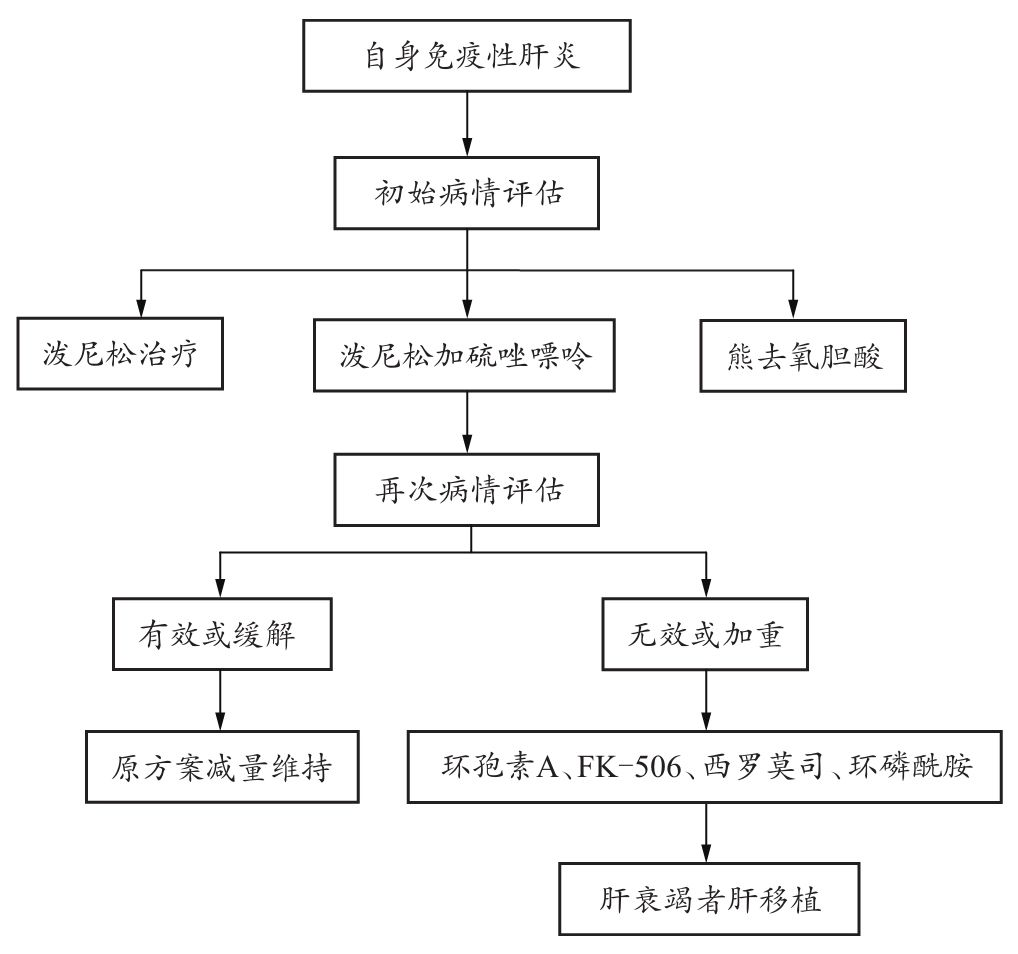
\includegraphics{./images/Image00100.jpg}
 \captionsetup{justification=centering}
 \caption{自身免疫性肝炎的治疗程序}
 \label{fig3-11-1}
  \end{figure} 

【治疗方案】

1.
治疗指针 符合下列条件的患者应予免疫抑制剂治疗:转氨酶明显升高(\textgreater{}正常上限10倍);转氨酶中度升高(\textgreater{}正常上限5倍)伴血清球蛋白明显升高(\textgreater{}正常上限2倍);组织学见桥状坏死或多小叶坏死。不符合上述条件者治疗视临床情况而定。

2. 药物治疗

(1)糖皮质激素对本病多有效,具体方法见表\ref{tab3-11-1}所示。

\begin{table}[htbp]
\centering
\caption{常规的治疗方法}
\label{tab3-11-1}
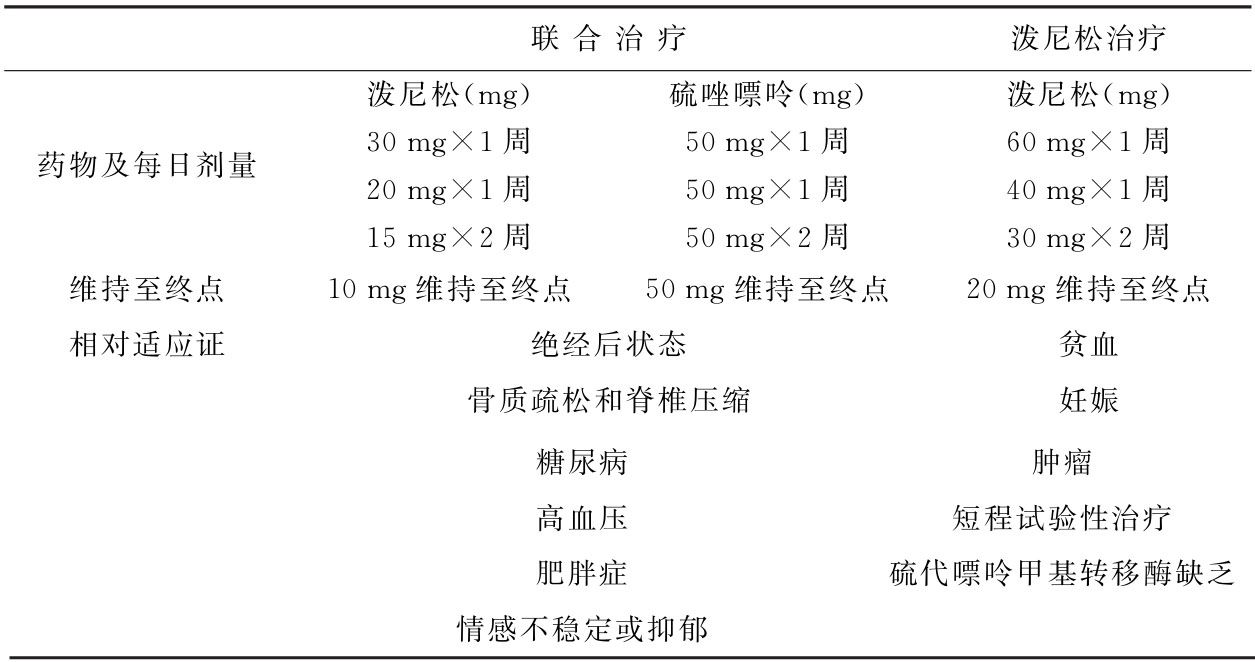
\includegraphics{./images/Image00101.jpg}
\end{table}

单用泼尼松疗法:第1周泼尼松60mg/d,第2周40mg/d,第3周、第4周30mg/d,第5周及以后20mg/d维持治疗。

泼尼松和硫唑嘌呤联合疗法:可提高疗效及减少不良反应。开始时用泼尼松30mg/d和硫唑嘌呤50mg/d,病情改善后逐渐减量至维持量泼尼松10mg/d和硫唑嘌呤50mg/d。

(2)大多数AIH患者对治疗反应较好,可长期存活。有20\%\textasciitilde{}40\%的患者无效。无效者可试用环孢霉素A、FK-506、西罗莫司、环磷酰胺等治疗。

(3)熊去氧胆酸(UDCA):具有免疫调节、保护肝细胞和去除脂溶性胆盐的作用,适用于轻症AIH或者无并发症患者的治疗,亦可用于治疗AIH/PBC重叠综合征患者。

(4)肝移植:少数治疗无效或已发生肝硬化患者最终发展为失代偿期肝硬化,晚期患者施行肝移植可提高存活率。

【疗效观察与随访】

1. 观察指标

(1)肝功能检查:在发病之初基本上所有患者都有血清转氨酶升高,转氨酶水平与肝坏死程度相关,但如果数值达几千则提示急性肝炎或其他疾病。胆红素和碱性磷酸酶多数轻到中度升高,碱性磷酸酶急剧升高常提示可能并发PBC或肝癌。

(2)免疫学检查:AIH患者血清γ球蛋白和IgG升高,其水平可反映患者对治疗的反应。自身抗体动态水平变化有助于评价病情、临床分型及指导治疗。这些抗体包括抗核抗体(ANA)、抗平滑肌抗体(SMA)、抗肝肾微粒体抗体(LKM1)、抗1型肝细胞溶质抗原抗体(LC1)、抗可溶性肝抗原抗体(anti-SLA)/抗肝胰抗体(anti-LP)、抗去唾液酸糖蛋白受体抗体(ASGPR)、抗中性粒细胞胞浆抗体(pANCA)。

(3)组织学检查:肝活检组织学检查有助于明确诊断及与其他疾病相鉴别。

2. 好转标准 症状改善,各项检测指标接近正常,半年内未见恶化。

3.
随访 注意病情观察,观察症状、肝功能等变化,避免肝损因素,并发症。AIH的预后差异较大,10年总体生存率为80\%\textasciitilde{}93\%。无症状患者预后较好,有症状患者13\%\textasciitilde{}20\%可能自发缓解。肝脏炎症程度影响着AIH的预后,初发就表现严重炎症的患者长期预后较差。治疗无法获得缓解或治疗后复发的预后也较差。多数患者最终仍发展为肝硬化。

【治疗经验与解析】

1. 临床分型对疗效的影响 AIH根据血清免疫学检查分型如下:

1型:以ANA和(或)SMA阳性为特征,SMA可能是小儿患者1型AIH的唯一标志。最常见,约占80\%,大部分为40岁以下女性。多数患者对免疫抑制剂的治疗效果好。

2型:特征为抗LKM1和(或)抗LC1阳性,仅约4\%可检测出ANA和(或)SMA。儿童多见,此型约占AIH的4\%。可快速进展为肝硬化,复发率高,对糖皮质激素的治疗效果较差。

3型:特征为抗-SLA及抗-LP阳性。激素治疗反应与1型相似。在ANA、SMA和抗LKM1自身抗体阴性患者中,抗-SLA/LP可能是唯一的标志。

4型:小部分AIH患者自身抗体阴性,可能存在目前尚不能检出的自身抗体,有人称之为Ⅳ型。Ⅳ型AIH与慢性隐源性肝病的区别是前者对糖皮质激素治疗有效,而后者多无效。

有些患者AIH可与其他自身免疫性肝病如原发性胆汁性肝硬化、原发性硬化性胆管炎等并存,称为重叠综合征。

2.
临床上AIH是以病情波动为特点,转氨酶并不是反映AIH患者潜在肝脏炎症坏死情况的可靠指标,对转氨酶水平正常或轻度升高的患者,肝组织学检查是决定是否需要治疗的最可靠指标。血清转氨酶水平正常但肝组织有明显桥形坏死或多小叶坏死的患者也需要激素治疗。经免疫抑制剂治疗,肝组织的改善往往落后临床及生化改善3\textasciitilde{}6个月,所以必须进行肝组织活检以确定组织学的缓解,防止过早停药。激素治疗的疗程至少2年,若病情仍未获得明显缓解则可停止治疗。激素治疗可在2年内使65\%的重度AIH患者病情获缓解。发病时无肝硬化者其治疗后5年和10年预期生存率超过90\%,而在已伴有肝硬化者其生存率分别为80\%和65\%。未治疗的重度AIH患者其3年和10年死亡率分别为50\%和90\%,显示激素治疗的疗效危险比有利于对重度AIH的治疗,但对中度和轻度AIH患者的疗效危险比尚不确定,所以对中度AIH的激素治疗需酌情决定,而对轻度AIH一般不列为治疗的指征。

3.
绝经后的妇女或伴有骨质疏松、不稳定性高血压、糖尿病或者情绪不稳定的AIH患者由于激素会加重这些患者副作用,因此需要采用激素和硫唑嘌呤的联合治疗方案,以减少激素用量。伴有贫血、妊娠以及儿童的AIH患者则不能应用硫唑嘌呤治疗,因此采用单用激素方案,但此时激素宜加量。肝硬化患者如炎症活动明显则可以采用联合治疗方案,但是需要考虑低蛋白血症和高胆红素血症对激素疗效的影响。对于以上这些特殊人群,必须加辅助治疗以预防或减轻激素副反应,严密监测药物相关的并发症。如规定适当的饮食、定期锻炼、及时调整激素的用量、补充钙和维生素D或给予一定量的二磷酸盐。

4.
常规治疗要持续进行直到疾病缓解。疾病缓解指症状消失,肝脏炎症的实验室指标改善(血清AST水平在正常值的2倍以内),组织学炎症的明显改善。治疗失败指临床、实验室或组织学的检查明显的恶化。实验室指标恶化主要是指血清AST水平明显升高。如果单独使用大剂量泼尼松(60mg/d)或者联合使用强的松(30mg/d)伴硫唑嘌呤(150mg/d)后血清AST水平仍明显升高则意味治疗失败,这时需要选择其他方法。13\%的激素治疗者会发生不良反应,系患者过早停药的原因之一。对有激素相关副作用的患者激素需减量,必要时需停药。硫唑嘌呤可以减少激素的用量,其副作用一般较少,主要有胆汁淤积、胰腺炎、皮疹、进行性血细胞减少等。出现以上表现则需停用硫唑嘌呤,同时调整泼尼松的剂量以抑制疾病的活动。经长期激素治疗后仍没达到理想的临床或实验室指标则表示激素治疗的不完全应答。不完全应答的发生率约为13\%,这时需评估激素治疗的疗效-危险比,低剂量泼尼松或硫唑嘌呤可以减轻激素的不良反应。

5.
复发指经治疗后病情减轻或停药后短期内又出现以下表现:患者血清AST升高至正常值的3倍以上伴易疲劳、关节痛等。复发须同激素停药后的症状相鉴别,后者的症状与复发相似但不伴有血清AST水平的异常。临床上复发多数与激素停药的治疗终点的标准有关,以肝组织学评估正常为治疗终点的患者的复发率仅为20\%,而治疗期间肝硬化进展或者在治疗结束时仍存在界面性肝炎的患者则大多会复发。此时采取再次治疗可以诱导疾病的再次缓解,由于易复发,因此低剂量泼尼松疗法或不限期的硫唑嘌呤疗法适合于这些患者。

低剂量泼尼松疗法指在临床和实验室指标好转的基础上,泼尼松的剂量按每月2.5mg递减直至能够控制症状并且维持血清AST水平在正常值5倍以内的最小剂量。大多数患者只需10mg/d或更少(7.5mg/d)的泼尼松来维持。不限期的硫唑嘌呤疗法指标准治疗后临床和生化指标明显改善,糖皮质激素减量,同时增加硫唑嘌呤量至2mg/(kg·d)并且一直维持。87\%的成年患者用这种方法治疗67个月后观察发现症状仍然减轻。94\%的随访肝脏活检表明疾病的组织学表现静止或处于炎症活动最轻状态。

\section{药物性肝病}

药物性肝病简称药肝,是指由于药物和(或)其代谢产物引起的肝脏损害。可以发生在以往没有肝病史的健康者或原来就有严重疾病的患者,在使用某种药物后发生程度不同的肝脏损害,均称药肝。目前至少有600多种药物可引起药肝,其表现与人类各种肝病的表现相同,可以表现为肝细胞坏死、胆汁淤积、细胞内微脂滴沉积或慢性肝炎、肝硬化等。

【治疗程序】 如图\ref{fig3-12-1}所示。

\begin{figure}[!htbp]
 \centering
 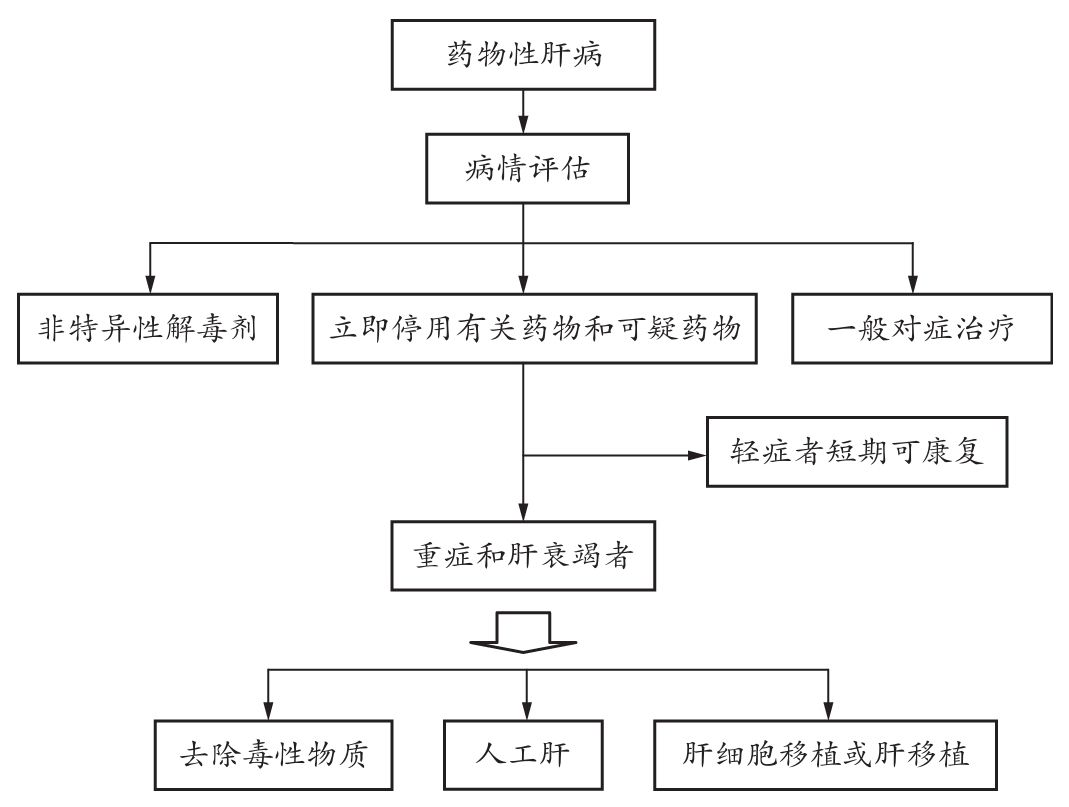
\includegraphics{./images/Image00102.jpg}
 \captionsetup{justification=centering}
 \caption{药物性肝病的治疗程序}
 \label{fig3-12-1}
  \end{figure} 

【治疗方案】

1. 一般治疗

(1)对药物性肝损害目前无特效治疗,但贵在早期识别。及时停药,肝损害大多能恢复。卧床休息,给予高维生素、高蛋白饮食。治疗的关键是停用和防止再使用引起肝损伤的药物,且也应尽可能避免使用与致病药物在生化结构和(或)药物作用属于同一类的药物。若同时或先后应用多种药物而无法确定致病药物,应首先停用最可疑药,若无法查出致病药物,停用全部药物。

(2)误服大量肝毒性药物的患者,宜早期洗胃、导泻,并加用吸附剂,以清除胃肠内残留的药物,可采取血液透析、利尿等措施,以促进其排泄和清除。加强支持疗法,维持内环境稳定,摄入足量热卡和蛋白质,维持水电平衡,补充多种维生素。因变态反应所致者,可同时采用抗过敏治疗。

2. 药物治疗

(1)根据不同肝损伤类型和机理进行药物治疗。对于直接肝毒性药物引起的肝损害,可应用特殊解毒剂(如还原型谷胱苷肽、乙酰半胱氨酸和葡萄糖醛酸内酯等);对于肝细胞性损伤者,可使用降酶药物(如甘草酸铵、联苯双脂、五味子、垂盆草等)和细胞膜稳定作用药物(如必需磷脂、硫普罗宁等)。

(2)对于明显淤胆型肝损伤可选用退黄为主药物(如熊去氧胆酸,门冬氨酸钾镁,苯巴比妥,腺苷蛋氨酸等)。对于防治肝损伤药物种类繁多,但多数药物的治疗效果尚需进行循证医学研究评价。各种保肝、利胆、降酶和护膜药物均可使用,酌情选用2\textasciitilde{}3种即可,但疗效难以肯定。

(3)糖皮质激素仅用于少数有特殊适应证(如胆汁淤积为主)的病例,不可滥用,宜短程给药(2周内)。

(4)根据肝损害的不同程度进行治疗。轻者在停药后或经一般对症处理后可很快好转,重者则需住院治疗。对于有明显临床表现和(或)出现中毒症状的患者,宜严密监护病情的发展。重症患者出现肝功能衰竭时,除积极监测和纠正其并发症外,建议采用人工肝支持疗法,对于预期有可能发生死亡的高危患者,应考虑肝移植治疗。

【疗效观察与随访】

1. 观察指标 肝功能监测、相关症状、体征、肝、胆、脾B超。

2.
治愈标准 症状、体征消失,肝功能恢复正常,肝B超检查恢复正常,病情稳定3个月以上。

3.
随访 注意病情观察,观察症状、体征等变化,避免肝损因素,防止肝衰竭,定期复查肝功能,必要时复查肝B超。

【治疗经验与解析】

1.
及时停药是决定治疗及预后的关键。大多数轻型反应者,病程具有自限性,只要停用致病药物,病情自然缓解。若同时或先后应用多种药物而无法确定致病药物,应首先停用最可疑药,若无法查出致病药物,可停用全部药物,如必须应用而不能去除时,应权衡利弊后做出选择,如抗结核药引发的轻微的ALT、AST升高一般不停药,如升高大于正常值的2倍或血清胆红素升高就应停药,再次用药待肝功能恢复正常以后,并在用药前和用药后每月监测肝功能。

2. 应给予对症支持治疗,以利于病情恢复。

3.
根据导致不良反应的药物,选用特殊解毒剂。因变态反应所致者,采用抗组胺药治疗。假膜性肠炎、真菌性肠炎以及药源性胰腺炎所致的继发感染等,应给予抗生素治疗或抗真菌治疗。

\section{酒精性肝病}

酒精性肝病是由于长期大量饮酒导致的肝脏疾病。初期通常表现为脂肪肝,进而可发展成酒精性肝炎、肝纤维化和肝硬化;严重酗酒时可诱发广泛肝细胞坏死甚至肝功能衰竭。根据临床表现,可分为轻症酒精性肝病、酒精性脂肪肝、酒精性肝炎、酒精性肝硬化。

【治疗方案】

1.
治疗目标 减轻酒精性肝病的严重程度,改善已存在的继发性营养不良和对症治疗酒精性肝硬化及其并发症。①戒酒是治疗酒精性肝病的最重要的措施,戒酒过程中应注意防治戒断综合征。②酒精性肝病患者需要良好的营养支持,应在戒酒的基础上提供高蛋白、低脂饮食,并注意补充维生素B、维生素C、维生素K及叶酸。

2. 药物治疗

(1)糖皮质激素:可改善重症酒精性肝炎(有脑病者或Maddrey指数\textgreater{}32)患者的生存率。可考虑给予为期4周的泼尼松治疗(40mg/d,持续28d,随后停药或在2周内逐步撤药)。

(2)美他多辛:可加速酒精从血清中清除,有助于改善酒精中毒症状和行为异常。

(3)抗炎保肝药物:腺苷蛋氨酸治疗可以改善酒精性肝病患者的临床症状和生物化学指标。多烯磷脂酰胆碱对酒精性肝病患者有防止组织学恶化的趋势。甘草酸制剂、水飞蓟素类、多烯磷脂酰胆碱和还原性谷胱甘肽等药物有不同程度的抗氧化、抗炎、保护肝细胞膜及细胞器等作用,临床应用可改善肝脏生物化学指标。双环醇治疗也可改善酒精性肝损伤。伴黄疸特别是胆汁郁积的患者,可选用熊去氧胆酸。但不宜同时应用多种抗炎保肝药物,以免加重肝脏负担及因药物间相互作用而引起不良反应。

(4)酒精性肝病患者肝脏常伴有肝纤维化的病理改变,故应重视抗肝纤维化治疗。

(5)积极处理酒精性肝硬化的并发症,如门静脉高压、食管胃底静脉曲张、自发性细菌性腹膜炎、肝性脑病等。

(6)严重酒精性肝硬化患者可考虑肝移植,但要求患者肝移植前戒酒3\textasciitilde{}6个月,并且无其他脏器的严重酒精性损害。

【疗效观察与随访】

1. 观察指标

(1)症状、体征:观察腹胀、腹痛、食欲不振、乏力的缓解情况,体重黄疸的好转状况。有神经精神症状和蜘蛛痣、肝掌等表现的注意观察变化。

(2)实验室检查:监测血清天冬氨酸氨基转移酶(AST)、丙氨酸氨基转移酶(ALT)、γ-谷氨酰转肽酶(GGT),总胆红素(TBil),凝血酶原时间(PT),平均红细胞容积(MCV)和缺糖转铁蛋白(CDT)等指标,禁酒后这些指标可明显下降,通常4周内基本恢复正常(但GGT恢复较慢)。肝、胆、脾B超亦为重要观察项目。

(3)评价酒精性肝病的严重程度及近期存活率:主要包括Child-Pugh分级、凝血酶原时间-胆红素判别函数(Maddrey判别函数)以及终末期肝病模型(MELD)积分等,其中Maddrey判别函数有较高价值,其计算公式为:4.6×(患者-对照)PT(秒)+总胆红素(mg/dl)。

2. 疗效评价 治愈标准:症状、体征消失,肝功能恢复至正常范围。

好转标准:仍存在肝脾肿大,肝功能虽有改善,但未能恢复到正常范围。

3.
随访 注意病情观察,避免并发症。除了对患者按时进行随访外,应注重对患者的教育,督促患者戒酒。定期复查肝功能、肝脾B超、血小板等。

【治疗经验与解析】

1.
酒精性肝病患者往往有酒精依赖。对酒精依赖患者采取精神治疗和药物治疗两方面。教育患者了解酒精对身体的危害及严重后果,使其逐渐减少饮酒量以至戒酒。必要时可酌情应用地西泮等镇静药物。且需注意热量、蛋白质、水分、电解质和维生素的补充。

2.
特殊情况下的药物治疗 对于合并HCV或HBV等肝炎病毒感染者,有学者建议戒酒至少6个月以上再开始抗病毒治疗。因为饮酒可妨碍对病毒性肝炎病情的观察,并使病毒性肝炎病情趋于恶化,降低抗病毒治疗的效果。在应用糖皮质激素治疗严重酒精性肝炎合并HBV或HCV等肝炎病毒感染的患者时,应权衡酒精性肝病的病死率与病毒复制增加之间的风险,慎用或不用。但有学者认为,糖皮质激素常规剂量、疗程4周以内,并不引起肝炎病毒复制的显著反弹。

\section{非酒精性脂肪肝}

非酒精性脂肪肝(Nonalcoholic fatty liver
disease,NAFLD)是指以肝实质细胞脂肪变性为病理特征,而无过量饮酒史,又除外其他肝病的临床综合征。其诊断标准为:①无饮酒史或饮酒折合乙醇量每周\textless{}140g(女性每周\textless{}70g)。②除外病毒性肝炎、药物性肝病、全胃肠外营养、肝豆状核变性、自身免疫性肝病等可导致脂肪肝的特定疾病。③病理组织学可见肝细胞脂变的基础上的肝细胞的损害,有多种炎性细胞浸润,常伴有小叶中央和叶间纤维化。

【治疗程序】 如图\ref{fig3-14-1}所示。

\begin{figure}[!htbp]
 \centering
 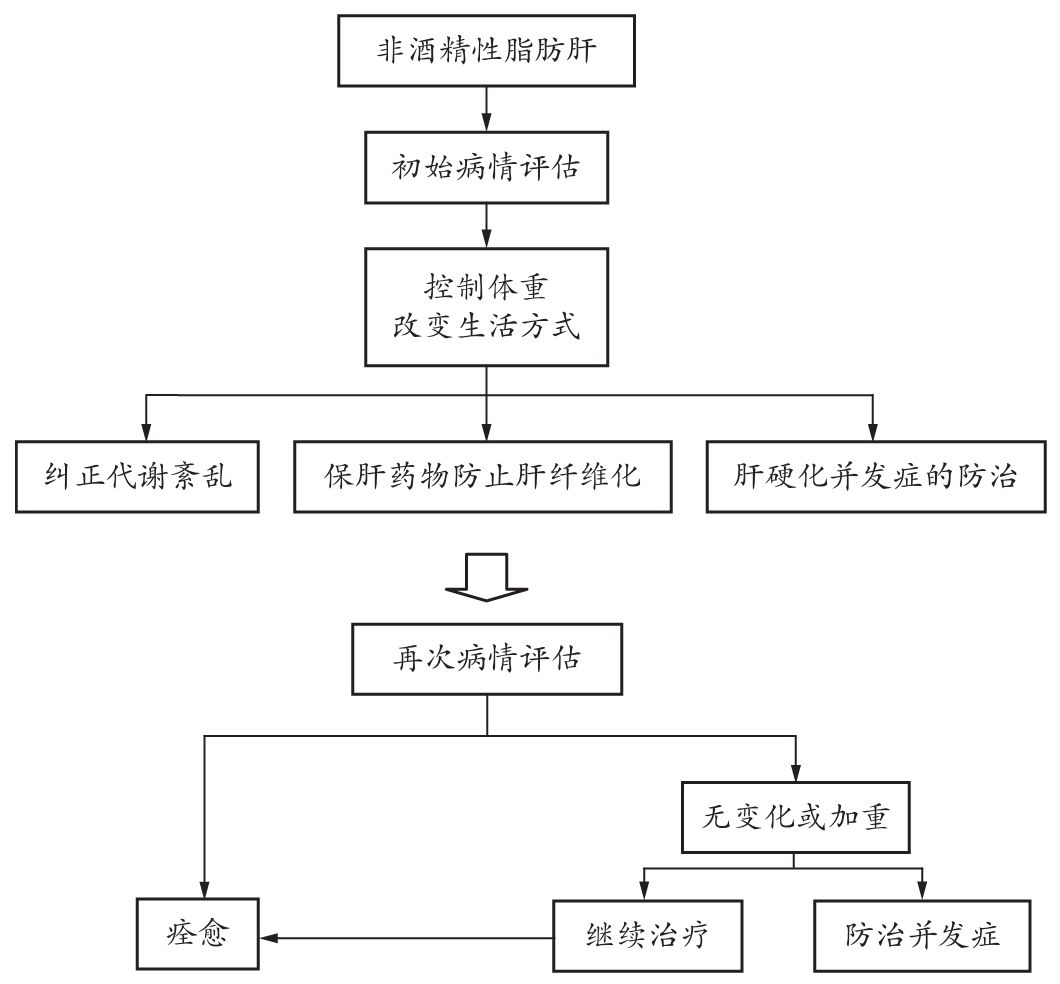
\includegraphics{./images/Image00103.jpg}
 \captionsetup{justification=centering}
 \caption{非酒精性脂肪肝的治疗程序}
 \label{fig3-14-1}
  \end{figure} 

【治疗方案】

1.
治疗目标 ①改善胰岛素抵抗,防止代谢综合征及相关器官终末期病变。②改善生活质量,延长生存时间。③减少肝脏脂肪沉积,避免二次打击,防止肝功能失代偿。④阻止肝病进展,减少或防止肝硬化、肝癌及并发症的发生。

2.
一般治疗 改变不良生活习惯及行为,改变饮食结构,中等量有氧运动,降低体重,减少腰围。

3. 药物治疗

(1)常用控制体重药物:对于改变生活方式6\textasciitilde{}12个月未能降低体重5\%以上的患者,可慎用二甲双胍、奥司利他等药物。

(2)改善代谢紊乱药物:血管紧张素受体阻滞剂、胰岛素增敏剂(吡格列酮、罗格列酮)、他汀类药物,降低血压、防止动脉硬化及糖脂代谢紊乱。

(3)保肝及抗肝纤维化药物:多烯磷脂酰胆碱、水飞蓟素、甘草酸制剂、还原谷胱甘肽、熊去氧胆酸、维生素E等,改善临床症状、降低转氨酶。

4. 肝硬化并发症的治疗 参见肝硬化章节。

【疗效观察与随访】

1.
观察指标 观察治疗后体重、体重指数、腰围、血压、肝功能、血脂、血糖及上腹部超声等。

2.
疗效评价 显效:体重不增加,稳定在标准体重范围内、血脂分析接近正常,半年内脂肪肝未加重。

3.
随访 除了对患者按时进行随访外,应注重对患者的教育。针对患者个体情况制定饮食、运动锻炼计划,并设立体重、腰围及相关生活质量检测指标的自我记录表。定期复查血脂、血糖、上腹B超、体重等,对超重者应结合计算体重指数。

【治疗经验与解析】

1.
使用改善代谢紊乱药物,降低血压及糖代谢的紊乱,能否改善血清酶谱的异常及肝组织学的异常尚无定论。

2.
保肝及抗肝纤维化药物可以改善临床症状、降低转氨酶,但没有足够证据证实可以改善肝组织学和延缓疾病进程。建议根据疾病活动度及病期以及药物的效能,合理选用1\textasciitilde{}2种药物,疗程通常需要6\textasciitilde{}12个月以上。

3.
加强生活调节,在医生指导下,适当进行体育锻炼,改变饮食结构,学会计算营养和热量,严格控制体重。

\section{肝硬化}

肝硬化(hepatic
cirrhosis)是各种慢性肝病发展的晚期阶段。病理上以肝脏弥漫性纤维化、再生结节和假小叶形成为特征。引起肝硬化病因很多,在我国以病毒性肝炎为主,欧美国家以慢性酒精中毒多见。临床上,起病隐匿,病程发展缓慢,早期可无症状或症状轻微,晚期以肝功能减退和门静脉高压为主要表现,常出现多种并发症。肝硬化是常见病,世界范围内的年发病率为25\textasciitilde{}400/10万,发病高峰年龄在35\textasciitilde{}50岁,男性多见,出现并发症时死亡率高。

【治疗程序】 如图\ref{fig3-15-1}所示。

\begin{figure}[!htbp]
 \centering
 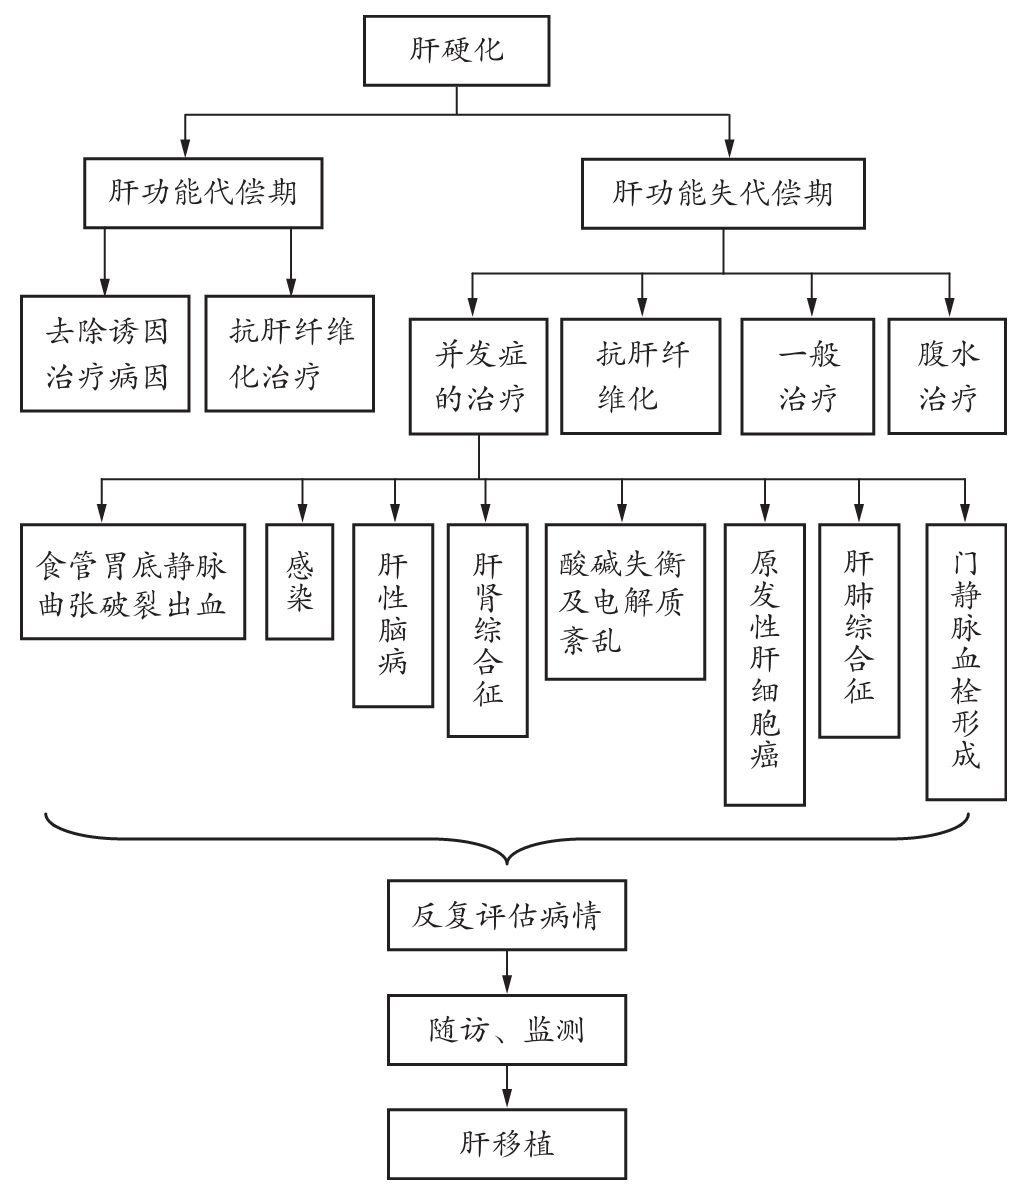
\includegraphics{./images/Image00104.jpg}
 \captionsetup{justification=centering}
 \caption{肝硬化的治疗程序}
 \label{fig3-15-1}
  \end{figure} 

【治疗方案】

1. 一般治疗

(1)休息:代偿期患者宜适当减少活动、避免劳累,失代偿期尤当出现并发症时患者需卧床休息。

(2)饮食:以高热量、高蛋白(肝性脑病时限制蛋白质饮食)和维生素丰富而易消化的食物为原则。盐和水的摄入视病情调整。禁酒,忌用对肝有损害药物。有食管静脉曲张者避免进食粗糙、坚硬食物。

(3)支持治疗:病情重、进食少、营养状况差的患者,应静脉纠正水电解质平衡,适当补充营养,视情况输注白蛋白或血浆。

2.
抗纤维化治疗 目前尚无有肯定作用的药物。治疗原发病,以防止起始病因所致的肝脏炎症坏死,可一定程度上起到防止肝纤维化发展的作用。对病毒复制活跃的病毒性肝炎肝硬化患者可予抗病毒治疗。

(1)慢性乙型肝炎:中华医学会肝病分会推荐治疗方案如下:

肝功能较好、无并发症的乙型肝炎肝硬化患者,HBeAg阳性者的治疗指征为HBVDNA≥10$^{5}$
拷贝/ml,HBeAg阴性者为HBV DNA≥10$^{4}$
拷贝/ml,ALT正常或升高。治疗目标是延缓和降低肝功能失代偿和HCC的发生。治疗药物为①拉米夫定100mg,每日1次口服,无固定疗程,需长期应用。②阿德福韦酯:对出现变异后病情加重的患者有较好效果,每日1次,10mg口服,无固定疗程,需长期应用。③干扰素:宜从小剂量开始,根据患者的耐受情况逐渐增加到预定的治疗剂量。因其有导致肝功能失代偿等并发症的可能,应十分慎重。

肝功能失代偿乙型肝炎肝硬化患者,治疗指征为HBV
DNA阳性,ALT正常或升高。治疗目标是通过抑制病毒复制,改善肝功能,以延缓或减少肝移植的需求。干扰素在肝功能失代偿患者禁忌使用。对于病毒复制活跃和炎症活动的肝功能失代偿肝硬化患者,在其知情同意的基础上,可给予拉米夫定治疗,但不可随意停药。一旦发生耐药变异,应及时加用其他能治疗耐药变异病毒的核苷(酸)类似物。

(2)慢性丙型肝炎:目前美国肝病学会推荐治疗方案如下:

1)肝功能代偿的肝硬化(Child-Pugh
A级)患者,建议在严密观察下给予抗病毒治疗。方案如下:

PEG-IFNα联合利巴韦林治疗方案:PEG-IFNα-2a
180μg每周1次皮下注射,联合口服利巴韦林1000mg/d,至12周时检测HCV
RNA:①如HCV
RNA下降幅度\textless{}2个对数级,则考虑停药。②如HCVRNA定性检测为阴转,或低于定量法的最低检测界限,继续治疗至48周。③如HCVRNA未转阴,但下降≥2个对数级,则继续治疗到24周。如24周时HCV
RNA转阴,可继续治疗到48周;如果24周时仍未转阴,则停药观察。

普通干扰素联合利巴韦林治疗方案:IFNα
3\textasciitilde{}5MU,隔日1次肌内或皮下注射,联合口服利巴韦林1000mg/d,建议治疗48周。

不能耐受利巴韦林不良反应者的治疗方案:可单用普通IFNα、复合IFNα或PEGIFN,方法同上。

2)肝功能失代偿肝硬化患者,多难以耐受IFNα治疗的不良反应,有条件者应行肝脏移植术。

3. 腹水的治疗

(1)限制钠和水的摄入:钠摄入量限制在60\textasciitilde{}90mmol/d(相当于食盐1.5\textasciitilde{}2g/d)。限钠饮食和卧床休息是腹水的基础治疗,部分轻、中度腹水患者经此治疗可发生自发性利尿,腹水消退。应用利尿剂时,可适当放宽钠摄入量。有稀释性低钠血症(\textless{}125mmol/L)者,应同时限制水摄入,摄入水量在500\textasciitilde{}1000ml/d。

(2)利尿剂 对上述基础治疗无效或腹水较大量者应使用利尿剂。临床常用的利尿剂为螺内酯和呋塞米。前者为潴钾利尿剂,后者为排钾利尿剂,主张两药合用,既可加强疗效,又可减少不良反应。先用螺内酯40\textasciitilde{}80mg/d,4\textasciitilde{}5日后视利尿效果加用呋塞米20\textasciitilde{}40mg/d,以后再视利尿效果分别逐步加大两药剂量(最大剂量螺内酯400mg/d,呋塞米160mg/d)。理想的利尿效果为每天体重减轻0.3\textasciitilde{}0.5kg(无水肿者)或0.8\textasciitilde{}1.0kg(有下肢水肿者)。使用利尿剂时应监测体重变化及血生化。

(3)提高血浆胶体渗透压:对低蛋白血症患者,每周定期输注白蛋白或血浆,可通过提高胶体渗透压促进腹水消退。

(4)难治性腹水的治疗:难治性腹水为使用最大剂量利尿剂(螺内酯400mg/d加上呋塞米160mg/d)而腹水仍无减退。表明患者对利尿剂反应差或不耐受,需辅以其他方法治疗。判定为难治性腹水前应首先排除其他因素对利尿剂疗效的影响并予纠正,如水钠摄入限制不够、严重的水电解质紊乱(如低钾、低钠血症)、肾毒性药物的使用、自发性腹膜炎、原发性肝癌、门静脉血栓形成等。难治性腹水的治疗可选择下列方法:

大量排放腹水加输注白蛋白:在1\textasciitilde{}2小时内放腹水4\textasciitilde{}6L,同时输注白蛋白8\textasciitilde{}10g/L,继续使用适量利尿剂。可重复进行。应注意不宜用于有严重凝血障碍、肝性脑病、上消化道出血等情况的患者。

自身腹水浓缩回输:将抽出腹水经浓缩处理(超滤或透析)后再经静脉回输,起到清除腹水,保留蛋白,增加有效血容量的作用。对难治性腹水有一定疗效。使用自身腹水浓缩回输前必须对腹水进行常规、细菌培养和内毒素检查,感染性或癌性腹水不能回输。不良反应包括发热、感染、DIC等。

经颈静脉肝内门体分流术(TIPS):是一种以血管介入的方法在肝内的门静脉分支与肝静脉分支间建立分流通道。该法能有效降低门静脉压,可用于治疗门静脉压增高明显的难治性腹水,但易诱发肝性脑病,故不宜作为治疗的首选。

肝移植:顽固性腹水是肝移植可考虑的适应证。

4. 并发症的治疗

(1)食管胃底静脉曲张破裂出血:

1)急性出血的治疗:死亡率高,急救措施包括防治失血性休克、积极的止血措施、预防感染和肝性脑病等。对食管胃底静脉破裂出血者应:①以三腔管气囊压迫。②通过胃镜或三腔管附管喷洒孟氏液、复方五倍子液或凝血酶以局部止血。③静脉用药止血:垂体后叶素,垂体后叶加压素或加压素与酚妥拉明或硝酸甘油并用以减少加压素的全身副反应。生长抑素或octreotide(善得定)静滴。临床应用表明,加压素与octreotide的止血作用相似。④食管静脉硬化治疗。内镜下行静脉瘤内或旁注入硬化剂。硬化剂常用的有鱼肝油酸钠、油酸苯乙醇胺、乙氧硬化醇等。⑤食管静脉内镜下结扎术。

2)预防再次出血:在第一次出血后,70\%的患者会再出血,且死亡率高,因此在急性出血控制后,应采取措施预防再出血。在控制活动性曲张静脉出血后,可以在内镜下对曲张静脉进行套扎。如果无条件作套扎,可以使用硬化剂注射。对胃底静脉曲张宜采用组织胶注射治疗。也可根据设备条件和医生经验联合使用上述内镜治疗方法。没有条件的地方可采用药物预防再出血。首选药物为β阻滞剂普萘洛尔,通过收缩内脏血管,降低门静脉血流而降低门静脉压力,普萘洛尔由10mg/d开始,逐日加10mg,逐渐加量至静息心率降为基础心率75\%左右,或心率不低于55次/分钟。普萘洛尔合用5-单硝酸异山梨醇酯可以更好降低门静脉压力。

3)预防首次出血:对中重度静脉曲张伴有红色征的患者,需采取措施预防首次出血。普萘洛尔是目前最佳选择之一,普萘洛尔治疗的目的是降低门静脉压力梯度至\textless{}12mmHg。如果普萘洛尔无效、不能耐受或有禁忌证者,可以慎重考虑采取内镜下食管曲张静脉套扎术或硬化剂注射治疗。

(2)自发性细菌性腹膜炎:合并自发性腹膜炎常迅速加重肝损害、诱发HRS、肝性脑病等严重并发症,故应早诊、早治。

1)抗生素治疗:选择对肠道革兰阴性菌有效、腹水浓度高、肾毒性小的广谱抗生素,以头孢噻肟等第三代头孢菌素为首选,可联合半合成广谱青霉素与β-内酰胺酶抑制药的混合物如舒他西林、替门汀等和(或)喹诺酮类药物,静脉给药,要足量、足疗程。一般于用药48小时复查腹水常规,如PMN减少一半以上可认为抗生素有效,继续至腹水白细胞恢复正常数天后停药。

2)静脉输注白蛋白:对发生HRS的高危患者(总胆红素\textgreater{}68.41μmol/L、血肌酐\textgreater{}88.4μmol/L)推荐开始用1.5g/(kg·d)、连用2日,继1g/(kg·d)至病情明显改善。

3)自发性腹膜炎的预防:急性曲张静脉出血或腹水蛋白低于1g/L为发生SBP高危因素,予氟喹诺酮类药物口服或静脉用药。

(3)肝性脑病:详见相关章节。

(4)肝肾综合征:积极防治HRS的诱发因素如感染、上消化道出血、水电解质紊乱、大剂量利尿剂等和避免使用肾毒性药物。合并自发性腹膜炎的肝硬化患者肝肾综合征发生率明显升高,除积极抗感染外及早输注足量白蛋白可降低肝肾综合征发生及提高生存率。近年研究证实下列治疗有可能改善肝肾综合征,疗法主要有:

1)血管活性药物加输注白蛋白:特利加压素加输注白蛋白对1型HRS的有效,用法为特利加压素每次0.5\textasciitilde{}1mg、每隔4\textasciitilde{}6小时1次,无效时可加量至最大12mg/d;白蛋白第1日1g/(kg·d)、继20\textasciitilde{}40g/d(若血白蛋白\textgreater{}45g/L或出现肺水肿时停用)。也有报道奥曲肽与α{2}
-受体拮抗剂合用,加输注白蛋白有一定疗效。

2)颈静脉肝内门体分流术(TIPS):有报道TIPS可促进HRS患者肾功能的恢复和难治性腹水的消退,并可提高1型肝肾综合征患者生存率,对药物治疗疗效欠佳的1型肝肾综合征患者如无禁忌可试用。

(5)肝肺综合征:目前无有效内科治疗,给氧只能暂时改善症状但不能改变自然病程。肝移植是唯一选择。

5.
门静脉高压症的手术治疗 主要是切断或减少曲张静脉的血流来源、降低门静脉压力和消除脾功能亢进,一般用于食管胃底静脉曲张破裂大出血各种治疗无效而危及生命者,或食管胃底静脉曲张破裂大出血后用于预防再出血特别是伴有严重脾功能亢进者。有各种断流、分流术和脾切除术等,手术预后与慎重选择病例和手术时机密切相关。在无黄疸或腹水、肝功能损害较轻者,手术预后较好;大出血时急诊手术、机体一般状况差、肝功能损害显著者,手术预后差、死亡率高。

6.
肝移植 是对晚期肝硬化治疗的最佳选择,掌握手术时机及尽可能充分做好术前准备可提高手术存活率。

【疗效观察与随访】

1.
观察指标 常见症状与体征、出血倾向、肝功能、肾功能、血清胆红素、血清蛋白、血小板、腹水常规及影像学检查,门静脉压力测定与急诊内镜检查等。

2.
疗效评价 好转:症状减轻、出血停止,黄疸消退或隐性黄疸,相关检测指标呈不同程度改善,病情稳定半年以上。

3.
随访 对肝硬化患者定期检查非常重要。乙肝患者和乙肝病毒携带者最好每半年作1次乙肝病毒检测、肝功能、AFP(甲胎蛋白)定量及B超检查,必要时还要作MRI或CT和胃镜检查,评估乙肝病毒的活动状态和肝功能代偿情况及有无肝癌等并发症。对有出血倾向者应定期复查出凝血指标;对有意识不清倾向者,应及时检测血氨,此外还应定期检查肾功能。

【治疗经验与解析】

1.
肝硬化在我国最常见的病因是病毒性肝炎,主要是乙型病毒性肝炎,其次为丙型肝炎,所以预防本病首先要重视病毒性肝炎的防治。早期发现和隔离患者给予积极治疗。

2. 注意饮食,合理营养,节制饮酒,加强劳动保健,避免各种慢性化学中毒。

3.
对有上述病因而疑有肝硬化者应及时进行全面体检及有关实验室检查,争取在代偿期得到合理积极治疗,防止向失代偿期发展。

4.
已确诊有肝硬化者,定期体格检查,包括检测肝功能、甲胎蛋白及肝胆胰脾超声波检查;同时避免各种诱因,预防和治疗食管、胃底静脉曲张破裂出血,原发性腹膜炎,肝性脑病(昏迷),肝肾综合征(少尿或无尿),肝癌等并发症,从而改善患者的预后。

5.
肝硬化病程长、病情复杂、治疗难度大。部分肝硬化晚期患者为了急于求效,多种药物一起用,结果增加了肝脏负担,使病情加重。

6.
肝硬化患者应合理饮食:①足够的糖类供应:糖类在饮食中比例占40\%,糖既保护肝脏,增强机体抵抗力,又减少蛋白质分解。②肝硬化患者蛋白质的补充应按蛋白质的缺乏程度及病情决定,能够进食的患者采用口服,而严重消化不良,吸收功能差者,应考虑输入氨基酸、蛋白和血浆。每天膳食中有60g高效蛋白可满足需要,可交替食用鱼、瘦肉、蛋类、乳类、豆制品。当有肝损倾向时,每天不宜超过20g。③肝硬化时,脂类代谢受到影响,同时脂类的代谢又可引起肝脏损伤,因此肝功能明显受损时,严格低脂肪饮食,减轻肝脏负担,加强补充蛋白和糖类,防止脂肪肝发生。④肝硬化由于多方面因素可造成维生素和微量元素的缺乏,新鲜蔬菜、水果含丰富维生素、矿物质、微量元素,是最好的食品。注意补充维生素B{1}
、维生素B{2}
、维生素C、维生素E和维生素K,微量元素如锌、硒,已出现维生素缺乏症状的应口服或肌内或皮下注射。⑤对腹水或水肿患者,一定要控制钠盐和水摄入量。⑥有食管胃底静脉曲张者,禁食硬食、油炸、粗纤维食物,以防损伤食道粘膜而出血。

\section{原发性肝癌}

原发性肝癌(primary carcinoma of the
liver,PLC)是指由肝细胞或肝内胆管上皮细胞发生的恶性肿瘤。是我国常见的十大恶性肿瘤之一,是目前各种实体瘤中预后最差的恶性肿瘤之一,其自然生存期仅为2\textasciitilde{}6个月。

【治疗程序】 如图\ref{fig3-16-1}所示。

\begin{figure}[!htbp]
 \centering
 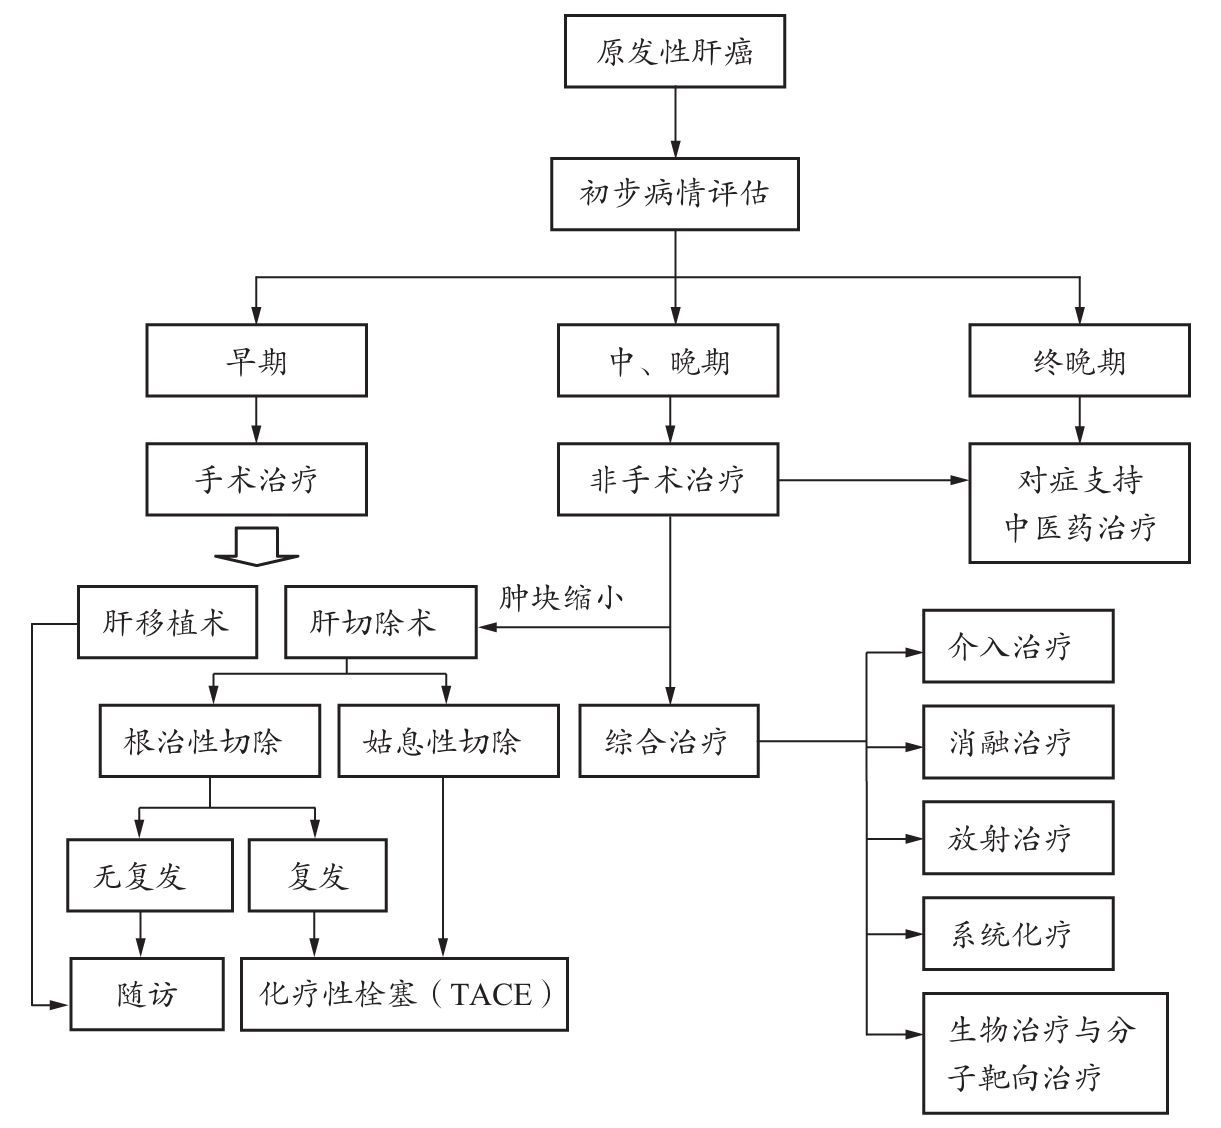
\includegraphics{./images/Image00105.jpg}
 \captionsetup{justification=centering}
 \caption{原发性肝癌的治疗程序}
 \label{fig3-16-1}
  \end{figure} 

【治疗方案】

1. 一般治疗 休息、注意保温、适当饮水。

2. 手术治疗 包括肝切除术和肝移植术。

(1)肝切除术:是目前根治原发性肝癌的最好手段,凡有手术指征者均应积极争取手术切除。肝切除方法包括根治性切除和姑息性切除。

肝癌手术适应证:

1)患者的一般情况(必备条件):一般情况良好,无明显心、肺、肾等重要脏器器质性病变;肝功能正常、或仅有轻度损害(Child-PughA级);或肝功能分级属B级,经短期护肝治疗后恢复到A级;肝储备功能基本在正常范围以内;无不可切除的肝外转移性肿瘤。

2)根治性肝切除的局部病变须满足下列条件:①单发肝癌,表面较光滑,周围界限较清楚或有假包膜形成,受肿瘤破坏的肝组织\textless{}30\%,或受肿瘤破坏的肝组织\textgreater{}30\%,但无瘤侧肝脏明显代偿性增大,达全肝组织的50\%以上。②多发性肿瘤,结节\textless{}3个,且局限在肝脏的一段或一叶内。

3)姑息性肝切除的局部病变须符合下列条件:①3\textasciitilde{}5个多发性肿瘤,超越半肝范围者,行多处局限性切除。②肿瘤局限于相邻2\textasciitilde{}3个肝段或半肝内,无瘤肝组织明显代偿性增大达全肝的50\%以上。③肝中央区(中叶或Ⅳ、Ⅴ、Ⅷ段)肝癌,无瘤肝组织明显代偿性增大达全肝的50\%以上。④肝门部有淋巴结转移者,肿瘤切除同时行淋巴结清扫或术后治疗。⑤周围脏器受侵犯者一并同时切除。

(2)肝移植术:用以治疗小肝癌特别是伴有肝硬化者,疗效较好,优于根治性切除术。对于局限性肝癌,如果合并肝硬化,肝功能失代偿(Child-Pugh
C级),且符合移植条件,应首选肝移植。肝移植术后进行适当的化疗及抗病毒治疗有可能减少肝癌复发、改善生存,但需要进一步研究。

3.
介入治疗 肝动脉化疗栓塞治疗(TACE)为原发性肝癌非手术治疗的首选方案,疗效好,可提高患者的3年生存率。TACE的主要步骤是经皮穿刺股动脉,在X线透视下将导管插至肝固有动脉或其分支,注射抗肿瘤药或栓塞剂。常用栓塞剂有明胶海绵碎片和碘化油。目前多采用碘化油混合化疗药,注入肝动脉,发挥持久的抗肿瘤作用。TACE应反复多次治疗,一般每4\textasciitilde{}6周重复1次,经2\textasciitilde{}5次治疗,许多肝癌明显缩小,可进行手术切除。另外,肝癌根治性切除术后TACE可进一步清除肝内可能残存的肝癌细胞,降低复发率。但对播散卫星灶和门静脉癌栓的疗效有限,更难控制病灶的远处转移。

4.
消融治疗 指影像技术引导下在局部直接杀灭肿瘤的一类治疗手段,目前以射频和微波消融及无水酒精注射最为常用。消融的途径可经皮肤入路,也可在腹腔镜手术或开腹手术中应用。影像引导手段主要包括超声和CT。常见消融手段有:射频消融(RFA)、微波消融(MWA)、无水酒精注射(PEI)、高强度聚焦超声消融(HIFU)。

(1)射频消融:是应用广泛的热消融手段。RFA对3\textasciitilde{}5cm的肿瘤具有根治率高、所需治疗次数少和远期生存率高的显著优势。射频消融存在导致针道转移、穿刺所致周围脏器损伤及诱发肝癌破裂等问题,此外也不适用于位于影像盲区的肝癌。

(2)微波消融:也是常用的热消融方法。MWA和RFA在局部疗效、并发症发生率以及远期生存方面都无显著差异。血供丰富的肿瘤,先凝固阻断肿瘤主要滋养血管,再灭活肿瘤可以提高疗效。

(3)无水酒精注射:适用于直径在3cm以内的小肝癌及复发小肝癌的治疗。对3cm以上不适合手术的肝癌或复发灶,也可起到姑息治疗的作用。

(4)高强度聚焦超声消融:与其他消融方法相比,HIFU是一种非侵入性的体外适形治疗肿瘤的新技术,疗效确切。目前认为,HIFU还不能作为PLC单独治疗模式,可以考虑作为TACE后进行补充治疗,或作为姑息治疗手段。

(5)其他:尚有醋酸注射治疗、冷冻治疗、激光治疗、电化学治疗等。

5.
放射治疗 由于放射源、设备的进步和定位方法的改进,如三维定向适形放疗,使放射治疗在肝癌治疗中地位有所提高。一些病灶较为局限、肝功能较好的早期病例,如能耐受40Gy(4000rad)以上的放射剂量,疗效可显著提高。目前趋向于用放射治疗联合化疗,如同时结合中药或其他支持疗法,效果更好。

6.
生物治疗与分子靶向治疗 生物治疗,特别是分子靶向治疗在控制HCC的肿瘤增殖、预防和延缓复发转移以及提高患者的生活质量等方面可能具有独特的优势;分子靶向药物治疗肝癌已成为新的研究热点,受到高度的关注。主要包括:①抗EGFR药物,如埃罗替尼和西妥昔单抗。②抗血管生成药物,如贝伐单抗和Brivanib等。③信号传导通路抑制剂,如mTOR抑制剂依维莫司。④多靶点抑制剂,如索拉非尼和舒尼替等。

7.
全身化疗 对肝癌较有效的药物以CDDP方案为首选,常用的化疗药物还有阿霉素、5-FU、丝裂霉素等,一般认为单一药物疗效较差。

8.
中医药治疗 中医以整体观念根据患者的全身特点辨证论治,可以适用于各型各期肝癌,尚在进一步探索中。

9.
肝脏移植 在肝硬化基础上发生的肝癌,早期行肝脏移植也是推荐的治疗方法。

【疗效观察与随访】

1.
观察指标 观察治疗前后症状以及体征变化。常规进行下列检查:三大常规、AFP+CEA+CA199、凝血功能、肝肾功能、肝炎十项、胸片、心电图、增强CT、肝胆彩超。肝切除术后1\textasciitilde{}2年内每1\textasciitilde{}2个月复查1次,2\textasciitilde{}5年每3月复查1次,5年后每半年复查1次。

2. 疗效评价 显效:术后症状,体征消失,5年内无复发。

3.
随访 介入治疗后随访期通常为35日至3个月,原则上为患者从介入术后恢复算起,至少持续3周以上。介入治疗的频率依随访结果而定,若介入术后1个月影像学检查肝肿瘤病灶内碘油沉积浓密,肿瘤组织坏死且无新病灶或无新进展,则暂不作介入治疗。治疗间隔应尽量延长,以保证肝脏功能的恢复。定期检查AFP、AFU、肝B超、肝功能、必要时检查肝CT。

【治疗经验与解析】

1.
影响疗效的重要因素包括肿瘤的大小和数目、肿瘤累及的部位和范围、门静脉癌栓与远处转移、肝功能代偿程度及全身状况。因此,必须重视PLC的早期发现和早期诊断,强调实施规范化综合治疗。

2.
由于患者个体差异和肿瘤生物学特性的不同,治疗过程要根据患者具体情况制定可行的治疗计划,合理地选择一种或多种治疗方法联合应用,尽可能去除肿瘤,修复机体的免疫功能,保护患者重要器官的功能。必须遵循循证医学的基本原则,并为PLC患者制定最佳的个体化治疗方案,避免不恰当或者过度治疗。

\section{肝性脑病}

肝性脑病(hepatic encephalopathy,HE)过去称为肝性昏迷(hepatic
coma),是由严重肝病引起的、以代谢紊乱为基础、中枢神经系统功能失调的综合征,其主要临床表现是意识障碍、行为失常和昏迷。临床分期:一期(前驱期)、二期(昏迷前期)、三期(昏睡期)、四期(昏迷期)。

亚临床性肝性脑病(subclinical hepatic
encephalopathy,SHE)又称为轻微肝性脑病,是指临床上患者虽无上述症状和体征,可从事日常生活和工作,但用精细的智力测验和(或)电生理检测可发现异常,这些患者的反应力常降低,不宜驾车及高空作业。

【治疗程序】 如图\ref{fig3-17-1}所示。

\begin{figure}[!htbp]
 \centering
 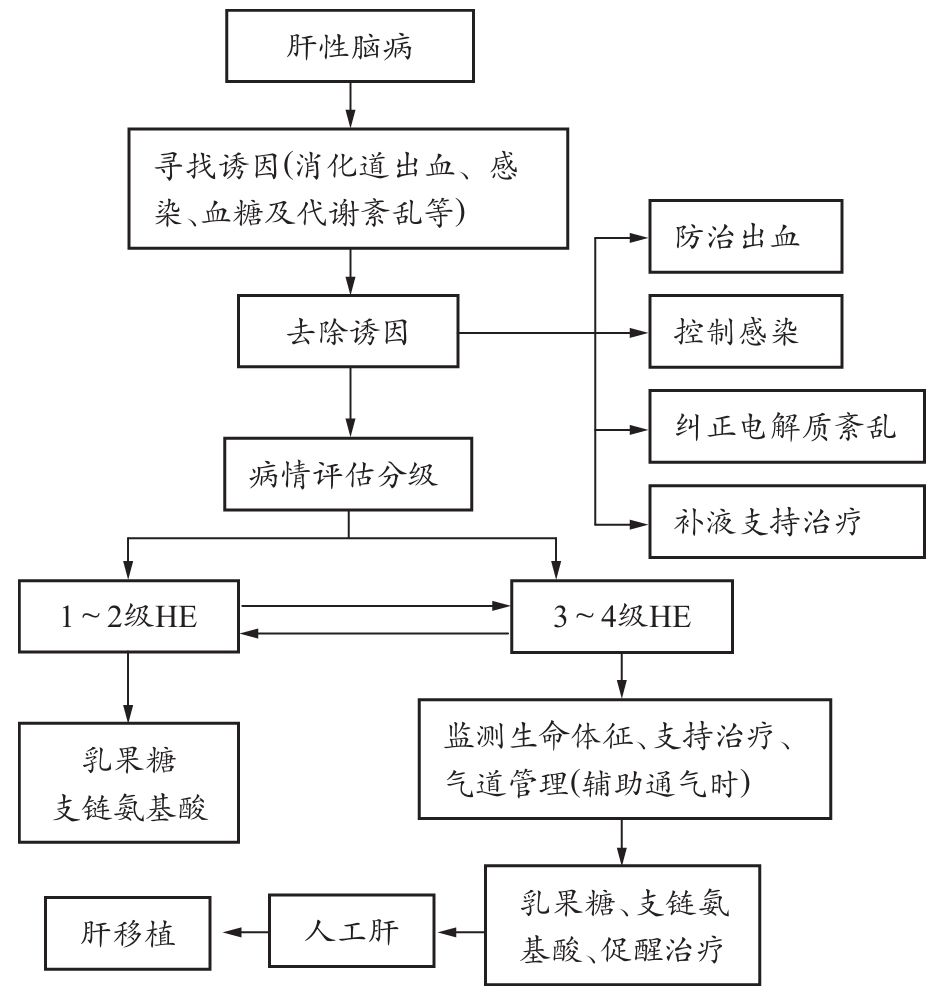
\includegraphics{./images/Image00106.jpg}
 \captionsetup{justification=centering}
 \caption{肝性脑病治疗程序}
 \label{fig3-17-1}
  \end{figure} 

【治疗方案】

1. 一般治疗

(1)治疗目的:去除HE发作的诱因、保护肝脏功能免受进一步损伤、治疗氨中毒及调节神经递质是治疗HE的主要措施。

(2)去除诱因:防治上消化道出血和感染最为重要,维持水、电解质及酸碱平衡,避免快速、大量排钾利尿和放腹水,避免使用巴比妥类及安定类药物,禁用吗啡类强力镇静药。

(3)营养疗法:发作性HE首日或昏迷患者暂禁蛋白。当神志开始转清后,可开始摄入小剂量蛋白,保持蛋白质摄入量40\textasciitilde{}60g/d,病情稳定或好转后渐增至每日1.0\textasciitilde{}1.5g/kg。首选植物蛋白和奶制品,口服补充支链氨基酸。

2. 药物治疗

(1)肠道降氨治疗:乳果糖的疗效确切,可用于各期肝性脑病及轻微肝性脑病的治疗。其剂量为每日30\textasciitilde{}60g,分3次口服,调整至患者每日排出2\textasciitilde{}3次软便。不良反应主要有腹胀、腹痛、恶心、呕吐等。亦可用乳果糖稀释至33.3\%保留灌肠。

(2)口服肠道不吸收抗生素:常用利福昔明,每日剂量为1.2g,15日为1疗程。新霉素的剂量为2\textasciitilde{}8g/d,分4次口服。口服新霉素很少吸收,但长期使用有可能致耳毒性和肾毒性,不宜超过1个月。

(3)降氨药物:对慢性反复发作的门体分流性脑病的疗效较好,对重症肝炎所致的急性肝昏迷无效。常用鸟氨酸门冬氨酸、谷氨酸钠、谷氨酸钾和盐酸精氨酸。

(4)支链氨基酸:包括支链氨基酸注射液、六合氨基酸注射液、肝安注射液等。

(5)中枢催醒治疗:常用氟马西尼、纳洛酮,氟马西尼对昏睡期HE及服用苯二氮@类HE有促清醒作用。

(6)微生态调节剂:益生菌是含有活菌或死菌(菌体成分及代谢成分)的生物制品,经口服可改善菌群失衡状态,减少氨和有毒物质的吸收并维持良好的肠粘膜屏障。

3.
MHE治疗策略 以营养疗法为基础,去除诱因为前提(以肝硬化食道胃底静脉曲张破裂出血和感染防治最为重要),肠、肝、脑为药物靶点,以智力检测为评估指标,旨在改善患者智能和生存质量。①更换工作,避免高空作业、驾驶等高危工种。②饮食疗法与HE相同,以植物蛋白摄入为主,均衡混合蛋白饮食。③小剂量乳果糖长程疗法被证实能显著改善MHE患者生存质量,逆转MHE自然病程,可使35\%的MHE患者免于恶化进展为临床肝性脑病,是迄今最有效的MHE疗法之一。④不能耐受乳果糖的患者可口服利福昔明或新霉素等不吸收抗生素,若仍无效可联用乳果糖和不吸收抗生素。⑤益生菌制剂同微生态调节剂治疗。

【疗效观察与随访】

1.
观察指标 观察患者意识、精神状态,神经肌肉的异常表现;脑电图、血气分析、血肌酐、血糖、血氨、血酮及电解质等检查。

2. 疗效判定

治愈标准:神志清醒,扑翼样震颤基本消失,性格行为恢复正常达3周以上。

好转标准:神志明显好转,但不巩固。

3.
随访 注意观察症状、体征、病情等变化,避免致病因素,避免并发症、后遗症。

【治疗经验与解析】

1.
避免和去除肝性脑病诱因是治疗肝性脑病最重要的措施,包括:①不适当的高蛋白饮食。②上消化道出血。③低血容量和低氧血症。④感染。⑤低钾碱中毒:呕吐、腹泻、大量利尿排钾、放腹水。⑥低血糖。⑦便秘。⑧氮质血症。⑨药物:如损肝药物、镇静药、催眠药。⑩麻醉与手术。

2.
饮食上从片面强调限摄蛋白向维持正氮平衡的方向进展,营养不良,负氮平衡会增加骨骼肌的动员,可导致继发性增加内源性蛋白质的分解而增高血氨含量,加重肝性脑病病情,故对肝性脑病患者营养处理的重点不是对蛋白质的限制,不可长时间禁食蛋白质。尽可能摄入可耐受的蛋白质。首选植物蛋白,以葡萄糖、支链氨基酸补充热量,保证每日的热量供给。

3.
口服肠道不吸收抗生素能有效抑制肠道产尿素酶细菌,减少氨生成和其他肠道毒素。常用新霉素、甲硝唑、万古霉素等。但长期服用有不良反应,药物长期使用的安全性限制了其广泛应用。目前这些药物多作为对口服不吸收双糖不能耐受或有抵抗患者的替代治疗,不作首选,更不主张长期应用。

4.
微生态制剂具有改善HE的作用,但目前仍存争议。服用不产生尿素酶的有益菌如乳酸杆菌、肠球菌、双歧杆菌、酪酸杆菌等,可抑制尿素酶细菌生长,乳果糖口服或者食醋灌肠,可酸化、清洁肠道,减少氨及其他毒素的吸收。

5.
抑制假性神经递质,纠正氨基酸失衡。支链氨基酸对于门体分流性肝性脑病有益,精氨酸可促进氨进入尿素循环,并可纠正代谢性碱中毒,可用于分流所致的肝性脑病。

6.
人工肝和肝移植是挽救患者生命的有效措施,人工肝支持系统可以代替肝脏的解毒功能,补充部分生物活性物质,过渡到肝移植。肝移植后1年生存率超过65\%。此外,肝细胞和骨髓干细胞移植尚处于试验阶段,已显示对于暴发性肝衰竭导致的肝坏死有替代作用,可改善生存率。

\section{胰腺炎}

\subsection{急性胰腺炎}

急性胰腺炎(acute
pancreatitis,AP)是多种病因导致胰酶在胰腺内被激活后引起胰腺组织自身消化、水肿、出血甚至坏死的炎症反应。临床上表现为急性、持续性腹痛(偶无腹痛),血清淀粉酶活性增高≥正常值上限3倍,影像学提示胰腺有或无形态改变,排除其他疾病者。可有或无其他器官功能障碍。少数病例血清淀粉酶活性正常或轻度增高。临床上常分为轻症与重症两型。

【治疗程序】

1. 轻症急性胰腺炎(MAP)治疗程序(图\ref{fig3-18-1})。

\begin{figure}[!htbp]
 \centering
 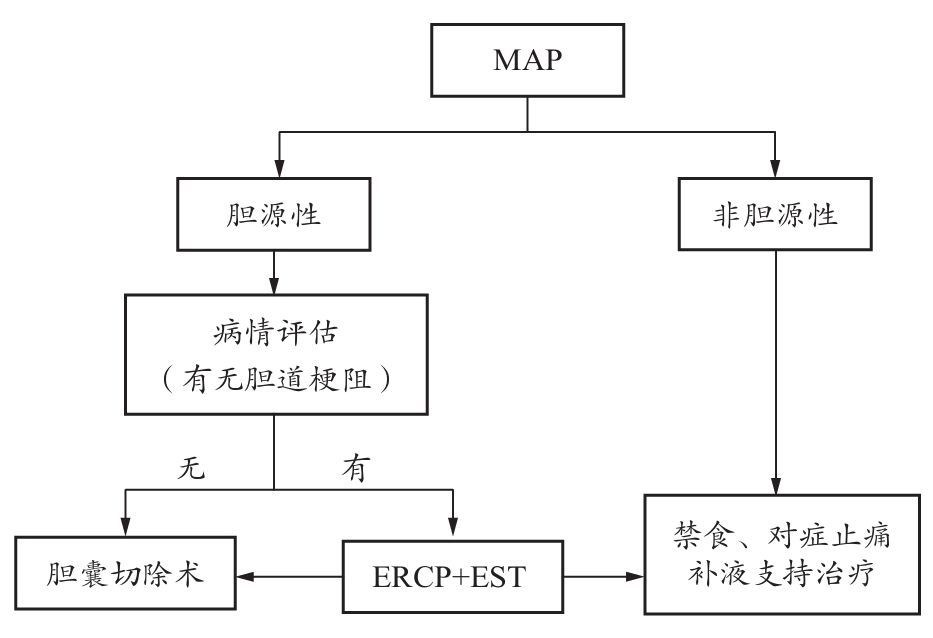
\includegraphics{./images/Image00107.jpg}
 \captionsetup{justification=centering}
 \caption{轻症急性胰腺炎治疗程序}
 \label{fig3-18-1}
  \end{figure} 

2. 重症急性胰腺炎(SAP)治疗程序(图\ref{fig3-18-2})。

\begin{figure}[!htbp]
 \centering
 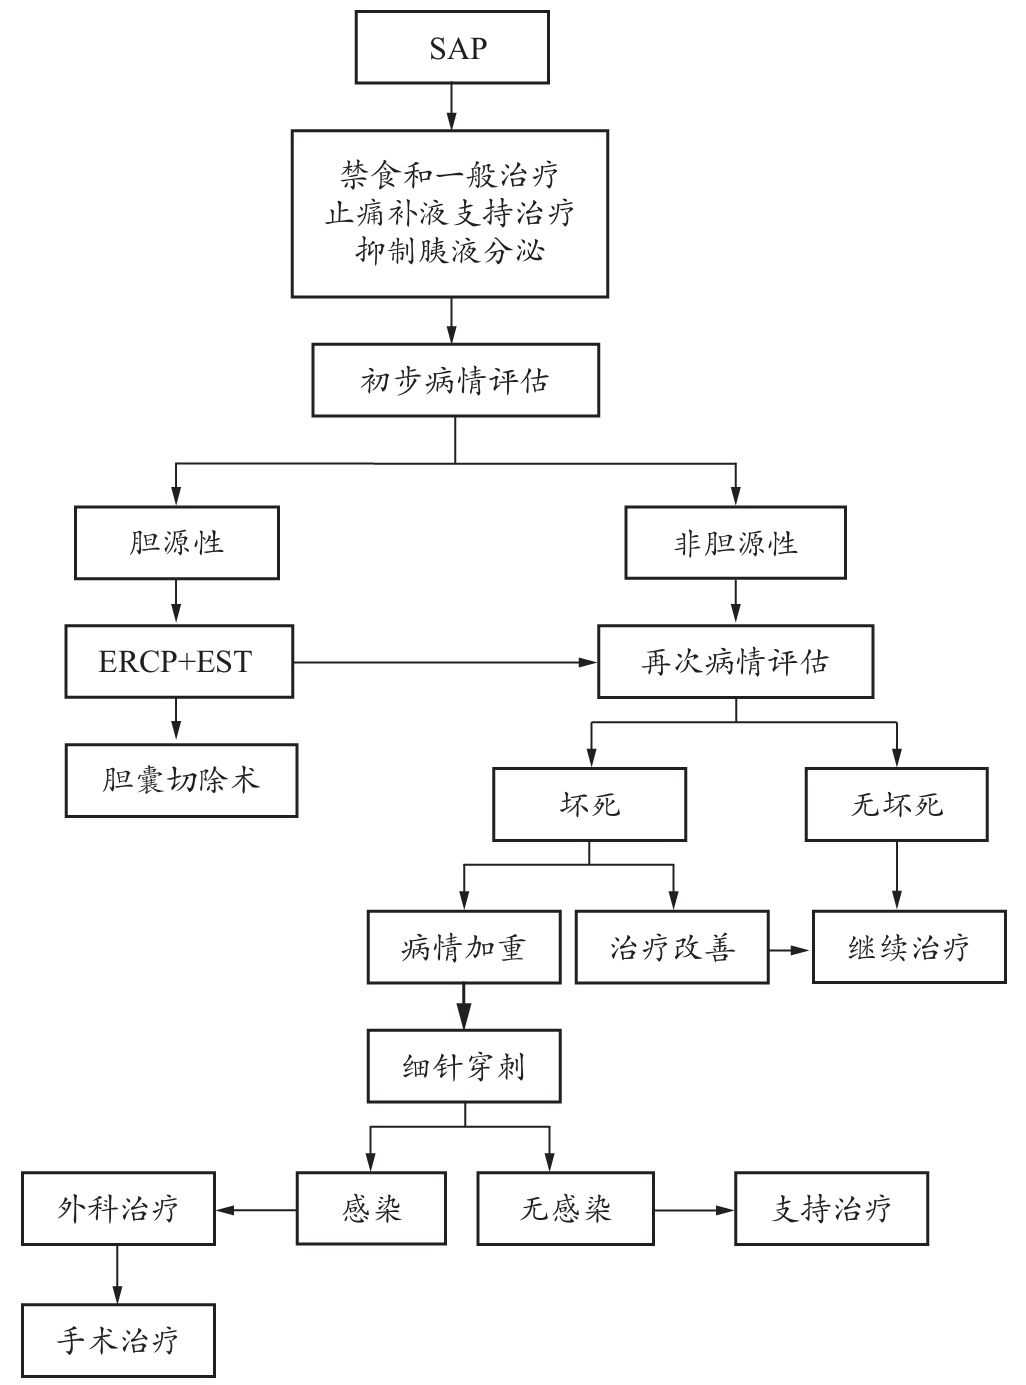
\includegraphics{./images/Image00108.jpg}
 \captionsetup{justification=centering}
 \caption{重症急性胰腺炎治疗程序}
 \label{fig3-18-2}
  \end{figure} 

【治疗方案】

1. 综合治疗

(1)一般治疗及监护:目的是纠正水、电解质紊乱,支持治疗,防止局部及全身并发症。常规禁食,对有严重腹胀,麻痹性肠梗阻者应进行胃肠减压。在患者腹痛、腹胀减轻或消失、肠道动力恢复或部分恢复时可以考虑开放饮食,开始以碳水化合物为主,逐步过渡至低脂饮食,不以血清淀粉酶活性高低作为开放饮食的必要条件。

(2)补液:补液量包括基础需要量和流入组织间隙的液体量。应注意输注胶体物质和补充微量元素、维生素。可酌情补充血浆、白蛋白、全血。

(3)镇痛:疼痛剧烈时考虑镇痛治疗。在严密观察病情下,可注射盐酸哌替啶(杜冷丁)。不推荐应用吗啡或胆碱能受体拮抗剂,如阿托品,654-2等,因前者会收缩奥狄氏括约肌,后者则会诱发或加重肠麻痹。

(4)营养支持:MAP患者只需短期禁食,故不需肠道或肠外营养。SAP患者常先施行肠外营养,待病情趋向缓解,则考虑实施肠内营养。应注意补充谷氨酰胺制剂。对于高脂血症患者,应减少脂肪类物质的补充。进行肠内营养时,应注意患者的腹痛、肠麻痹、腹部压痛等胰腺炎症状和体征是否加重,并定期复查电解质、血脂、血糖、总胆红素、血清白蛋白水平、血常规及肾功能等,以评价机体代谢状况,调整肠内营养的剂量。

2. 药物治疗

(1)胰腺外分泌抑制剂:生长抑素及其类似物(奥曲肽)可以通过直接抑制胰腺外分泌而发挥作用,主张在SAP治疗中应用。

(2)胰酶活性抑制剂:加贝酯可抑制蛋白酶、血管舒缓素、凝血酶原、弹力纤维酶等,根据病情,开始每日100\textasciitilde{}300mg溶于500\textasciitilde{}1500ml葡萄糖盐水,以2.5mg/(kg·h)速度静滴。2\textasciitilde{}3日后病情好转,可逐渐减量。

(3)抑酸治疗:H{2}
受体拮抗剂或质子泵抑制剂可通过抑制胃酸分泌而间接抑制胰腺分泌,同时可以预防应激性溃疡的发生,主张在SAP时使用。

(4)血管活性物质:由于微循环障碍在AP,尤其SAP发病中起重要作用,推荐应用改善胰腺和其他器官微循环的药物,如前列腺素E{1}
制剂、血小板活化因子拮抗剂、丹参制剂等。

(5)抗生素的应用:对于非胆源性MAP不推荐常规使用抗生素。对于胆源性MAP或SAP应常规使用抗生素。

(6)免疫增强剂应用:对于重症病例,可选择性应用免疫增强制剂。

(7)促肠道动力药物:包括生大黄、硫酸镁、乳果糖等。

(8)微生态制剂:调节肠道细菌菌群,应用谷氨酰胺制剂保护肠道粘膜屏障。

3.
中医中药 对急性胰腺炎有一定疗效。主要有柴胡、黄连、黄芩、枳实、厚朴、木香、白芍、芒硝、大黄(后下)等,随症加减。

4.
内镜治疗 适用于胆源性胰腺炎合并胆道梗阻或胆道感染者。行Oddis括约肌切开术和(或)放置鼻胆管引流。

5.
手术治疗 坏死胰腺组织继发感染者在严密观察下考虑外科手术。对于重症病例,主张在重症监护和强化保守治疗的基础上,经过72小时,患者的病情仍未稳定或进一步恶化,是进行手术治疗或腹腔冲洗的指征。手术适应证有:①胰腺坏死合并感染,在严密监测下考虑手术治疗,行坏死组织清除及引流术。②胰腺脓肿,可选择手术引流或经皮穿刺引流。③胰腺假性囊肿,视情况选择手术治疗、经皮穿刺引流或内镜治疗。④胆道梗阻或感染,无条件进行EST时予手术解除梗阻。⑤诊断未明确,疑有腹腔脏器穿孔或肠坏死者行剖腹探查术。

【疗效观察与随访】

1.
观察指标 动态观察腹部体征和肠鸣音改变。记录24小时尿量和出入量变化。行心电监护、血压监测。检测血、尿常规、粪便隐血、肝肾功能、血糖、血气分析、血清电解质尤其是血钙的水平测定以及C-反应蛋白(CRP)变化,注意监测血氧饱和度以及血气分析,必要时予胸部X线片,动态CT检查。

(1)早期病情预测:在发病早期,对病情严重程度进行预测,尽量减少并发症,达到最大治疗效果。

入院病情评估:患者入院后立即进行病情评估,重点在是否存在器官衰竭或心、肺、肾功能的不全表现。APACHEⅡ评分、体重指数、X线胸片、CT等。

入院24小时病情评估:重复临床评估和记录器官衰竭情况。评定24小时最差的APACHEⅡ评分,测定CRP值、进行Glasgow评分。

入院48小时病情评估:重复临床评估和记录器官衰竭情况。评定24小时最差的APACHEⅡ评分,测定CRP值、进行Glasgow评分。

(2)病情分级:区别轻症与重症胰腺炎十分重要,因两者的临床预后截然不同。有以下表现应当按重症胰腺炎处置:

临床症状:烦躁不安、四肢厥冷、皮肤呈斑点状等休克症状。

体征:腹肌强直、腹膜刺激征,Grey-Turner征或Cullen征阳性。

实验室检查:血钙显著下降2mmol/L以下,血糖\textgreater{}11.2mmol/L(无糖尿病史),血尿淀粉酶突然下降。

腹腔诊断性穿刺有高淀粉酶活性的腹水。

(3)APACHEⅡ评分标准:包括总生理分值12项,每项为1分。分为体温、平均动脉压、心率、呼吸、动脉血氧分压、血pH值、血钠、血钾、肌酐、血细胞比容、白细胞计数、昏迷积分。APACHEⅡ评分\textless{}8为MAP,≥8为SAP。

(4)Ranson评分标准:共计11项指标,每项1分,具体如下:入院时:年龄\textgreater{}55岁;WBC\textgreater{}16×10$^{9}$
/L;血糖\textgreater{}11.2mmol/L;血清LDH\textgreater{}350IU/L;AST\textgreater{}250IU/L。入院后48小时以内:红细胞压积下降\textgreater{}10\%;BUN升高\textgreater{}1.79mmol/L;血钙\textless{}2mmol/L;PaO{2}
\textless{}8kPa;碱缺乏\textgreater{}4mmol/L;估计体液丢失\textgreater{}6000ml。Ranson评分\textless{}3为MAP,Ranson评分≥3为SAP。

(5)Glasgow评分标准:每项1分,具体如下:48小时内,年龄超过55岁;WBC\textgreater{}15×10$^{9}$
/L;血糖\textgreater{}10.8mmol/L;LDH\textgreater{}600IU/L;BUN\textgreater{}16.065mmol/L;血清白蛋白\textless{}32g/L;血钙\textless{}2mmol/L;PaO{2}
\textless{}60mmHg。≥3为SAP。

(6)CT分级:根据炎症的严重程度分级为A\textasciitilde{}E级。CT分级为A、B、C为MAP,D、E为SAP。

A级:正常胰腺。

B级:胰腺实质改变,包括局部或弥漫的腺体增大。

C级:胰腺实质及周围炎症改变,胰周轻度渗出。

D级:除C级外,胰周渗出显著,胰腺实质内或胰周单个液体积聚。

E级:广泛的胰腺内、外积液,包括胰腺和脂肪坏死,胰腺脓肿。

A\textasciitilde{}C级:临床上为MAP;D\textasciitilde{}E级:临床上为SAP。

2.
治愈标准 症状、体征消失,相关检测指标正常1周以上。若尚有部分症状,但程度较轻为好转。

3. 随访和患者教育 注意病情观察,避免并发症,并予以及时处理。

【治疗经验与解析】

1.
适宜的支持治疗,积极的静脉液体补充对于纠正低血容量至关重要。低血容量可累及胰腺微循环,也是坏死性胰腺炎发生的主要原因。血容量减少导致血液浓缩、心动过速、低血压、尿量减少和肾前性氮质血症。早期的积极补液和改善氧供可防止或最小化胰腺坏死并提高生存率。

2.
如果存在持续性器官衰竭或其他胰腺炎重症化指征,如少尿、持续心动过速和劳力性呼吸困难,推荐将患者转入ICU。皮肤表现常发生在少数无痛性胰腺炎,可以作为首发症状,主要为脂肪坏死。

3.
因持续性器官衰竭或其他指征致不能摄食者需营养支持。营养支持可由全胃肠外营养或者行空肠营养。腹痛缓解,不需胃肠外麻醉剂,腹部压痛明显减轻,无恶心、呕吐,肠鸣音恢复,医生整体评价患者情况好转时一般开始摄入限定热量的食物。对于尚未确知胃肠营养开始之初能否安全接受低脂饮食或在低脂饮食之前应先接受清淡或流质饮食。

4.
坏死性胰腺炎患者不推荐预防性使用抗生素,依据近期前瞻性随机双盲研究显示其无益及长时间应用高效抗生素可能导致耐药Gram阳性菌或真菌感染。出现胰腺坏死的患者在发病的头7\textasciitilde{}10日及之后不同的住院时间均可能出现毒血症表现,如白细胞增多、发热和(或)器官衰竭。在寻找感染源的同时,予以经验性抗生素治疗是合理的。但如果血液及其他培养(包括CT引导细针抽吸培养)均阴性,无确认的感染源存在,推荐停止使用抗生素。

5.
早期奥迪括约肌切开术和取石(首选入院24小时内)对于重症急性胰腺炎和伴有上行性胆管炎的患者明显有益。ERCP早期干预能显著降低急性胆源性胰腺炎的并发症发生率,但死亡率无显著降低,对于存在胆总管结石和胆管炎的重症胆源性胰腺炎患者,有指征立即行ERCP和EST。

\subsection{慢性胰腺炎}

慢性胰腺炎以胰腺实质发生慢性持续性炎性损害、纤维化及可能导致的胰管扩张、胰管结石或钙化等不可逆性的形态改变为其特征,可引起顽固性腹痛和永久性内、外分泌功能损伤。

【治疗程序】 如图\ref{fig3-18-3}所示。

\begin{figure}[!htbp]
 \centering
 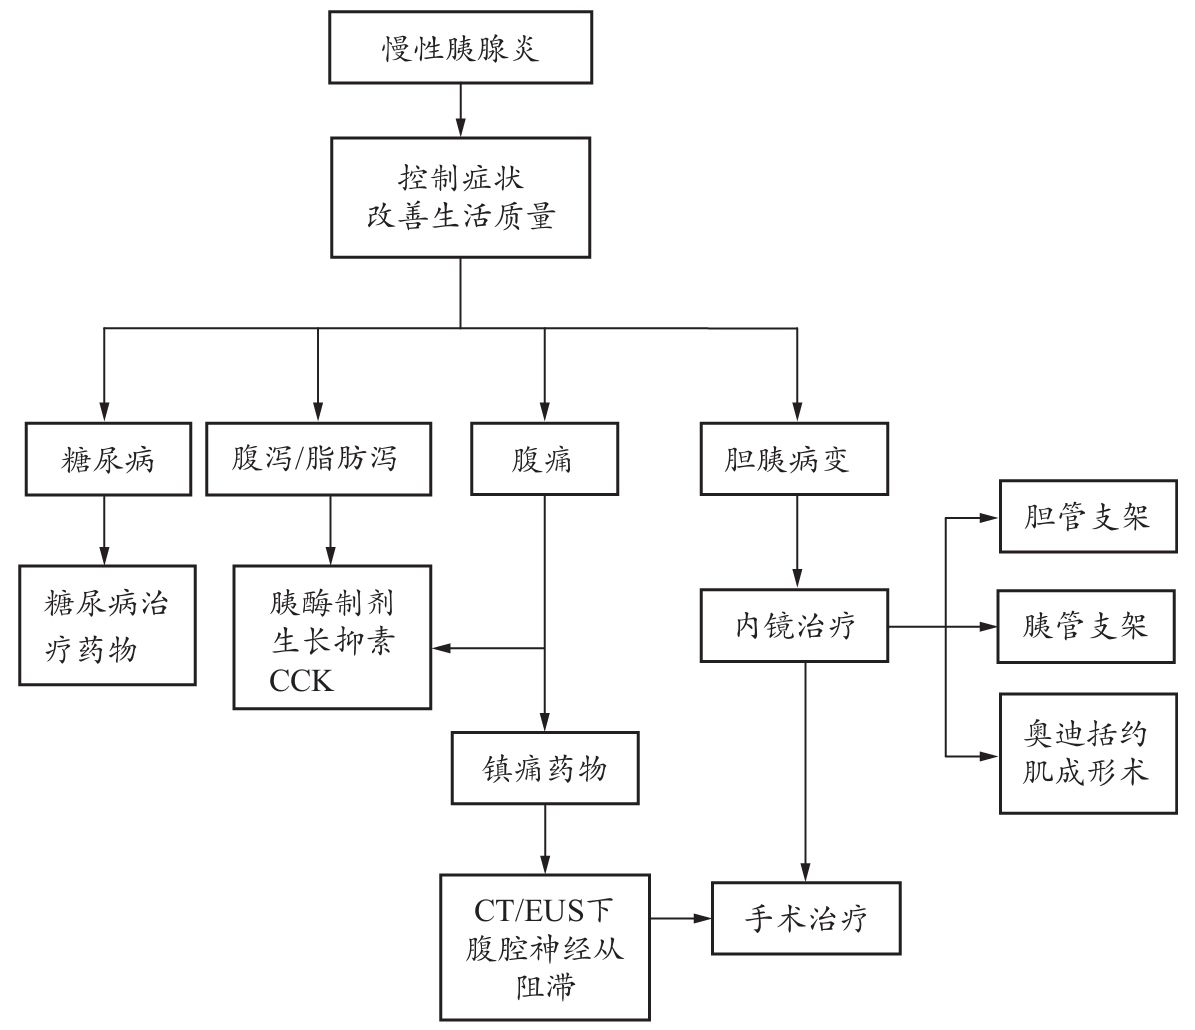
\includegraphics{./images/Image00109.jpg}
 \captionsetup{justification=centering}
 \caption{慢性胰腺炎的治疗程序}
 \label{fig3-18-3}
  \end{figure} 

【治疗方案】 治疗目的 包括缓解临床症状、改善营养状况和解决并发症,主要针对消化不良、疼痛和并发症等三个方面。

1.
对症治疗 ①胰腺外分泌功能不全导致的腹泻和脂肪泻:采用外源性胰酶制剂替代治疗,辅以饮食治疗。②发生糖尿病患者的治疗:按糖尿病的处理原则治疗。③疼痛治疗:治疗前须先对患者进行评估,如存在胰管梗阻因素和并发症等,非手术治疗则效果差,应转入外科治疗。

2.
药物治疗 应首选非镇痛药物,包括胰酶制剂、生长抑素及其衍生物和CCK拮抗剂。如果效果不好,可考虑使用镇痛药物,宜以醋氨酚和非甾体类抗炎药物开始,如果必要,可用曲马多或丙氧酚类的镇痛药物。只有在使用上述药物疼痛不能缓解或加重、或有并发症、或出现胃瘫方可使用麻醉性镇痛药物。以上方法不能获得疼痛缓解者,可以使用CT或EUS引导的腹腔神经从阻滞治疗。

3.
内镜治疗 主要用于慢性胰腺炎导致的奥迪括约肌狭窄(狭窄性十二指肠乳头炎)、胆总管下段狭窄和胰管开口狭窄和胰管结石。

(1)胆总管狭窄:发生率为10\%\textasciitilde{}30\%,主要表现为黄疸、淤胆性胆红素血症和胆管炎,影像学可以发现不同程度的胆总管扩张。可以首先考虑使用内镜支撑治疗,长期的疗效还不确定,但对年老和体弱的患者较为适用。

(2)胰管高压扩张:疼痛为主要症状的特发性、胰腺分裂症及其他原因的慢性胰腺炎是经内镜胰管支撑治疗的适应证。近期疼痛缓解较好,长期的疗效还不确定。

(3)奥迪括约肌功能不良和胰管结石:奥迪括约肌成形术治疗奥迪括约肌功能不良,短期止痛效果较好。对有主胰管结石的患者,可以尝试内镜下ERCP取石。

4.
手术治疗 早、中期干预可能会延缓胰腺实质的改变和保护内、外分泌功能。主要治疗成功的标志是疼痛的缓解或发作频率和程度的下降。

手术指征包括:①内科处理不能缓解的疼痛。②胰管结石、胰管狭窄伴胰管梗阻。③发生胆道梗阻、十二指肠梗阻、门静脉高压和胰性腹水或囊肿等并发症。

手术治疗的原则是采用尽可能简单的术式缓解疼痛、纠正并发症和提高生活质量,手术中应尽可能少的切除胰实质以避免糖尿病和外分泌功能不足。

手术方法有胰管纵行切开减压胰肠侧侧吻合术、各类胰头切除术、胰腺远端切除术、胰十二指肠切除术、全胰切除术、自体胰岛移植、胰腺支配神经切断术及针对病因的有关手术等。

【疗效观察与随访】

1. 观察指标 常见症状与体征、血或尿淀粉酶、血象及上腹部B超等。

2.
治愈标准 症状与体征消失,相关检测指标正常,无并发症。若仍有部分症状,时有发作为好转。

3.
随访 加强恢复期患者教育,注意病情观察。定期复查血尿淀粉酶,上腹部B超。

【治疗经验与解析】

1.
本病早期症状并不特异,当出现典型腹痛和(或)消化不良时,胰腺已经存在严重不可逆的结构和功能损害,因而要重视早期诊断和治疗。

2.
内镜下治疗逐渐成为处理本病各种并发症首选的重要手段。对于胰腺假性囊肿、胰管狭窄、胰管结石均可采用内镜下治疗。经内镜十二指肠乳头括约肌或胰管括约肌切开、副乳头切开、胰管括约肌扩张胰管支架置入,可解除胰管梗阻,减轻胰管内压力,从而缓解本病的疼痛。

3.
本病治疗非常复杂,不同治疗手段各有利弊,需要临床医生结合患者的个体情况综合判断,进行恰当选择,有时甚至需要多种方法结合应用,做到个体化治疗。

\section{胰腺癌}

胰腺癌主要指胰外分泌腺的恶性肿瘤,发病率近年来明显上升,恶性程度高、发展较快、预后较差。临床上主要表现为腹痛、食欲不振、消瘦和黄疸等。发病年龄以45\textasciitilde{}65岁最多见,男女之比为1.58∶1。胰腺癌的病因尚不十分清楚。胰腺癌可发生在胰腺的任何部位,但发生在胰头者更为多见,发生于胰头者较体尾部约多1倍。即胰头癌占60\%\textasciitilde{}70\%,胰腺体尾占25\%\textasciitilde{}30\%。在体部约为20\%,而尾部仅占5\%左右。

【治疗程序】 如图\ref{fig3-19-1}所示。

\begin{figure}[!htbp]
 \centering
 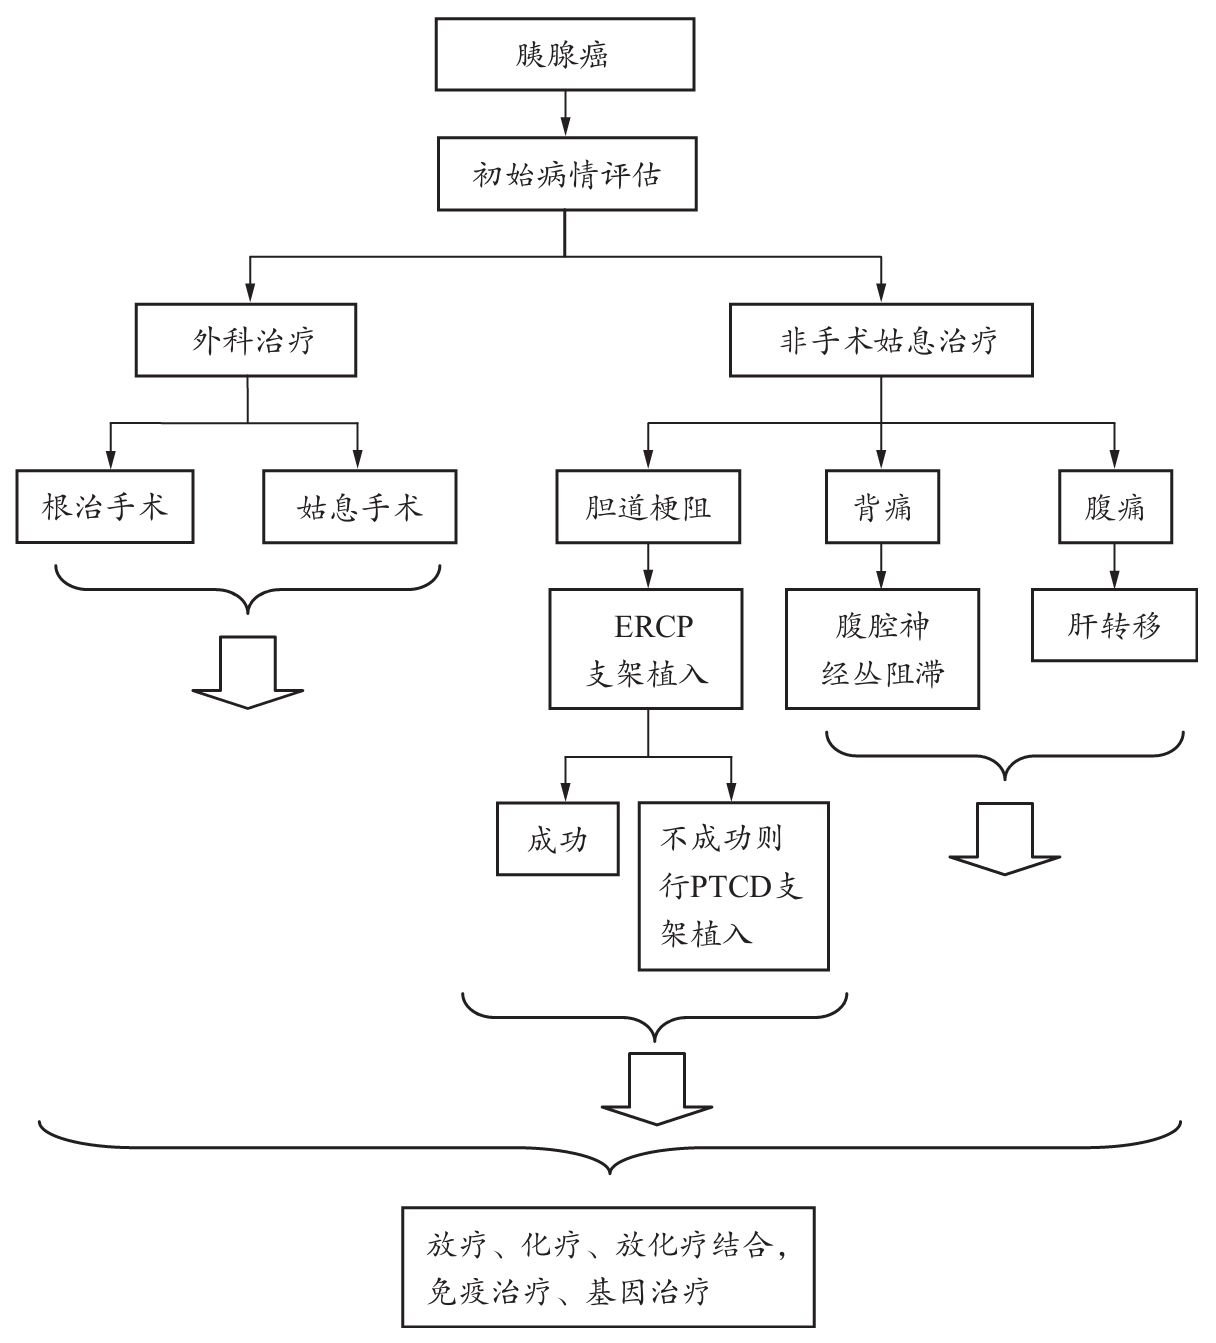
\includegraphics{./images/Image00110.jpg}
 \captionsetup{justification=centering}
 \caption{胰腺癌的治疗程序}
 \label{fig3-19-1}
  \end{figure} 

【治疗方案】

1.
一般治疗 应用各种支持疗法对晚期胰腺癌及术后患者均十分重要,可选用静脉高营养和氨基酸液输注,改善营养状况;可给予胰酶制剂治疗消化吸收功能障碍;有阻塞性黄疸时补充维生素K;治疗并发的糖尿病或精神症状等。

对有顽固性腹痛者可给予镇痛及麻醉药,必要时可用50\%乙醇或神经麻醉剂作腹腔神经丛注射或行交感神经节阻滞疗法,腹腔神经切除术。也可硬膜外应用麻醉药缓解疼痛。

2. 放射治疗

(1)辅助放疗:手术切除后,不论切缘或淋巴结状态都可采用,可与化疗联合。照射的靶区根据术前CT和(或)术中CT标记,应包括原发肿瘤或瘤床和局部淋巴结。建议采用三维适形放疗。剂量为40\textasciitilde{}50Gy(1.8\textasciitilde{}2Gy/d)。

(2)姑息性放疗:可与化疗联合。照射的靶区根据CT或术中标记,应包括原发肿瘤和局部淋巴结。建议采用三维适形放疗。剂量为40\textasciitilde{}50Gy(1.8\textasciitilde{}2Gy/d)。

3. 化疗

(1)辅助化疗:根治性手术切除后予以吉西他滨1000mg/m{2}
,第1、8、15日,连用6个周期。

(2)姑息性化疗:吉西他滨1000mg/m{2}
,第1、8、15日,至病灶进展或出现不可耐受的不良反应。

局部病灶残留或切缘阳性者术后予以含5-FU或吉西他滨的同期辅助放化疗(放疗剂量为40\textasciitilde{}54Gy)。

胰腺癌伴转移一线标准方案:吉西他滨1000mg/m{2}
,30分钟滴注,每周1次,连续3周,28日为1个周期,共2\textasciitilde{}3个周期;对伴有肝转移者可包含肝动脉化疗;有胰腺原发病灶者,如一般状况好,化疗同期予以胰腺的姑息性局部治疗[超声聚焦刀和(或)放疗]。

局部进展无法切除胰腺癌:同期放化疗(5-FU+放疗/吉西他滨+放疗)和(或)超声聚焦刀治疗为标准方案;同期放化疗结束后病情未进展可以吉西他滨化疗作为延续方案继续应用,对于无法行放疗和(或)超声聚焦刀治疗者可以吉西他滨化疗作为替代方案,共化疗2\textasciitilde{}3个周期。

吉西他滨可用固定剂量速率[10mg/(m{2} ·min)]法代替30分钟滴注法。

一般状况好,或患者要求可选用包含吉西他滨的联合化疗方案:一线化疗2个疗程后病情进展,或治疗后任何时间出现复发、转移、进展,可采用二线化疗:未用过吉西他滨者可予以包含吉西他滨的方案,已用过吉西他滨者可用卡培他滨(1000mg/m{2}
口服,每日2次,第1\textasciitilde{}14日,每21日重复)或静脉持续5-FU灌注200\textasciitilde{}250mg/(m{2}
·d);或改用动脉灌注或栓塞化疗。

适应证:①发现时伴有肝转移的胰腺癌。②胰腺癌手术或其他治疗后出现肝转移。③无法切除胰腺癌全身化疗失败者。

肝动脉化疗方案:

吉西他滨1000mg/m{2} +顺铂60mg/m{2}

吉西他滨1000mg/m{2} +奥沙利铂135mg/m{2}

肝转移灶富血供者同时适当予以肝动脉(或肝转移灶供血动脉)超液化碘油栓塞治疗,用量根据肿瘤大小、血管直径及患者耐受程度而定,联合化疗者可将化疗药物与碘油混合为乳剂进行栓塞。

全身化疗失败可改用腹腔动脉、肝动脉或肠系膜上动脉(视肿瘤供血动脉而定)化疗。

有胰腺原发病灶者,动脉化疗后予以胰腺的姑息性局部治疗[放疗和(或)超声聚焦刀]。

4. 中医中药辨证施治

5. 生物靶向治疗

(1)IL-2:NS 250ml+IL-2
20万\textasciitilde{}60万U,ivgtt,qd;4周为1个疗程,休息2\textasciitilde{}4周后重复;或qod,8周为1个疗程,休息2\textasciitilde{}4周后重复。

(2)胸腺肽:NS
250ml+胸腺肽40\textasciitilde{}200mg,ivgtt,qd;4周为1个疗程,休息2\textasciitilde{}4周后重复;或qod,8周为1个疗程,休息2\textasciitilde{}4周后重复。

(3)α-干扰素:100万\textasciitilde{}300万U,im,qod或biw;8周为1个疗程,休息2\textasciitilde{}4周后重复。

【疗效观察与随访】

1. 观察指标

(1)症状、体征:观察腹痛、发热、体重减轻的情况,黄疸、各种消化道症状,如食欲不振和消化不良、脂肪泻、上消化道出血等。精神忧郁、焦虑、个性改变等精神症状。可出现胰源性糖尿病或原有糖尿病加重。有时出现血栓性静脉炎的表现。

(2)肿瘤标志物检测:尚无一种理想筛选早期胰腺癌的肿瘤标志物。

(3)影像学检查:B超是胰腺癌的首选无创性检查。对于B超发现有异常者或者显示不清者应进一步进行CT或MRI检查,可进一步显示胰腺肿块的位置、大小、密度以及有无胰管和(或)胆管扩张、病灶的局部浸润、淋巴结转移情况以及是否伴有肝转移。对于CT和(或)MRI诊断不能明确的可考虑行ERCP。

(4)组织病理学和细胞学检查:在CT、B超定位和引导下,或在剖腹探查中用细针穿刺作多处细胞学或活体组织检查,确诊率高。

2. 疗效评价 治愈标准:术后症状、体征消失,无手术并发症,5年无复发。

3. 随访 注意病情观察,观察症状、体征等变化,早期处理并发症。

【治疗经验与解析】

1.
肿瘤相关抗原CA19-9水平\textgreater{}1000U/ml时诊断胰腺癌的准确性大于90\%。CA19-9同样可用来判断预后及治疗过程监测。CA19-9通常表达于胰腺和肝胆疾病及其他许多恶性肿瘤,虽然它不是肿瘤特异性的,但是CA19-9的上升水平对于胰腺癌与胰腺炎性疾病的鉴别很有帮助,而且CA19-9水平的持续下降与手术或化疗后的胰腺癌患者的生存期有关。

2.
胰腺癌术前及术后化疗和(或)放疗仍然存在争议,与5-FU相比,吉西他滨(Gemcitabine)在提高生存质量方面略显优势。分子靶向药物的疗效正在评估中。吉西他滨单药治疗是金标准,也可联合卡培他滨或澳铂、或TKI厄罗替尼化疗,若患者一般情况较好,可化放疗联合。放疗包括术前放疗、术中放疗、适形调强放疗、放射性核素内照射治疗和放化疗。随着放疗技术不断改进,胰腺癌的放疗效果有所提高,常可使症状明显改善,存活期延长。中医中药及免疫治疗可起到一定的辅助治疗作用。

\section{胆石症与胆囊炎}

\subsection{胆石症}

胆石症是指胆道系统(包括胆囊和胆管)任何部位发生结石的疾病。其临床取决于结石是否引起胆道感染、胆道梗阻及梗阻的部位和程度。按发生的部位来分,可分为胆囊结石、肝外胆管结石和肝内胆管结石。

【治疗程序】

1. 胆囊结石的治疗程序(图\ref{fig3-20-1})

\begin{figure}[!htbp]
 \centering
 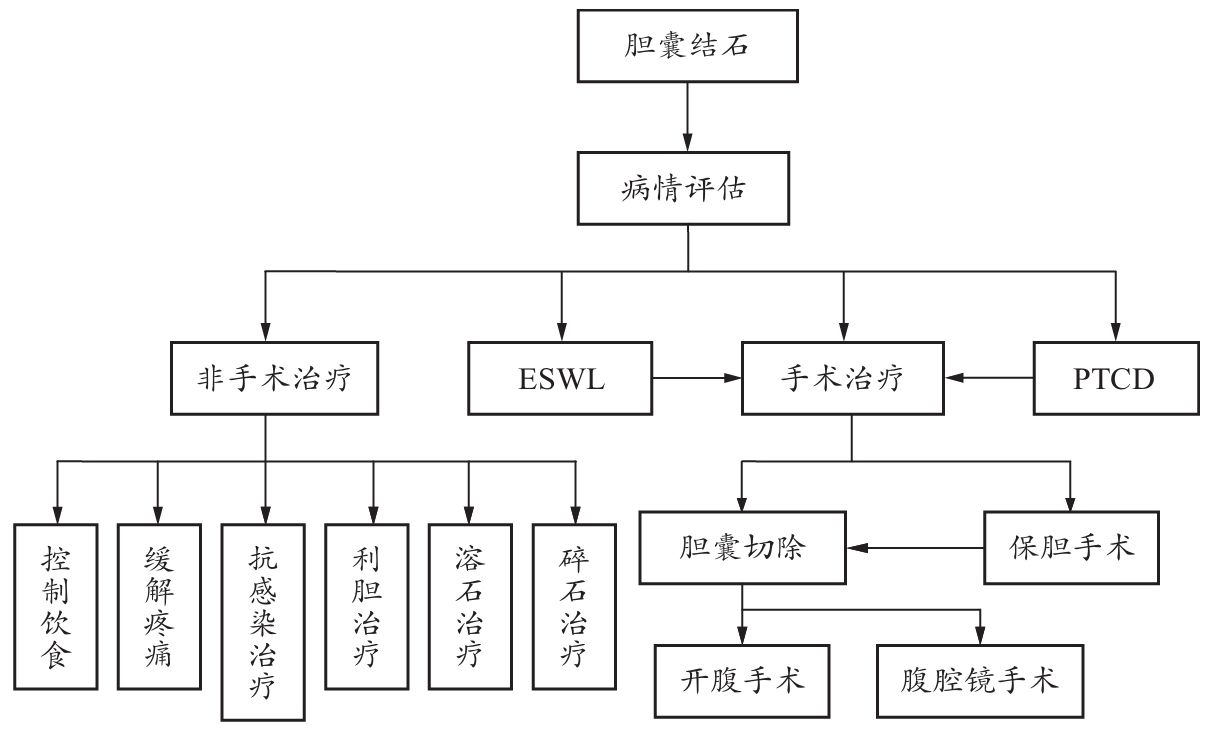
\includegraphics{./images/Image00111.jpg}
 \captionsetup{justification=centering}
 \caption{胆囊结石的治疗程序}
 \label{fig3-20-1}
  \end{figure} 

2. 肝外胆管结石的治疗程序(图\ref{fig3-20-2})

\begin{figure}[!htbp]
 \centering
 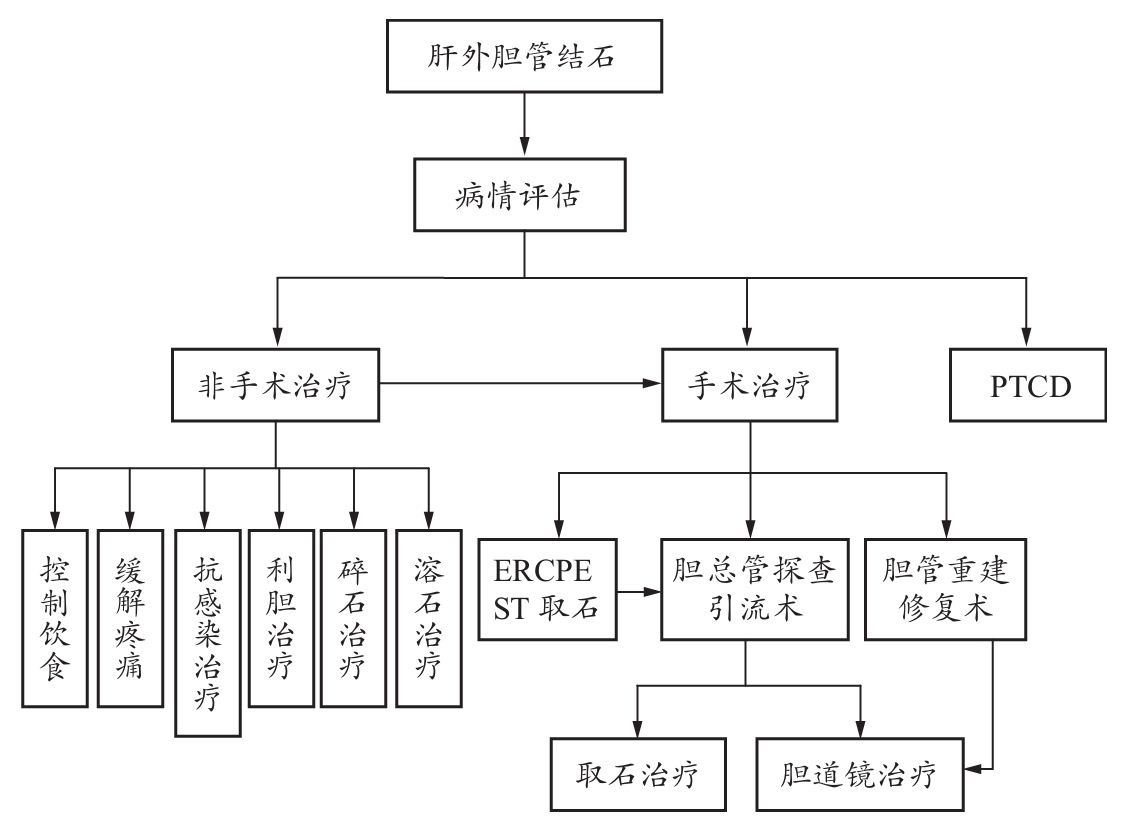
\includegraphics{./images/Image00112.jpg}
 \captionsetup{justification=centering}
 \caption{肝外胆管结石的治疗程序}
 \label{fig3-20-2}
  \end{figure} 

3. 肝内胆管结石的治疗程序 如图\ref{fig3-20-3}所示。

\begin{figure}[!htbp]
 \centering
 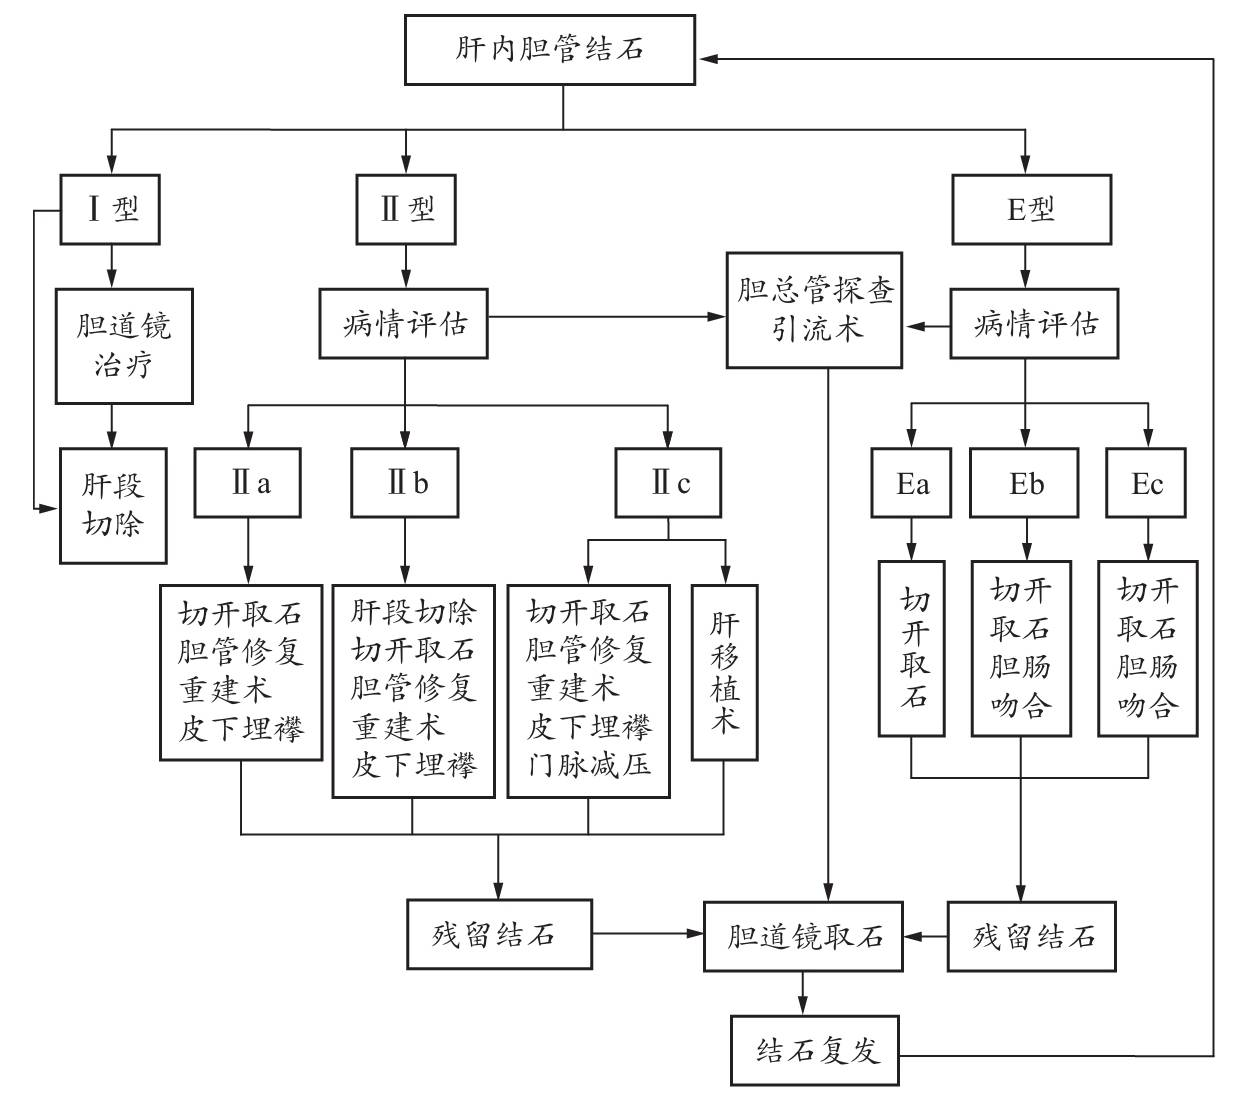
\includegraphics{./images/Image00113.jpg}
 \captionsetup{justification=centering}
 \caption{肝内胆管结石的治疗程序}
 \label{fig3-20-3}
  \end{figure} 

【治疗方案】

1. 非手术疗法

(1)一般治疗:主要包括卧床休息、禁食或低脂饮食、输液、纠正水电解质和酸碱平衡紊乱等。有休克应加强抗休克的治疗,待度过急性期后4\textasciitilde{}6周再行确定性胆道手术,可使患者免受再次手术的痛苦。

(2)解痉镇痛治疗:硝酸甘油、阿托品、哌替啶(度冷丁)或布桂嗪(强痛定)、但吗啡能引起奥迪括约肌痉挛故属禁忌。

(3)抗感染治疗:常选用广谱抗生素,尤对革兰阴性杆菌敏感的抗生素和抗厌氧菌的药物,最好按照细菌培养结果来选择。

(4)利胆治疗:硫酸镁松弛壶腹部括约肌,使滞留的胆汁易于排出。舒胆通、消炎利胆片或清肝利胆口服液等口服,发作缓解后方可应用。

2.
溶石治疗 包括口服溶石药物治疗和局部注射溶石药物治疗。常用口服药物有鹅去氧胆酸和熊去氧胆酸。注射溶石指经皮经肝胆囊置管或经十二指肠镜置入鼻胆导管,将导管与胆石接触,注入溶石剂进行溶石治疗。溶解胆固醇结石的药物有单辛脂、甲基叔丁醚。溶解胆色素结石的药物有二甲基亚砜胺(DM50)、依他酸钠(Na-EDTA)、六甲基磷酸钠(Na-HMP)、苎烯、乙硫基乙酸等。体外实验证实这些药物均有一定的溶石作用,但因接触溶石效果并不理想且有一定的毒副作用而限制了其临床应用。

3.
体外冲击波(震波)碎石术(ESWL) 利用液电、压电或磁电产生冲击波碎石,其疗效取决于结石的性质、大小、数量、钙化程度及其冲击波的能量、碎石次数、胆囊功能等因素,胆石经击碎后可自行排出。同时配合口服溶石药物(CDCA、UDCA)及ERCP网篮取石、乳头肌切开或放置胆道支架效果更好。

4.
内镜治疗 包括内镜下逆行胰胆管造影(ERCP)、内镜下十二指肠乳头切开(EST)及取石、碎石术。必要时可行胆管引流包括支架内引流术及鼻胆管引流术,以解除胆道梗阻,降低胆道压力。适应证如下:胆总管结石,胆总管狭窄,胆囊结石合并胆总管结石,反复发作的胆石性胰腺炎(或伴有胆囊结石)以及其他胆系疾病,包括胆道蛔虫症、急性梗阻性化脓性胆管炎、壶腹部恶性肿瘤性梗阻及奥迪括约肌功能障碍等。

5.
经皮肝穿刺胆道引流术(PTD) 对胆管严重梗阻或化脓性胆管炎者,可行PTD术,以引流胆道、降低胆道压力、控制感染、减少病死率、赢得手术时间等。

6.
胆道镜治疗 包括术中胆道镜、经T管胆道镜、经皮经肝胆道镜等。可取尽胆管结石,并观察胆管粘膜病变,对可疑病变进行病理学检验。对复发结石可通过皮下埋襻用胆道镜取石。

7. 手术治疗

(1)胆囊切除术:包括开腹胆囊切除术及腹腔镜胆囊切除术。

(2)胆囊造瘘术:近年已不常用,仅适用于胆囊周围炎性粘连严重切除胆囊困难很大,可能误伤胆(肝)总管等重要组织者;胆囊周围脓肿,胆囊坏疽、穿孔腹膜炎病情危重者;或年老全身情况衰竭、不能耐受胆囊切除术者。

(3)胆总管探查引流术:是治疗胆管结石的基本方法。目的为探查胆道通畅的情况,取出其中结石,冲洗胆道,T管引流,消除胆道感染。

(4)胆管重建修复术:

1)胆总管十二指肠吻合术:分侧-侧吻合与端-侧吻合两种。手术指征为:缩窄性十二指肠乳头炎胆总管明显增粗,直径在2.0cm以上者;慢性胰腺炎所致的胆总管下端较长范围的管状狭窄与梗阻:原发性胆管结石、慢性胆管炎、复发性胆管结石等。吻合口应\textgreater{}2.0cm,并尽量低位,应切除胆囊。

2)奥迪括约肌切开成形术:本手术实质上是一种低位胆总管十二指肠吻合术,其手术指征、注意事项同胆总管十二指肠吻合术。当胆总管直径在1.5\textasciitilde{}2.0cm以内时,胆总管下端结石嵌顿、其下端狭窄范围不长者,同时合并有胰管开口狭窄者,应选用本手术。

3)胆管空肠Roux-Y吻合术:本手术是治疗胆管结石、胆管炎常用的手术方法。适应证为:慢性化脓性胆管炎、胆(肝)总管明显扩大者;复发性胆管结石胆管明显扩张者;胆道残余结石合并复发性胆管炎者;肝内胆管结石、无法清除干净的结石或肝内广泛结石者。其吻合方式以端-侧、侧-侧和端-侧-侧吻合较为常用。

(5)肝叶(段)切除术:适用于肝内胆管结石多局限于一侧肝叶(段)内不能采用其他手术取净结石者,或肝组织有萎缩者。应切除病变肝叶(段),以根除病灶。

(6)肝移植术:适用于肝脏和胆管系统均已发生弥漫的不可逆性的损害和功能衰竭的Ⅱc型肝胆管结石。

【疗效观察与随访】

1.
观察指标 常见症状与指标、肝功能的代偿情况、全身情况及手术耐受能力。总胆红素、碱性磷酸酶(ALP)、γ-谷氨酰转肽酶(γ-GT)、血清转氨酶(ALT、AST)、乳酸脱氢酶(LDH)、凝血酶原时间测定。B超、CT、MRI、MRCP等无创检查,创伤性检查包括经内镜逆行胆管造影(ERCP)及经皮肝穿刺胆道造影(PTC),必要时可行术中胆道造影。

2. 治愈标准 术后症状、体征消失、无并发症、相关检测指标恢复正常。

3.
随访 注意病情观察,避免并发症,定期复查ALT、AST、α-GT、肝胆B超,必要时复查CT、MRI、PTC等。

【治疗经验与解析】

1.
根据病史、临床表现及检查结果评估肝脏及胆道系统的病变情况、肝功能的代偿情况、全身情况及手术耐受能力,选择适当的手术时机和手术方案。因长时间的胆道感染,屡发胆道梗阻、肝实质损害全身状况较差常有营养不良、消瘦纳差、低蛋白血症、贫血、黄疸等,术前需要改善营养状况,纠正水电解质及酸碱失衡,必要时输血或血浆、人血白蛋白等,并以中西医结合治疗,改善患者全身状况增进食欲,增强手术的耐受力。

2.
ERCP+EST是胆总管结石的首选治疗方法,胆总管结石合并胆囊结石的患者先行ERCP+EST治疗后1周即可行LC切除胆囊结石。胆源性胰腺时首先行ERCP+EST及鼻胆管引流术,以解除胆道梗阻,降低胆胰管压力,减少并发症的发生率及死亡率,但需在72小时内急诊治疗。对于结石过多过大,病情较重无法耐受治疗,可置入支架引流,改善梗阻及胆管炎症状,争取手术时间。

3.
对于肝内胆管结石患者,以往以手术切肝方法为主。随着胆道镜技术的成熟,通过胆总管探查术置入T管,术后2个月经胆道镜取石结合激光碎石可取尽所有结石,改善肝功能。

\subsection{急性胆囊炎}

急性胆囊炎(acute
cholectcystitis)指由于胆囊管梗阻、化学性刺激和细菌感染引起的急性胆囊炎症性病变。临床表现为发热、右上腹疼痛和压痛、恶心、呕吐、轻度黄疸和外周血细胞计数增高等表现。若同时出现寒战、高热、黄疸,应考虑胆管炎。

【治疗方案】

1. 内科治疗

(1)一般治疗:注意休息,禁食、伴有严重呕吐者可放置胃肠引流管,减少胆汁分泌、利于胆汁引流。注意补液、水电解质平衡和营养支持治疗。

(2)解痉镇痛治疗:可使用阿托品、硝酸甘油、哌替啶等药物解除壶腹部括约肌痉挛。

(3)抗感染治疗:选择在血和胆汁中浓度较高的抗生素,必要时根据血和胆汁中细菌培养和药物敏感试验结果更换抗生素。常用的有氨苄西林、克林霉素、氨基糖苷类、三代头孢菌素和喹诺酮类等抗生素。

(4)利胆治疗:硫酸镁松弛壶腹部奥迪括约肌,使滞留的胆汁易于排出。舒胆通、消炎利胆片或清肝利胆口服液等口服,发作缓解后方可应用。

2.
外科治疗 胆囊切除术是急性胆囊炎的根本治疗方法。手术指征:①有急性胆囊炎并发症者;②经内科积极治疗,病情继续发展并恶化者;③急性胆囊炎反复发作者;④无手术禁忌证,能耐受手术者。包括开腹手术和腹腔镜胆囊切除术两种。腹腔镜治疗目前被认为是急性胆囊炎的首选治疗方法。

3.
保胆治疗 如胆囊内有结石残留,可采用微创保胆取石手术用胆道镜在术中彻底取出胆囊内的结石。

【疗效观察与随访】

1.
观察指标 常见症状与体征、血象、血清胆红素、ALT、AST、γ-GT、AKP肝胆B超等。

2.
治愈标准 治疗后症状、体征消失、各相关检测指标恢复正常,肝胆B超正常,无并发症。

3.
随访 注意病情观察,避免并发症,把握手术时机。定期复查AKP、γ-GT、ALT,肝胆B超。

【治疗经验与解析】

1.
当诊断明确且患者一般状况良好时,可在发病的第1日或第2日进行手术;如果合并其他疾病(通常是心肺系统疾病)尚需治疗以减少手术的危险性,胆囊切除术也可延期进行,但要继续进行治疗;若急性胆囊炎缓解,则胆囊切除术可延至6周后进行;如果腹痛进行性加重,并出现白细胞增高和发热,怀疑并发胆囊积脓,坏疽或穿孔时,应紧急进行手术治疗。

2.
急性非胆石性胆囊炎往往发生于创伤、手术、烧伤、败血症或危重病的成人和儿童,是一种严重的疾病。长期胃肠道外营养也可导致胆汁淤积和急性非结石性胆囊炎。临床病程常呈暴发性,保守治疗常伴有坏疽和穿孔。胆囊切除术为最佳治疗方法。不耐受手术者,可给予经皮胆囊造口。

3. 如合并有胆总管结石,可采用ERCP及EST治疗。择期再行腹腔镜胆囊切除术。

4.
胆囊切除术后,一部分患者会出现新的或复发性胆绞痛样疼痛,其发病机制及临床病程尚未完全了解。目前认为,终端胆管及括约肌的壶腹部结构和功能紊乱,引起的乳头狭窄,使胆汁流和(或)胰液分泌受阻,而引起腹痛,极少数患者可能因为以往的炎症或手术损伤,而引起括约肌区的乳头纤维化,或有小的残留结石,逆行性胰胆管造影和括约肌测压可能对诊断是有益的,同时行括约肌切开术是有效的治疗手段。

\subsection{慢性胆囊炎}

慢性胆囊炎(chronic
cholecystitis)是胆囊的慢性炎症性病变,可由结石、慢性感染、化学刺激及急性胆囊炎迁延发作所致,临床上表现为慢性反复发作性上腹部隐痛、消化不良等。当有典型的临床表现,超声检查提示胆囊壁增厚、胆囊萎缩者即可诊断。

【治疗方案】

1.
一般治疗 注意休息,低脂饮食,提高饮食中蛋白质比例。每日蛋白质供给量以每公斤体重1.0\textasciitilde{}1.2g为宜,但要避免随着蛋白质摄入过量的胆固醇。

2. 内科治疗

(1)解痉镇痛治疗:腹痛明显者可使用抗胆碱能药物解除平滑肌痉挛。

(2)溶石治疗:仅适用于胆固醇结石,结石无钙化及胆囊管通畅,胆囊收缩正常者,可服用熊去氧胆酸或鹅去氧胆酸。

(3)利胆治疗:如硫酸镁、消炎利胆片、清肝利胆口服液、保胆健素等。

(4)中药治疗:以清利肝胆、疏肝行气、调理气机、利胆治疗为主。

3.
外科治疗 手术治疗是根治方法,包括手术和腹腔镜下胆囊切除术。反复发作的慢性胆囊炎,伴有胆结石、胆囊积水、胆囊钙化的均可采用外科治疗。

【疗效观察与随访】

1.
观察指标 常见症状与体征、血象、血胆红素、肝功能、AKP、γ-GT、肝胆B超检查等。

2. 治愈标准 症状、体征消失、相关检查指标恢复正常,3个月内无复发。

3.
随访 注意病情观察,避免术后并发症的发生。内科保守治疗无效或加重时采取外科治疗。定期复查AKP、血胆红素、肝功能及胆肺B超等。

【治疗经验与解析】 慢性非胆石性胆囊炎的临床表现由胆囊的病理生理所决定,包括炎症、运动障碍、流出道梗阻、胆囊动力减弱等。反复发作者可行腹腔镜胆囊切除术。

\section{黄疸}

黄疸是高胆红素血症的临床表现,即血中胆红素增加,而使巩膜、皮肤、粘膜以及其他组织和体液发生黄染的现象。正常血中胆红素不过17μmol/L(1.0mg/dl),如胆红素超过正常值而肉眼仍未能察见时,即为隐性或亚临床黄疸。黄疸不是一个独立疾病,而是许多疾病的一种症状和体征,多见于肝脏、胆系和胰腺疾病。黄疸是肝功能不全的一种重要的病理变化,但并非所有的黄疸都是肝功能障碍引起的,例如溶血性黄疸,肝外胆管阻塞引起的阻塞性黄疸,为叙述方便,合并一起讨论。

【治疗程序】 如图\ref{fig3-21-1}所示。

\begin{figure}[!htbp]
 \centering
 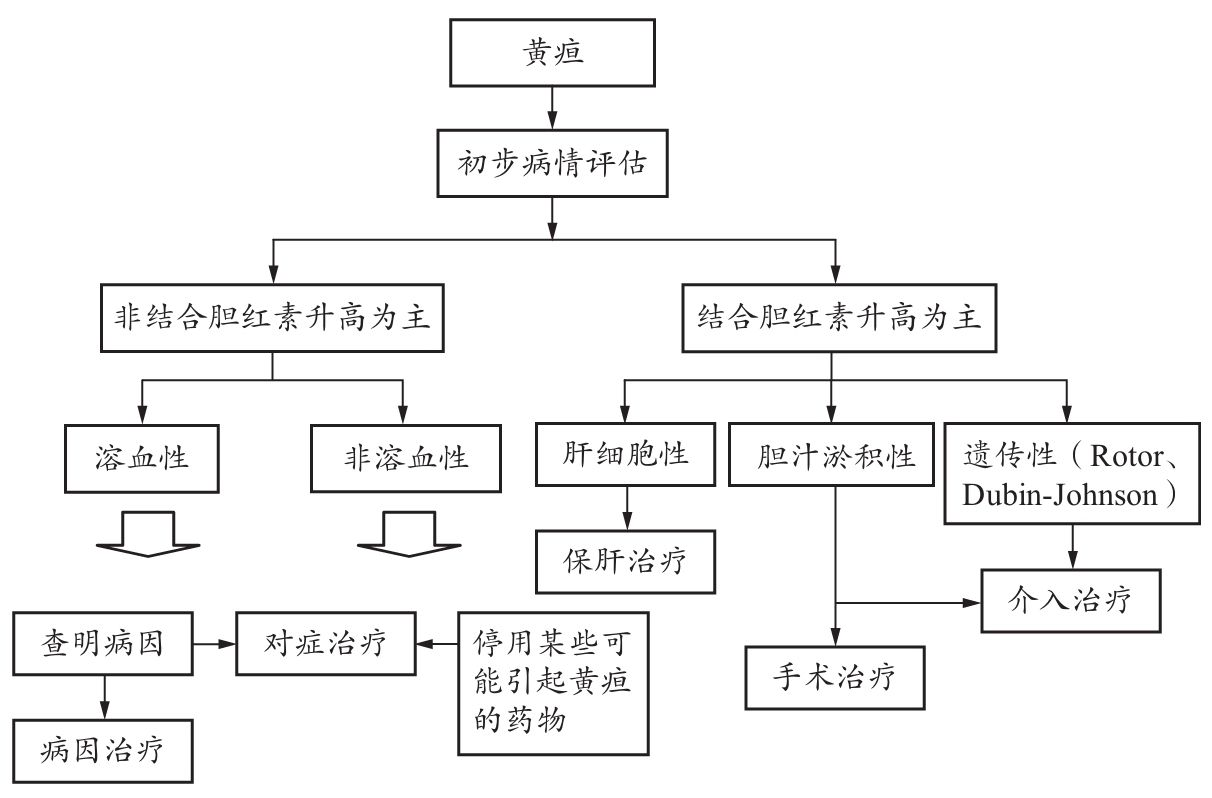
\includegraphics{./images/Image00114.jpg}
 \captionsetup{justification=centering}
 \caption{黄疸的治疗程序}
 \label{fig3-21-1}
  \end{figure} 

【治疗方案】

1.
一般治疗 对症处理,休息,避免肝损因素,如某些特殊药物、酒精、劳累,适当保肝治疗。支持治疗:如调整脂肪供应的类型或数量、中链甘油三酯(40g/d)、补充维生素A、维生素D、维生素E、维生素K和活性钙剂等。

2. 药物治疗

(1)使用消胆胺、苯巴比妥、5-HT{3}
受体拮抗剂、阿片类受体拮抗剂治疗瘙痒症状,其他用药如肾上腺皮质激素、苯巴比妥、熊去氧胆酸、腺苷蛋氨酸(思美泰)、还原性谷胱甘肽等。

(2)介入治疗:内镜下胆管引流术(Endoscopic biliary
drainage,EBD);外引流:经内镜鼻胆管引流(ENBD);内引流:经内镜放置胆道支架(塑料或可膨式金属支架);经皮经肝穿刺胆道引流:可作外引流或(和)内引流,可在阻塞部位置入支架,引流效果同EBD。

(3)病因治疗:是最根本的治疗环节。药物性黄疸停用有关药物;肝外梗阻性黄疸多需手术或经内镜及介入治疗;肿瘤需手术切除或者联合放化疗等综合处理。

【疗效观察与随访】

1. 观察指标

(1)症状、体征:观察瘙痒、腹痛情况、尿、粪颜色,皮肤、巩膜黄染程度,皮肤有无抓痕、出血点,有无肝掌、蜘蛛痣,肝、脾、胆囊是否肿大、有无腹水及进展情况等。病情呈进行性加重抑或波动性或基本稳定。

(2)肝功能检查:

1)血清胆红素测定:血清胆红素分直接胆红素和总胆红素两种。前者相当于结合胆红素(CB),正常不超出3.4μmol/L(0.2mg/dl),总胆红素(TB)系结合和非结合胆红素之和,以非结合胆红素为主,正常不超出17μmol/L(1.0mg/dl)。

2)尿液中胆红素:溶血性黄疸尿液不含胆红素,肝细胞性和梗阻性黄疸均呈阳性反应。

3)尿液中尿胆原:急性大量溶血时,尿液中尿胆原显著增加,慢性少量溶血时,尿胆原含量变化不大。肝细胞性黄疸时,尿液尿胆原可增加;肝内胆淤时则可减少,甚至消失。肝外梗阻时尿中多无尿胆原,尤其是癌性黄疸。

4)粪中尿胆原:梗阻性黄疸时可见下降,结石性梗阻常为不完全性,而癌性梗阻则可完全性。长期粪中尿胆原减少(\textless{}mg/24小时),提示癌性黄疸。

5)蛋白质代谢试验:血清蛋白定量、蛋白电泳分析对黄疸的鉴别意义不大。血浆白蛋白下降见于严重肝实质损害,如慢性肝炎、失代偿期肝硬化和晚期肝癌。血浆球蛋白升高和白蛋白、球蛋白比例倒置见于活动性慢性肝病和结缔组织病等。血浆总蛋白的变化在肝细胞性黄疸时比较明显。长期肝外梗阻和胆汁性肝硬化,血浆α{2}
和β球蛋白明显增高。

6)血胆固醇、胆固醇酯和蛋白X(LP-X)测定:反映肝细胞的脂质代谢功能以及胆系的排泄功能。

7)血清胆汁酸测定:胆汁酸在肝内合成及分泌,正常人血清中含量不超过10μmol/L。肝胆疾病时,胆汁酸代谢发生紊乱。肝细胞对胆汁酸与胆红素摄取和排泄机制不同,在非结合型高胆红素血症如Gilbert症及溶血性黄疸时,并不存在胆汁酸潴留,故有助于黄疸鉴别。

8)血清酶学检查:测定血清酶学对黄疸的病因诊断可有一定帮助。临床上常用的血酶有两大类:①反映肝细胞损害的酶类,主要有丙氨酸氨基移换酶(ALT)及门冬氨酸氨基移换酶(AST),其他还有氨酸琥珀酸裂解酶(ASAL)、醛缩酶(ALD)、精氨酸酶(ARG)和鸟氨酸氨甲基移换酶(ChE)。②反映胆道病变的酶类,如碱性磷酸酶(ALP)和γ-谷氨酰转肽酶(γ-GT)、亮氨酸肽酶(LAP)和5'核苷酸酶(5'{-}NT)等酶,有助于黄疸的鉴别诊断。如一次测定ALT、AST、OCT、ALP、γ-GT和5'NT等6种酶。如前3种酶上升则为肝细胞性黄疸,而后3种增加的则为梗阻性黄疸。但血酶检查无助于鉴别肝内胆瘀和肝外梗阻性黄疸(参阅病毒性肝炎章节)。

9)血浆凝血酶原时间测定:维生素K在肝细胞内能促使凝血酶原形成。肝细胞性黄疸时,凝血酶原的形成减少,凝血酶原时间延长。维生素K系脂溶性,在肠内经胆盐作用始成为水溶性而被吸收,故梗阻性黄疸时凝血酶原时间也可延长。

10)染料排泄功能试验:靛青绿(ICG)排泄试验ICG入血流后,迅速与白蛋白结合而被肝细胞摄取,在肝内经代谢后直接由胆道排入肠道,故能正确反映肝细胞排泄功能。正常人按0.5mg/kg体重的ICG量作静脉注射,15分钟后静脉内滞留量为0\textasciitilde{}10\%。另可参照肝功能Child-Pugh分级标准进行动态评估(见表\ref{tab3-21-1}\footnote{如果是PBC(原发性胆汁性肝硬化)或PSC(原发性硬化性胆管炎):总胆红素(μmol/L):17\textasciitilde{}68为1分,68\textasciitilde{}170为2分,\textgreater{}170为3分;分级:A级:5\textasciitilde{}6分 B级:7\textasciitilde{}9分C级:\textgreater{}10分(包括10分)})。

\begin{table}[htbp]
    \centering
    \caption{Child-Pugh肝功能分级标准}
    \label{tab3-21-1}
    \begin{tabular}{llll}
\toprule
评分指标 & 1分 & 2分 & 3分\tabularnewline
\midrule
肝性脑病(分级) & 无 & 1\textasciitilde{}2 &
3\textasciitilde{}4\tabularnewline
腹水 & 无 & 轻度 & 中、重度\tabularnewline
总胆红素(μmol/L) & \textless{}34 & 34\textasciitilde{}51 &
\textgreater{}51\tabularnewline
白蛋白(g/L) & \textgreater{}35 & 28\textasciitilde{}35 &
\textless{}28\tabularnewline
凝血酶原时间延长(秒) & \textless{}4 & 4\textasciitilde{}6 &
\textgreater{}6\tabularnewline
\bottomrule
    \end{tabular}
\end{table}


2.
治愈标准 黄疸消退,症状消失,引起黄疸的原因解除,各项相关检查指标恢复正常,3个月内未复发。

3.
随访 注意病情观察,症状、体征等变化,避免肝损因素,避免合并症、并发症。必要时定期复查血清胆红素、肝功能、肝胆B超等。

【治疗经验与解析】 明确病因,针对病因是治疗本病最根本的环节。

\section{消化道出血}

\subsection{食管胃底静脉曲张出血}

食管胃底静脉曲张出血(EGVB)是指由于肝硬化等病变引起的门静脉高压,致使食管和(或)胃底静脉曲张,在压力升高或静脉壁发生损伤时,曲张静脉发生破裂出血,临床上主要表现为呕血、黑便、便血和周围循环衰竭征象。EGVB的病因可见于所有引起门静脉高压的疾病,在我国以肝硬化最为常见。

【治疗程序】 如图\ref{fig3-22-1}所示。

\begin{figure}[!htbp]
 \centering
 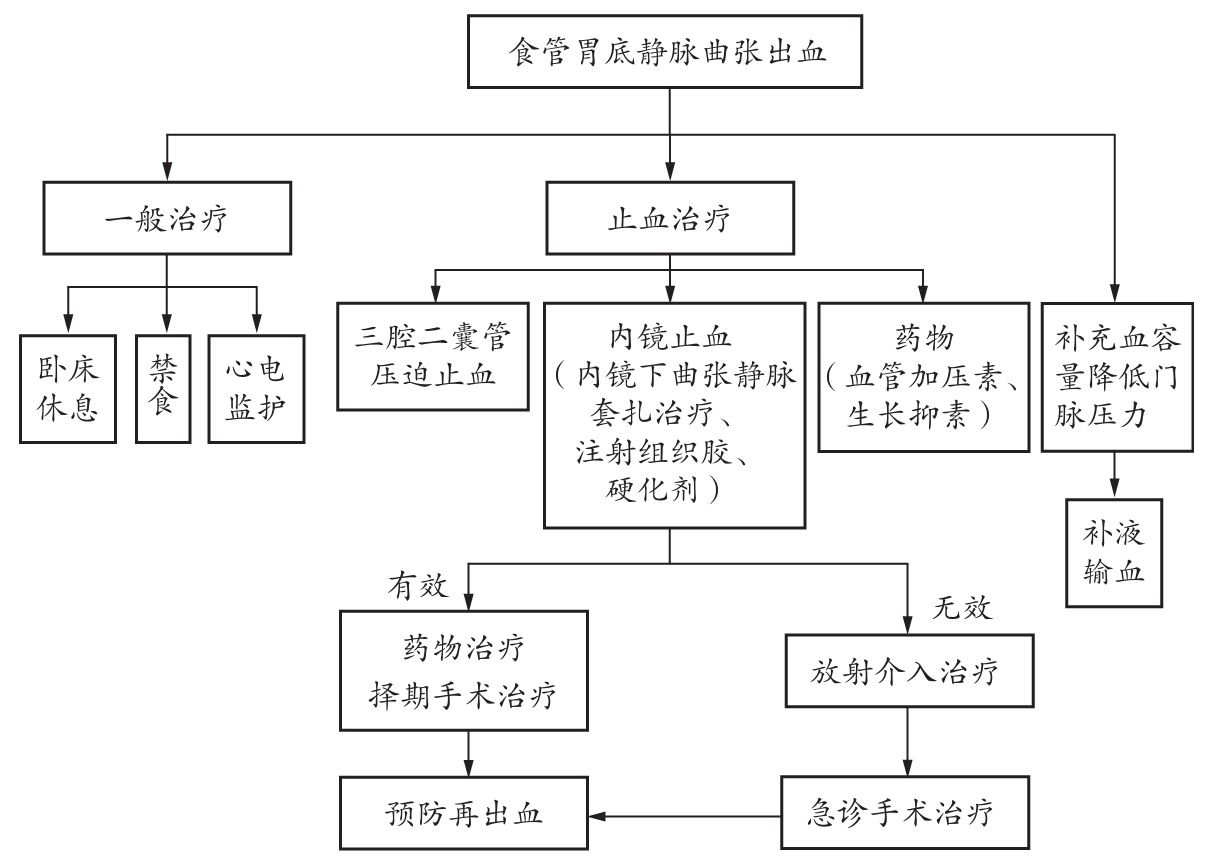
\includegraphics{./images/Image00115.jpg}
 \captionsetup{justification=centering}
 \caption{食管胃底静脉曲张出血的治疗程序}
 \label{fig3-22-1}
  \end{figure} 

【治疗方案】

1. 综合治疗

(1)补充血容量:EGVB出血量一般较大,普遍存在血容量不足,应积极进行液体复苏,恢复有效血容量。对于急性大量出血者,应尽可能施行中心静脉导管置管和中心静脉压监测,以指导液体复苏。短时间内输入大量液体过度扩容后,有诱发再出血和腹水的危险。对高龄、心肺肾疾患者,防止输液量过多,以免引起急性肺水肿。输血指征:①收缩压\textless{}80mmHg,或较基础收缩压降低\textgreater{}30mmHg。②血红蛋白\textless{}50g/L,血细胞压积\textless{}25\%。③心率增快\textgreater{}120次/分。

(2)预防并发症:应积极采取措施保护气道,预防感染,预防肝性脑病,保护肾脏功能,防治水电解质、代谢紊乱等并发症的发生。

2. 止血治疗

(1)药物治疗:目前认为有效的止血药物主要有血管加压素及其类似物和生长抑素及其类似物(如奥曲肽),适用于无法施行内镜治疗或止血失败者,或与内镜治疗联合应用。

1)生长抑素及其类似物:奥曲肽(如善宁)50μg先静脉推注,后以25\textasciitilde{}50μg/h,静脉维持;持续应用3\textasciitilde{}5日;或生长抑素(如思他宁)250μg静推后,以250μg/h,静脉维持3\textasciitilde{}5日,如仍有出血,可增加剂量至500μg/h,静脉维持。

2)血管加压素及其类似物:血管加压素0.4U/kg静脉推注后,以0.4\textasciitilde{}1.0U/(kg·min)持续静滴,联合硝酸甘油10\textasciitilde{}50μg/min,静脉滴注。

(2)内镜治疗:止血方法主要有内镜下曲张静脉硬化治疗(EIS)和内镜下曲张静脉套扎治疗(EVL),是控制活动性出血和预防再出血的主要措施。内镜下注射组织胶也可以有效地止血,但有心、肺和脑血管栓塞等并发症。

(3)气囊填塞:将三腔双囊管或四腔双囊管插入上消化道内,将胃气囊和(或)食管气囊充气以压迫曲张静脉达到止血目的,是一种行之有效的急救方法,其疗效确切,对控制急性出血成功率高。但气囊放气后再出血率高,部分患者有并发食管溃疡和吸入性肺炎的危险。该方法目前仅作为临时性急救措施。

(4)放射介入:放射介入疗法如颈静脉肝内门体分流术(TIPS)可有效地控制出血,但明显增加肝性脑病的危险,适用于对药物和内镜治疗难以控制的曲张静脉出血和等待肝移植的患者。

(5)外科手术:急诊外科手术控制曲张静脉出血和预防再出血的效果确实,但围手术期病死率高,术后肝性脑病发生率高。仅在药物和内镜治疗无效、无法施行TIPS的情况下方可使用。Child-Pugh
C级肝硬化患者不宜施行急诊外科手术。

【疗效观察与随访】

1.
观察指标 观察治疗后意识状态、脉搏和血压、肢体温度、皮肤和甲床色泽、周围静脉特别是颈静脉充盈情况、尿量等,记录呕血、黑便和便血的频度、颜色、性质、次数和总量,定期复查红细胞计数、血红蛋白、Hct与血尿素氮等,查凝血酶原时间、肝功能、肾功能、电解质;必要时留置胃管、导尿管和行气管插管。监测意识障碍和排尿困难者需留置导尿管,危重大出血者必要时进行中心静脉压、血清乳酸测定,老年患者常需心电、血氧饱和度和呼吸监护。

2. 疗效判定

治愈标准:出血停止,血压稳定,病因解除,半年内未复发。

好转标准:出血停止,血压稳定,病因尚未解除,半年内未复发。

3.
随访 ①对于初次内镜检查未发现食管胃静脉曲张者,应3年后复查内镜;对于发现细小曲张静脉者,应每1\textasciitilde{}2年复查内镜;对于酗酒、严重肝功能损害和曲张静脉表面有红色征者,曲张静脉增长速度很快,应每年复查内镜。②除了对患者按时进行随访外,应注重对患者的教育,避免触发、诱发因素的方法。长期使用非选择性β受体阻滞剂,避免骤然停药。有出血倾向时应及时就医。通过长期规范治疗能够有效预防出血,特别是再出血。

【治疗经验与解析】

1.
应立即建立静脉通道,抽血查血型交叉和备血600\textasciitilde{}1200ml,查血常规、凝血酶原时间、肝功能、肾功能、电解质;监测生命体征;必要时留置胃管、导尿管和行气管插管。一般不宜将血红蛋白浓度升至90g/L以上;以免诱发再出血。大量输血时应补充凝血因子、钙等。血小板\textless{}50×10$^{9}$
/L者,可输注血小板;凝血酶原时间延长者应补充凝血酶原复合物。

2.
首次急性静脉曲张出血后,具有较高的再出血率和病死率。2/3的患者可能在2个月内再出血,非选择性β受体阻滞剂可显著降低大静脉曲张患者首次出血的风险,是预防出血唯一理想的成本P效益的药物。由于难以无创简便地测定患者的门静脉压力和肝静脉压力梯度,临床可以根据患者心率是否降低25\%作为剂量有效指标,当心率降至55次/分应考虑停药。

3.
内镜下套扎治疗(EVL)预防静脉曲张再出血的疗效优于硬化剂治疗,平均再出血率约32\%。EVL需每7\textasciitilde{}14日重复治疗1次,直到静脉曲张闭塞,通常需要2\textasciitilde{}4次,以后需3\textasciitilde{}6个月进行胃镜检查以评估静脉曲张有否复发和进行再一次EVL治疗。ELV的并发症发生率大约14\%,通常轻微,常见并发症是短暂的吞咽困难和胸部不适。此外,皮圈套扎部位浅表溃疡也常见,可能会引起出血。可在EVL治疗的患者中使用质子泵抑制剂(如潘托拉唑)。内镜治疗联合药物治疗是最合理的方法,当患者在单用EVL或β受体阻滞剂时发生静脉曲张出血(首次或者再次),力荐ELV和非选择性β受体阻滞剂联合治疗。

4.
门体分流是预防再出血非常有效的方法,但会明显增加肝性脑病发生的风险,且对提高生存率并无影响。TIPS和内镜相比疗效相似,两者在病死率方面没有显著差异。因此TIPS不推荐作为一线治疗方法,而是作为药物联合内镜治疗无效时的一种补救措施。

\subsection{急性非静脉曲张性上消化道出血}

急性非静脉曲张性上消化道出血(ANVUGIB)指屈氏韧带以上的消化道的非静脉曲张性疾患引起的出血,包括胰管或肝管的出血和胃空肠吻合术后吻合口附近疾患引起的出血。

【治疗程序】 如图\ref{fig3-22-2}所示。

\begin{figure}[!htbp]
 \centering
 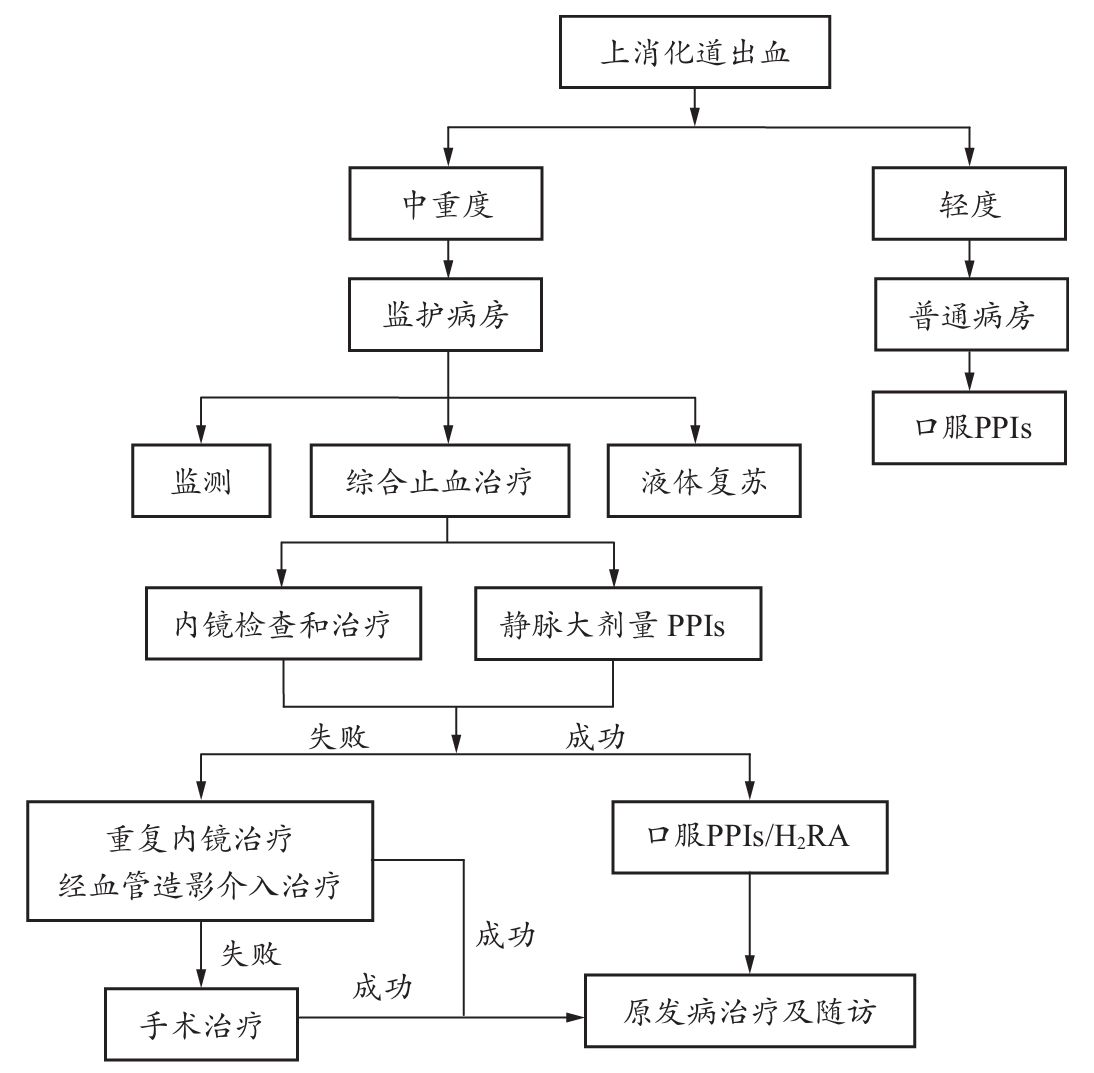
\includegraphics{./images/Image00116.jpg}
 \captionsetup{justification=centering}
 \caption{急性非静脉曲张性上消化道出血的治疗程序}
 \label{fig3-22-2}
  \end{figure} 

【治疗方案】

1.
出血征象监测 ①记录呕血、黑便和便血的频率、颜色、性质、次数和总量,定期复查红细胞计数、血红蛋白、Hct与血尿素氮等。对活动性出血或重度ANVUGIB患者应插入胃管,以观察出血停止与否。②监测意识状态、脉搏和血压(注意排除服用受体阻滞剂和抗胆碱能药物对脉搏和血压的影响)、肢体温度、皮肤和甲床色泽、周围静脉特别是颈静脉充盈情况、尿量等。意识障碍和排尿困难者需留置导尿管,危重大出血者必要时进行中心静脉压测定,老年患者常需心电、血氧饱和度、呼吸监护。③判断失血量:病情严重度与失血量呈正相关,常根据临床综合指标判断失血量的多寡。临床可以根据血容量减少导致周围循环的改变(伴随症状、脉搏和血压、化验检查)来判断失血量(表\ref{tab3-22-1})。

\begin{table}[htbp]
\centering
\caption{上消化道出血病情严重程度分级}
\label{tab3-22-1}
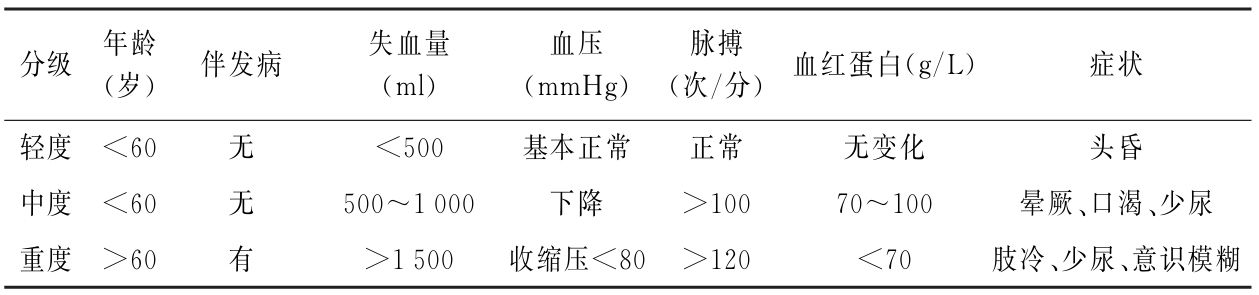
\includegraphics{./images/Image00117.jpg}
\end{table}

2. 液体复苏

(1)建立静脉通道:应立即建立快速静脉通道,并选择较粗静脉以备输血,最好能留置导管。根据失血的多少在短时间内输入足量液体,以纠正血循环量的不足。对高龄、伴心肺肾疾病患者,应防止输液量过多,以免引起急性肺水肿。对于急性大量出血者,应尽可能施行中心静脉压监测,以指导液体的输入量。当意识恢复;四肢末端由湿冷、青紫转为温暖、红润,肛温与皮温差减小(1℃);脉搏由快弱转为正常有力,收缩压接近正常,脉压差大于30mmHg;尿量多于30ml/h;中心静脉压恢复正常时,提示血容量已补足。

(2)液体的种类和输液量:常用液体包括等渗葡萄糖液、生理盐水、平衡液、血浆、全血或其他血浆代用品。紧急时输液、输血同时进行。输血指征为:①收缩压\textless{}90mmHg,或较基础收缩压降低幅度\textgreater{}30mmHg。②血红蛋白\textless{}50\textasciitilde{}70g/L,Hct\textless{}25\%。③心率增快(\textgreater{}120次/分)。

(3)血管活性药物:在补足液体的前提下,如血压仍不稳定,可以适当地选用血管活性药物(如多巴胺)以改善重要脏器的血液灌注。

3. 止血措施

(1)抑酸药物:能提高胃内pH值,既可促进血小板聚集和纤维蛋白凝块的形成,避免血凝块过早溶解,有利于止血和预防再出血,又可治疗消化性溃疡。临床常用的制酸剂主要包括:

1)质子泵抑制剂(PPI):常用的PPI制剂有奥美拉唑、潘妥拉唑、兰索拉唑、雷贝拉唑等。诊断明确后推荐使用大剂量PPI治疗,如埃索美拉唑80mg静脉推注后,以8mg/h输注持续72小时。常规剂量:如埃索美拉唑80mg静脉滴注,12小时1次。

2)组胺H{2} 受体拮抗剂(H{2}
RA):常用药物包括西米替丁、雷尼替丁、法莫替丁等,口服或静脉滴注,可用于低危患者。

(2)内镜下止血:起效迅速、疗效确切,应作为首选。常用止血方法有局部药物喷洒和注射、热凝止血(高频电、氩气血浆凝固术、热探头、微波、激光等)和金属止血夹机械止血等。

(3)止血药物:止血药物对ANVUGIB的确切效果未能证实,不作为一线药物使用,对有凝血功能障碍者,可静脉注射维生素K{1}
;为防止继发性纤溶,可使用止血芳酸等抗纤溶药;云南白药等中药也有一定疗效。

(4)选择性血管造影及栓塞治疗:明确出血部位及病因,必要时栓塞治疗。(5)手术治疗:内镜及介入治疗无效,病情危急者可考虑手术治疗。

【疗效观察与随访】

1. 观察指标

(1)实验室检查:常用化验项目包括胃液或呕吐物或粪便隐血试验、外周血红细胞计数、血红蛋白浓度、红细胞压积等。为明确病因、判断病情和指导治疗,尚需进行凝血功能试验(如出凝血时间、凝血酶原时间)、血肌酐和尿素氮、肝功能、肿瘤标志物等检查。

(2)活动性出血的判断:判断出血有无停止,对决定治疗措施极有帮助。如果患者症状好转、脉搏及血压稳定、尿量足(\textgreater{}30ml/小时),提示出血停止。临床上有以下情况时提示有活动性出血:①呕血或黑便次数增多,呕吐物呈鲜红色或排出暗红血便,或伴有肠鸣音活跃。②经快速输液输血,周围循环衰竭的表现未见明显改善,或虽暂时好转而又恶化,中心静脉压仍有波动,稍稳定又再下降。③红细胞计数、血红蛋白测定与Hct继续下降,网织红细胞计数持续增高。④补液与尿量足够的情况下,血尿素氮持续或再次增高。⑤胃管抽出物有较多新鲜血。

(3)内镜检查:发现溃疡出血,根据溃疡基底特征,可用来判断病变是否稳定,凡基底有血凝块、血管显露等易于再出血,内镜检查时对出血灶病变应作Forrest分级(表\ref{tab3-22-2})。对分级为Ⅰa\textasciitilde{}Ⅱb的应进行内镜下止血。

\begin{table}[htbp]
    \centering
    \caption{出血性消化性溃疡的Forrest分级}
    \label{tab3-22-2}
    \begin{tabular}{lll}
\toprule
Forrest分级 & 溃疡病变 & 再出血概率(\%)\tabularnewline
\midrule
Ⅰa & 喷射样出血 & 55\tabularnewline
Ⅰb & 活动性渗血 & 55\tabularnewline
Ⅱa & 血管显露 & 43\tabularnewline
Ⅱb & 附着血凝块 & 22\tabularnewline
Ⅱc & 黑色基底 & 10\tabularnewline
Ⅲ & 基底洁净 & 5\tabularnewline
\bottomrule
    \end{tabular}
\end{table}

(4)预后的评估:

1)病情严重程度分级:一般根据年龄、有无伴发病、失血量等指标将ANVUGIB分为轻、中、重度。年龄超过65岁、伴发重要器官疾患、休克、血红蛋白浓度低、需要输血者再出血危险性增高。无肝肾疾病患者的血尿素氮或肌酐或血清转氨酶升高者,病死率增高。

2)Rockall评分系统分级:该系统中,积分≥5者为高危,3\textasciitilde{}4分为中危,0\textasciitilde{}2分为低危(表\ref{tab3-22-3})。

\begin{table}[htbp]
\begin{center}
\caption{急性上消化道出血患者的Rockall再出血和死亡危险性评分系统变量}
\label{tab3-22-3}
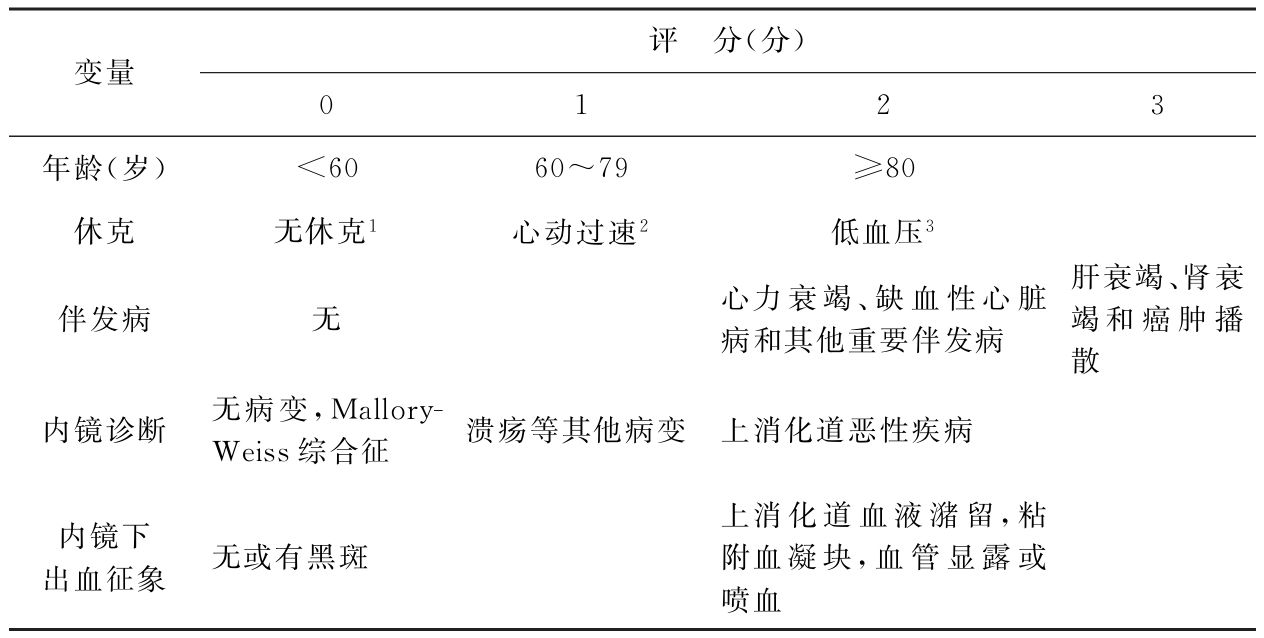
\includegraphics{./images/Image00118.jpg}
\end{center}

注:1:收缩压\textgreater{}100mmHg,心率\textless{}100次/分。

2:收缩压\textgreater{}100mmHg,心率\textgreater{}100次/分。

3:收缩压\textless{}100mmHg,心率\textgreater{}100次/分。

2. 疗效评价 显效:出血停止,相关检测指标恢复正常,原发病缓解。

3.随访 注意病情观察,避免再次出血。定期复查相关指标(见前)。
\end{table}



【治疗经验与解析】

1.
约80\%的消化道溃疡患者出血会自行停止,再出血或持续出血的患者病死率较高,应根据病情进行个体化分级救治,高危患者应多学科协作救治。

2.
内镜是诊断病因的关键,急诊内镜检查,应尽早在24\textasciitilde{}48小时内进行。无法行内镜检查和治疗的先纠正循环衰竭再行检查。检查时进行动脉血氧和心电监护。出血治疗的同时进行原发病的治疗,如消化道溃疡患者Hp阳性者行抗Hp治疗。长期服用NASID药物的患者同时服用PPI或粘膜保护剂。

3. 继续加强对原发病的诊治。

\subsection{下消化道出血}

下消化道出血是指十二指肠空肠移行部、Treiz韧带以下的小肠、结肠和直肠疾病所引起的肠道出血。多数下消化道出血有明显血便,结合临床及必要实验室检查,通过结肠镜全结肠检查,必要时配合X线小肠钡剂造影检查,确诊一般并不困难。

【治疗程序】 如图\ref{fig3-22-3}所示。

\begin{figure}[!htbp]
 \centering
 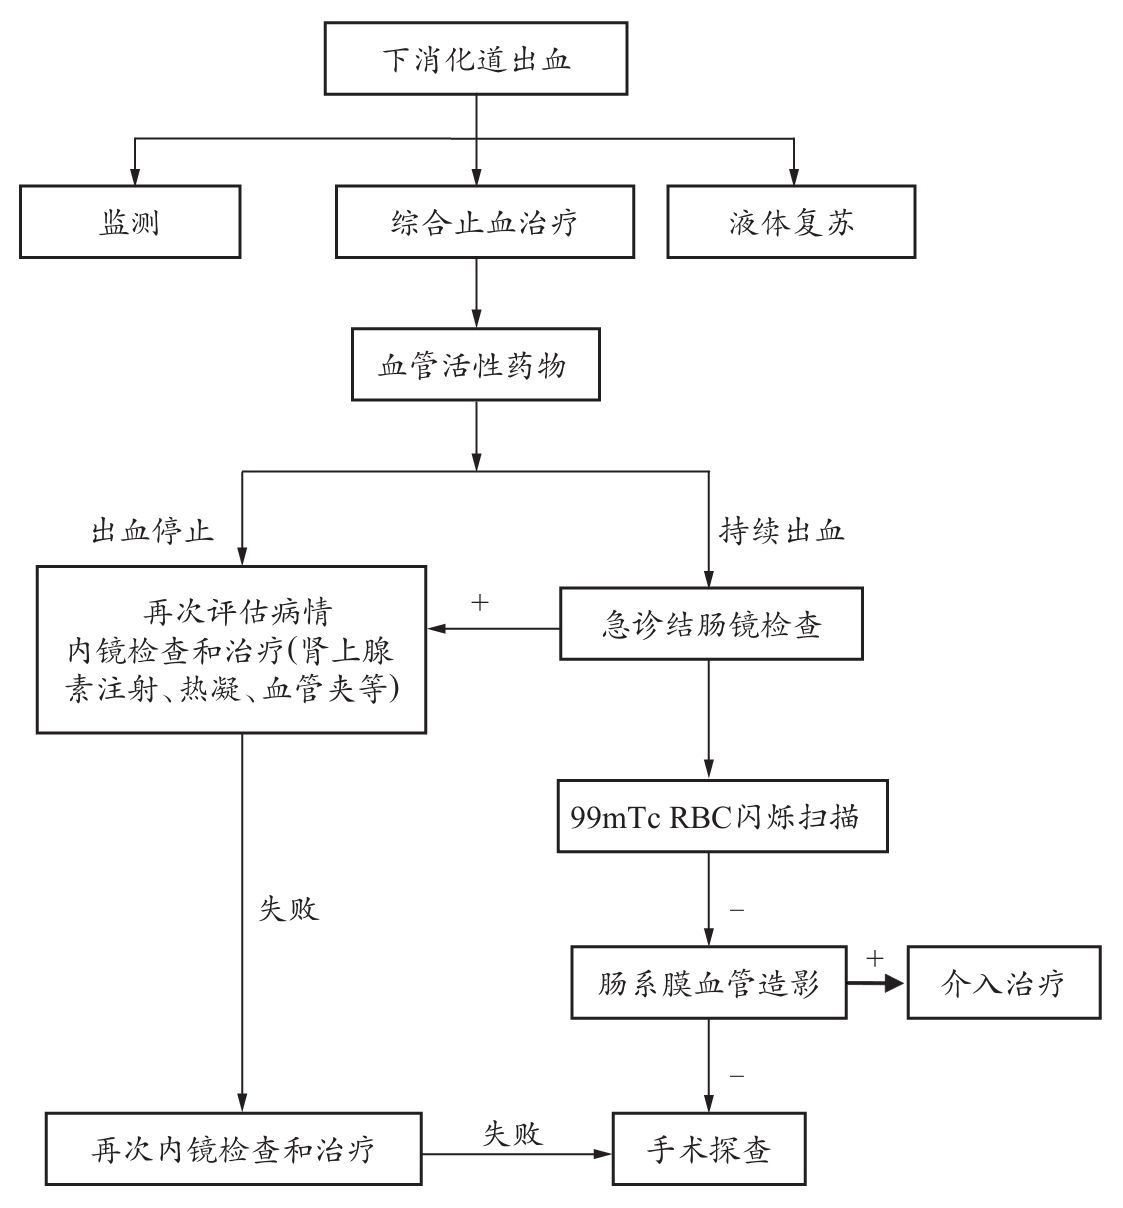
\includegraphics{./images/Image00119.jpg}
 \captionsetup{justification=centering}
 \caption{下消化道出血的治疗程序}
 \label{fig3-22-3}
  \end{figure} 

【治疗方案】

“出血征象监测”和“液体复苏”详见本章相关内容。止血措施如下:

(1)止血药物:血管加压素、生长抑素静脉滴注可有一定作用。

(2)内镜下止血:急诊结肠检查可发现出血病灶,可同时行内镜下止血。常用止血方法有局部药物喷洒和注射、热凝止血(高频电、氩气血浆凝固术、热探头、微波、激光等)和金属止血夹机械止血等。

(3)肠系膜血管造影及血管介入治疗:血管介入止血治疗方法包括血管内药物注射治疗和选择性血管栓塞治疗。改良的超选择性动脉灌注利用加压素直接作用肠系膜动脉或其分支,甚至是末梢血管,起到止血作用。血管介入治疗的优点是简便、安全、创伤小、效果迅速可靠,特别对于消化道大出血患者可起到挽救患者生命的作用。介入治疗止血能够帮助患者渡过难关,为外科手术止血创造条件,成为治疗下消化道出血的有效手段。

(4)手术治疗:内镜及介入治疗无效,病情危急者可考虑手术治疗。

【疗效观察与随访】 参见本章相关内容。

【治疗经验与解析】

1.
下消化道出血病因复杂,诊治方法也较多。内镜治疗、血管介入等治疗方法为诊断治疗的主要方法。外科手术治疗是抢救治疗下消化道大出血的有效手段。多排扫描CT的出现和胶囊内镜、双气囊小肠镜的应用发展,使肠道出血病变的诊治手段更丰富,准确性更高,部位更准确。双气囊小肠镜可进行镜下治疗,弥补了以往小肠内镜检查治疗的不足。内镜和血管介入诊治方法仍将是下消化道出血治疗的主要发展方向。

2.
低位小肠或者右半结肠出血量少,速度慢,在肠道停留时间久,可能为黑便,易误诊为上消化道出血。若上消化道出血量1000ml以上,速度快,大便可呈鲜红色,易误认为下消化道出血。